\documentclass[a4paper,12pt,twoside,spanish]{book}

\usepackage[spanish, es-tabla]{babel}
\usepackage[utf8]{inputenc}
\usepackage{amsfonts}
\usepackage{amssymb}
\usepackage{amsmath}
\linespread{1.25}
\usepackage{time}
\usepackage{rotating}
\usepackage{epsfig}
\usepackage{pifont}
\usepackage{verbatim}
\usepackage{pstricks}
\usepackage{multirow}
\usepackage{units}    
\usepackage{threeparttable}
\usepackage{mathrsfs}    
\usepackage[colorlinks,allcolors=blue]{hyperref}
\usepackage{fancyhdr}
\usepackage{cite}
\usepackage{array}
\usepackage{graphicx}
\graphicspath{ {images/} }
\usepackage{graphics}
\usepackage{gensymb}
\usepackage{subcaption}
\usepackage{caption}
\usepackage{changepage}

\usepackage{herab}

\pagestyle{fancy}
%----------------
\textheight22.6cm \textwidth16.0cm
%\textheight23.0cm \textwidth16.0cm
\newlength{\dinwidth}
\newlength{\dinmargin}
\newlength{\medwwidth}
\setlength{\dinwidth}{21.0cm}
\setlength{\headwidth}{\textwidth}
\setlength{\headheight}{18.0pt}
\columnsep1cm


\setlength{\dinmargin}{\dinwidth}
\addtolength{\dinmargin}{-\textwidth}
\setlength{\dinmargin}{0.5\dinmargin}
\oddsidemargin -1.0in
\setlength{\medwwidth}{-0.4cm}
\addtolength{\oddsidemargin}{\dinmargin}
\addtolength{\medwwidth}{\textwidth}
\setlength{\evensidemargin}{\oddsidemargin}
\setlength{\marginparwidth}{0.9\dinmargin}
\marginparsep 8pt \marginparpush 5pt
\topmargin0.0cm

%----------------------------------
\fancyhead{}
%\fancyhead[LE,RO]{\thepage}
%\fancyhead[LE]{\slshape {\bf \thepage}~~~~ \leftmark}
%\fancyhead[RO]{\slshape \rightmark ~~~~{\bf \thepage}}
\fancyhead[LE,RO]{\thepage}
\fancyhead[RE]{\slshape \leftmark }
\fancyhead[LO]{\slshape \rightmark}
\cfoot{}
%----------------------------------


%===================================
\renewcommand{\chaptermark}[1]{%
  \markboth{%   
    \thechapter~%
      \ #1}
  {}}
\renewcommand{\sectionmark}[1]{%
  \markright{%
    \thesection~%
      \ #1}
  {}}   
\renewcommand{\headrulewidth}{0.6pt}
%===================================






 

\usepackage[bottom=3cm,left=3cm,right=3cm,top=3cm]{geometry}

\usepackage{mathtools}
\DeclarePairedDelimiter\bra{\langle}{\rvert}
\DeclarePairedDelimiter\ket{\lvert}{\rangle}
\DeclarePairedDelimiterX\braket[2]{\langle}{\rangle}{#1 \delimsize\vert #2}

\usepackage{lmodern}
\usepackage[T1]{fontenc}

\usepackage{tikz} 
\usetikzlibrary{shapes,arrows,positioning,automata,backgrounds,calc,er,patterns}
\usepackage{tikz-feynman}
\tikzfeynmanset{compat=1.0.0}

% \renewcommand{\baselinestretch}{1.4}
\newcolumntype{P}[1]{>{\centering\arraybackslash}p{#1}}

%changed!
\newcommand{\Bee}{\ensuremath{{b}}}
\newcommand{\bjpsiX}{\ensuremath{ \Bee\to\jpsi X}}
\newcommand{\bjpsi}{\ensuremath{\Bee \to\jpsi}}
\newcommand{\bjpsill}{\ensuremath{\Bee \to\jpsi\to l^+l^-}}
\newcommand{\bjpsiee}{\ensuremath{\Bee \to\jpsi\to e^+e^-}}
\newcommand{\bjpsimm}{\ensuremath{\Bee \to\jpsi\to \mu^+\mu^-}}
\newcommand{\sigbbar}{\ensuremath{\sigma(\bbar)}}
\newcommand{\dsigbbar}{\ensuremath{\Delta\sigma(\bbar)}}
\newcommand{\bbar}{\ensuremath{\Bee\overline{\Bee}}}
\newcommand{\ccbar}{\ensuremath{c \overline{c}}}
\newcommand{\ttbar}{\ensuremath{t \overline{t}}}

\newcommand{\pntobbar}{\ensuremath{pN\to \bbar }}
%

%\newcommand{\ee}{\ensuremath{{\mathrm e}^+{\mathrm e}^-}}
\newcommand{\ee}{\ensuremath{e^+e^-}}
\newcommand{\mm}{\ensuremath{\mu^+\mu^-}}
\newcommand{\bn}{\ensuremath{{\mathrm B}^0}}
%\newcommand{\Bee}{\ensuremath{{\mathrm b}}}
\newcommand{\bnbar}{\ensuremath{\mathrm \overline{B}^0}}
\newcommand{\bnd}{\ensuremath{\mathrm B^0_d}}
\newcommand{\bndbar}{\ensuremath{\mathrm \overline{B}^0_d}}
\newcommand{\bns}{\ensuremath{\mathrm B^0_s}}
\newcommand{\bnsbar}{\ensuremath{\mathrm \overline{B}^0_s}}
\newcommand{\asym}{\ensuremath{frac{\Gamma_{B^0}(t)   - \Gamma_{\overline{B^0}}(t) }
                         {\Gamma_{B^0}(t)   + \Gamma_{\overline{B^0}}(t) } } }
\newcommand{\jpsi}{\ensuremath{J/\psi}}
\newcommand{\jpsiX}{\ensuremath{\mathrm \jpsi X}}
%\newcommand{\bjpsiX}{\ensuremath{\mathrm b\to\jpsi X}}
%\newcommand{\bjpsi}{\ensuremath{\mathrm b\to\jpsi}}
\newcommand{\jpsill}{\ensuremath{\mathrm \jpsi\to l^+l^-}}
\newcommand{\jpsiee}{\ensuremath{\mathrm \jpsi\to e^+e^-}}
\newcommand{\jpsimm}{\ensuremath{\mathrm \jpsi\to \mu^+\mu^-}}
%\newcommand{\bjpsill}{\ensuremath{\mathrm b\to\jpsi\to l^+l^-}}
%\newcommand{\bjpsiee}{\ensuremath{\mathrm b\to\jpsi\to e^+e^-}}
%\newcommand{\bjpsimm}{\ensuremath{\mathrm b\to\jpsi\to \mu^+\mu^-}}
\newcommand{\ks}{\ensuremath{{\mathrm  K}^{\mathrm 0}_{\mathrm s}}}
\newcommand{\K}{\ensuremath{{\mathrm  K}^+}}
%\newcommand{\bbar}{\ensuremath{\mathrm \B\overline{\Bee}}}
%\newcommand{\sigbbar}{\ensuremath{\sigma(\bbar)}}
\newcommand{\xf}{\ensuremath{x_{ F}}}
\newcommand{\pt}{\ensuremath{p_{ T}}}


\newcommand{\dm}{\ensuremath{\Delta m} }
\newcommand{\dmd}{\ensuremath{\Delta m_{\mathrm d}}}
\newcommand{\egev}{\ensuremath{\, \mathrm{GeV}}}
\newcommand{\mgev}{\ensuremath{\, \mathrm{GeV}/c^2}}
\newcommand{\pgev}{\ensuremath{\, \mathrm{GeV}/c}}
\newcommand{\emev}{\ensuremath{\, \mathrm{MeV}}}
\newcommand{\etev}{\ensuremath{\, \mathrm{TeV}}}
\newcommand{\mmev}{\ensuremath{\, \mathrm{MeV}/c^2}}
\newcommand{\pmev}{\ensuremath{\, \mathrm{MeV}/c}}
\newcommand{\mum}{\ensuremath{\, \mu\mathrm m}}
\newcommand{\acp}{\ensuremath{a_{\mathrm CP}}}
\newcommand{\ccp}{\ensuremath{c_{\mathrm CP}}}
\newcommand{\ecp}{\ensuremath{\epsilon_{\mathrm B}} }

\newcommand{\tosolve}[1]{{\color{red}  *** #1}}

\newcommand{\met}{\ensuremath{E_{T}^{\text{miss}}}} 
                      


%%%%%%%%%%%%%%%%%%%%%%%%%%%%%%%%%%%%%%%%%%%%%%%%%%%%%%%%%%%%%%%%
\begin{document}



\pagenumbering{gobble}


\newgeometry{top=2cm,bottom=1.5cm,left=3cm,right=3cm}


\thispagestyle{empty}
\begin{center}

\begin{figure}[h]
\centering

\includegraphics[width=0.4\textwidth]{escudo.pdf}
\end{figure}

{\normalsize Universidad Nacional de La Plata\\}
{\normalsize Facultad de Ciencias Exactas\\}
{\normalsize Departamento de Física\\}

% \hline

\vspace{2cm}

\hrulefill

{\bf \LARGE  Estudios de fondos de electrones reconstruidos como fotones en búsquedas de Supersimetría con el detector ATLAS\\}

\vspace{0.6cm}

\hrulefill

\vspace{0.3cm}

{\normalsize \bf Trabajo de Diploma \\}

\vspace{2.5cm}

{\Large \bf Gonzalo E. Orellana \\}

\vspace{3.5cm}

{\large\bf Director \\}
{\large\bf Dr. Hernán P. Wahlberg \\}

\vspace{2cm}

{\normalsize Marzo 2017}

\end{center}



\restoregeometry



 

\thispagestyle{empty} 
\cleardoublepage

\pagenumbering{roman}    

\tableofcontents  
   
\cleardoublepage 

\pagenumbering{arabic}

\setcounter{page}{1}

\pagestyle{fancy}

\chapter{Modelo Estándar y Supersimetría}
% \addcontentsline{toc}{chapter}{Modelo Estándar y Supersimetría}
\chaptermark{Modelo Estándar y Supersimetría}


El Modelo Estándar (SM, por sus siglas en inglés) es la teoría que describe a las partículas elementales y a sus interacciones. Este modelo fue introducido por Glashow, Salam y Weinberg en la década de los 70 \cite{Glashow:1961tr,Salam:1968rm,Weinberg:1967tq}. Está basado en teorías cuánticas de campo, y sus predicciones, cuantitativas y cualitativas, han sido verificadas experimentalmente con gran precisión.

Una de las extensiones del SM mejor motivada desde el punto de vista teórico es la Supersimetría, ya que resuelve algunas de las limitaciones del mismo. En particular, provee una solución al problema de jerarquía, proporciona candidatos para la materia oscura, permite la unificación de las fuerzas del SM, y hasta propone una conexión entre estas y la gravedad. Es por este motivo, que la Supersimetría, se ha vuelto uno de los objetivos principales en la búsqueda de nueva física en los últimos años.

\section{Modelo Estándar}
 
Según el SM las partículas se clasifican en dos grandes grupos: fermiones y bosones. Los fermiones son los que componen la materia ordinaria y se caracterizan por obedecer la estadística de Fermi-Dirac y tener espín semientero. Estos se clasifican en leptones y quarks, según si experimentan o no la interacción fuerte, siendo los últimos los que pueden interactuar mediante dicha fuerza.  

Existen 6 tipos (o sabores) de leptones que se clasifican en tres generaciones. Cada generación se forma a partir de un leptón masivo y cargado y otro no masivo y neutro. Así se tienen el electrón ($e^{-}$) con su correspondiente neutrino ($\nu_{e}$), y el muón ($\mu^{-}$) y el tau ($\tau^{-}$) con sus neutrinos asociados ($\nu_{\mu}$ y $\nu_{\tau}$ ).


Así mismo, existen 6 tipos de quarks: up ($u$), down ($d$), charm ($c$), strange ($s$), top ($t$) y bottom ($b$). A diferencia de los leptones, lo quarks tienen carga de color, que les permite interactuar mediante la fuerza fuerte. Los quarks solo se manifiestan en estados ligados, denominados hadrones, fenómeno conocido
como confinamiento de quarks. Existen dos tipos de hadrones en la naturaleza: los bariones ($qqq$) y los mesones ($q\bar{q}$).

Los fermiones se pueden encontrar en dos estados de helicidad, izquierda y derecha, salvo los neutrinos que solamente existen en estados de helicidad izquierda. Las dos últimas generaciones de fermiones son inestables, por lo que decaen a las de la primera generación. Es por esto que la materia ordinaria está compuesta por fermiones de la primera generación.

Así como los fermiones están asociados a la materia, los bosones están asociados a los portadores de las interacciones. Los mismos se caracterizan por obedecer la estadística Bose-Einstein y por tener espín entero. Existen cuatro tipos de interacciones fundamentales. La electromagnética, que afecta a las partículas con carga eléctrica, cuyo bosón asociado es el fotón. La débil, que actúa tanto en los quarks como en los leptones, asociada a los bosones $W^{\pm}$ y $Z^{0}$. La interacción fuerte, que actúa en las partículas con carga de color, cuyo portador son los gluones. Finalmente, la cuarta interacción es la gravitatoria. La misma no está descripta por el SM, pero supone que debería actuar sobre todas las partículas del SM y su bosón asociado sería el gravitón.

Todas las partículas anteriormente mencionadas, tienen asociadas una antipartícula con la misma masa y espín, pero con carga y varios de sus números cuánticos opuestos (isospín, charmness, strangeness, topness, número bariónico, etc.). 

El SM se construye formalmente como una teoría de gauge no abeliana, imponiendo invarianza de gauge local sobre campos cuantificados que describen las partículas fundamentales, dando lugar a los campos de gauge que describen las interacciones. Su grupo de simetría es:

\begin{equation}
\mathcal{G}_{SM}=SU(3)_{C}\times SU(2)_{L}\times U(1)_{Y}
\end{equation}

\noindent
donde $Y$ (la hipercarga), $L$ (la helicidad izquierda) y $C$ (la carga de color) representan las cantidades conservadas del grupo de simetría. El subgrupo $SU(2)_{L}\times U(1)_{Y}$ representa el sector electrodébil (QED + interacción débil) y el subgrupo $SU(3)_{C}$ incluye la cromodinámica cuántica (QCD).


En el SM las partículas adquieren su masa mediante el mecanismo de Brout-Englert-Higgs (BEH) \cite{Englert:1964et,Higgs:1964ia,Higgs:1964pj,Guralnik:1964eu,Higgs:1966ev,Kibble:1967sv} , a partir de la ruptura espontanea de la simetría electrodébil:

\begin{equation}
\mathcal{G}_{SM}\rightarrow SU(3)_{C}\times U(1)_{Q}
\end{equation}

\noindent
produciendo los bosones masivos $W^{\pm}$ y $Z^{0}$. Como consecuencia, es necesario incluir en el lagrangiano un nuevo campo escalar, dando lugar a un nuevo bosón masivo de espín 0, llamado bosón de Higgs. El mismo fue descubierto en el año 2012 por las colaboraciones ATLAS y CMS \cite{Aad:2012tfa, Chatrchyan:2012xdj}. La medida más reciente de su masa se determinó con un valor de $125.09 \pm 0.21 (\text{estad.}) \pm 0.11 (\text{sist.}) \egev$ \cite{Aad:2015zhl}. Así como los bosones de gauge adquieren su masa mediante este mecanismo, es posible también generar la masa de los fermiones mediante su interacción con el Higgs, completando de esta forma el espectro de masas del SM. La Tabla \ref{smparticles} expone algunas propiedades de las partículas mencionadas.

\renewcommand{\arraystretch}{1.3}
\begin{table}	
\centering
\caption{Partículas elementales del SM.}
\begin{tabular}{ l | c  c  c | c c }

	\hline

		& \multicolumn{3}{c}{Partículas} & Espín & Carga eléctrica \\

	\hline

	\multirow{3}{*}{Quarks} & $(u,d)_{L}$ & $(c,s)_{L}$ & $(t,b)_{L}$ & $(\frac{1}{2},\frac{1}{2})$ & $(\frac{2}{3},-\frac{1}{3})$ \\

							& $u_{R}$ & $c_{R}$ & $t_{R}$ & $\frac{1}{2}$ & $\frac{2}{3}$ \\

							& $d_{R}$ & $s_{R}$ & $b_{R}$ & $\frac{1}{2}$ & $-\frac{1}{3}$ \\

	\hline

	\multirow{2}{*}{Leptones} 	& $(\nu_{e},e^{-})_{L}$ & $(\nu_{\mu},\mu^{-})_{L}$ & $(\nu_{\tau},\tau^{-})_{L}$ & $(\frac{1}{2},\frac{1}{2})$ & $(0,-1)$ \\

								& $e_{R}^{-}$ & $\mu_{R}^{-}$ & $\tau_{R}^{-}$ & $\frac{1}{2}$ & $-1$ \\

	\hline

	\multirow{2}{*}{Bosones de Gauge} 	& \multicolumn{3}{c |}{$g$} & $1$ & $0$ \\

										& \multicolumn{3}{c |}{$W^{\pm}$, $Z$} & $1$ & $\pm1, 0$ \\

	\hline

	Bosones escalares & \multicolumn{3}{c |}{$H$} & 0 & 0 \\

	\hline

\end{tabular}
\label{smparticles}
\end{table}
\renewcommand{\arraystretch}{1}

Como comentario final, el SM tiene 19 parámetros libres: las 9 masas de los fermiones (considerando que los neutrinos tienen masa nula), las 3 constantes de acoplamiento de las interacciones, los 3 ángulos de mezcla de la matriz Cabibbo-Kobayashi-Maskawa (CKM) junto con la fase de la violación CP, el ángulo de vacío de QCD y finalmente la masa del Higgs y su valor de expectación del vacío.


\subsection{Física más allá del Modelo Estándar}

El SM provee una descripción notablemente exitosa de todos los fenómenos accesibles con los experimentos de altas energías disponibles actualmente. Sin embargo, también se sabe que el SM deja cuestiones sin resolver, tanto desde el punto de vista teórico, como experimental.

Desde el punto de vista teórico, el SM no explica los números cuánticos como la carga eléctrica, el isospín, la hipercarga o el color. Tampoco explica por qué los fermiones izquierdos se agrupan en dobletes y los derechos en singletes, ni por qué hay tres cargas de color, o cuántas generaciones hay. Otro síntoma de incompletitud es la gran cantidad de parámetros libres (19) que deben ajustarse a los datos observados, ya que no resultan de principios teóricos más fundamentales.

Desde el punto de vista experimental, también existen algunos resultados que no pueden acomodarse dentro del SM. Distintos experimentos demostraron que si bien los neutrinos tienen una masa muy pequeña, la misma no es nula. En contraposición con el SM que considera a los mismos no masivos. De todas formas, es posible escribir un término de masa para los neutrinos en el lagrangiano \cite{Drewes:2013gca}. El mismo requiere agregar parámetros adicionales a la teoría y además, de la existencia de neutrinos con quiralidad derecha, que aún no fueron observados.

El SM tampoco provee un candidato para la materia oscura. A partir de la observación del movimiento de las galaxias, se sabe que el mismo no se corresponde con la cantidad de materia observada, y es por eso que se propone la existencia de materia indetectable para los instrumentos astronómicos de medición actuales. La materia oscura debería corresponder entonces a partículas masivas, que interactúen solo débilmente y gravitacionalmente.

El triunfo de la teoría electrodébil, parece indicar que todas las interacciones corresponden a distintas manifestaciones de un único campo unificado y que el SM es una teoría efectiva a bajas energías (del orden de los $100\egev$). Incluso ante la ausencia de la gran unificación de las fuerzas electrodébil y fuerte a una escala muy alta de energía, el SM debería ser modificado para incorporar los efectos de la gravedad a la escala de Planck $M_{P} \simeq 10^{19} \egev$. En este contexto, es un misterio por qué la relación $M_{W}/M_{P} \simeq 10^{-17} \egev$ es tan pequeña, lo que se denomina <<problema de jerarquía>>\cite{PhysRevD.14.1667}. Esto lleva a pensar que los fenómenos de nueva física existen 17 órdenes de magnitud por arriba de la energía explorada en el presente. Asociado a este problema está el llamado <<problema de naturalidad>>, donde no se comprende por qué la masa del Higgs es tan pequeña comparada con masa de Planck.


\subsection{Divergencias cuadráticas}

Como se mencionó anteriormente, el SM ha tenido un gran éxito en la descripción de los fenómenos conocidos hasta la escala del TeV. Aun así, es clara la necesidad de construir una nueva teoría que solucione los problemas que el SM conlleva. El principal inconveniente es solucionar el <<problema de jerarquía>>, en el cual el cociente de escalas $M_{W}/M_{P}$ es muy pequeño. Para ello es necesario ver las consecuencias de esta diferencia de escalas.

La parte eléctricamente neutra del campo de Higgs del SM es un escalar complejo $H$ con un potencial clásico $V=m_{H}^{2}|H|^{2}+\lambda|H|^{4}$. El SM necesita un valor de expectación de vacío (VEV) para $H$ no nulo, en el mínimo del potencial. Esto ocurre si $\lambda >0$ y $m_{H}^{2}<0$, resultando en $\left\langle H \right\rangle = \sqrt{-m_{H}^{2}/2\lambda}$. Experimentalmente, de las medidas de las propiedades de las interacciones débiles, se sabe que el valor de $\left\langle H \right\rangle$ es de aproximadamente 174 GeV. El descubrimiento del bosón de Higgs en el 2012 con una masa cercana a 125 GeV implica que, suponiendo que el SM es correcto como una teoría efectiva, $\lambda = 0.126$ y $m_{H}^{2}=-(92.9\: \egev)^{2}$.

Por cada partícula a la que se acopla el campo de Higgs, $m_{H}^{2}$ recibe una gran corrección cuántica de los efectos virtuales. Por ejemplo, si el campo de Higgs se acopla a un fermión $f$ con un término en el lagrangiano igual a $-\lambda H\bar{f}f$, el diagrama de Feynman en la Figura \ref{loops} genera una corrección:

\begin{equation}
\Delta m_{H}^{2}=-\frac{|\lambda_{f}|^{2}}{8\pi^{2}}\Lambda_{UV}^{2}+...
\label{fermion_corr}
\end{equation}

\noindent
donde $m_{f}$ es la masa del fermión y $\Lambda_{UV}$ es el corte usado para regular la integral en el loop. 

\begin{figure}
\centering

	\begin{subfigure}{0.45\textwidth}
	\begin{tikzpicture}
	\begin{feynman}
	\vertex (a) {\(H\)};
	\vertex [right=2cm of a] (b);
	\vertex [above right=of b] (e);
	\vertex [below right=of b] (f);
	\vertex [above right=of f] (c);
	\vertex [right=2cm of c] (d);
	\diagram* {
	(a)-- [scalar] (b),
	(b)-- [fermion, quarter left, edge label=\(f\)] (e),
	(e)-- [quarter left] (c),
	(c)-- [quarter left, fermion] (f),
	(f)-- [quarter left] (b),
	(c)-- [scalar] (d),
	};
	\end{feynman}
	\end{tikzpicture}
	\end{subfigure}
	\hfill
	\begin{subfigure}{0.45\textwidth}
	\begin{tikzpicture}
	\begin{feynman}
	\vertex (a) {\(H\)};
	\vertex [right=3cm of a] (b);
	\vertex [above left=of b] (d);
	\vertex [above right=of b] (f);
	\vertex [above right=of d] (e);
	\vertex [right=3cm of b] (c);
	\diagram* {
	(a)-- [scalar] (b),
	(b)-- [scalar, quarter left] (d),
	(d)-- [quarter left, scalar, edge label=\(S\)] (e),
	(e)-- [quarter left, scalar] (f),
	(f)-- [quarter left, scalar] (b),
	(b)-- [scalar] (c),
	};
	\end{feynman}
	\end{tikzpicture}
	\end{subfigure}

\caption{Correcciones cuánticas a un \textit{loop} al parámetro de masa del Higgs $m_{H}^{2}$ debido a la masa de un fermión de Dirac \textit{f} (izquierda) y debido a la masa de un campo escalar \textit{S} (derecha).}
\label{loops}
\end{figure}

Si $\Lambda_{UV}$ es del orden de $M_{P}$, la corrección a $m_{H}^{2}$ es 30 órdenes de magnitud más grande que el valor requerido $\sim (100\: \egev)^{2}$, produciendo las divergencias cuadráticas. Si bien los fermiones y bosones de gauge no tienen este comportamiento cuadrático en las correcciones cuánticas (sus masas son “naturales”), también se ven afectados indirectamente por este efecto, ya que las masas de los mismos dependen de $\left\langle H \right\rangle$. De esta forma, todas las masas de SM se ven afectadas por la escala de corte $\Lambda_{UV}$.

Una forma de solucionar este problema consiste en considerar la existencia de un escalar complejo $S$ de masa $m_{S}$, que se acopla al campo de Higgs con un término $-\lambda_{S} |H|^{2}|S|^{2}$. El diagrama de Feynman de la Figura \ref{loops} genera una corrección:

\begin{equation}
\Delta m_{H}^{2}=\frac{\lambda_{S}^{2}}{16\pi^{2}}\left[\Lambda_{UV}^{2}-2m_{S}^{2}\ln(\Lambda_{UV}^{2}/m_{S})+... \:\right]
\label{boson_corr}
\end{equation}

% \begin{figure}
% \centering
% \begin{tikzpicture}
% \begin{feynman}
% \vertex (a) {\(H\)};
% \vertex [right=3cm of a] (b);
% \vertex [above left=of b] (d);
% \vertex [above right=of b] (f);
% \vertex [above right=of d] (e);
% \vertex [right=3cm of b] (c);
% \diagram* {
% (a)-- [scalar] (b),
% (b)-- [scalar, quarter left] (d),
% (d)-- [quarter left, scalar, edge label=\(S\)] (e),
% (e)-- [quarter left, scalar] (f),
% (f)-- [quarter left, scalar] (b),
% (b)-- [scalar] (c),
% };
% \end{feynman}
% \end{tikzpicture}
% \caption{Correcciones cuánticas a un \textit{loop} al parámetro de masa del Higgs $m_{H}^{2}$ debido a la masa de un campo escalar \textit{S}.}
% \label{loop_f}
% \end{figure}

De esta forma, si existieran fermiones (bosones) no predichos por el SM, relacionados con los bosones (fermiones) del SM mediante una simetría, las contribuciones a las masas de las Ecuaciones \ref{fermion_corr} y \ref{boson_corr} se cancelarían. A esta simetría se la denomina supersimetría (SUSY, por sus siglas en inglés) \cite{Martin:1997ns}.


\section{Extensión Supersimétrica del Modelo Estándar}

Supersimetría es una simetría que relaciona las masas y los acoplamientos de partículas con diferente espín. Una transformación supersimétrica convierte un estado bosónico en uno fermiónico, y viceversa. El operador $Q$ que genera estas transformaciones debe ser un espinor anticonmutativo, que cumpla:

\begin{equation}
\centering
Q \ket{\text{\,bosón\,}} = \ket{\text{\,fermión\,}}
\qquad\qquad\qquad
Q \ket{\text{\,fermión\,}} = \ket{\text{\,bosón\,}}
\end{equation}

Los espinores son intrínsecamente objetos complejos, por lo tanto el conjugado hermítico de $Q$ es también un generador de la simetría. Debido a que $Q$ y $Q^{\dagger}$ son operadores fermiónicos, llevan momento angular de espín $\frac{1}{2}$, por lo tanto es claro que SUSY debe ser una simetría espacio-temporal.

Los estados de partícula de una teoría supersimétrica son representados en el álgebra de SUSY como supermultipletes. Cada supermultiplete contiene ambos estados, fermión y bosón, que son comúnmente llamados supercompañeros uno de otro. Los generadores $Q$ y $Q^{\dagger}$ conmutan con los generadores de las transformaciones de gauge, por lo tanto las partículas en un mismo supermultiplete tienen que estar en la misma representación del grupo de gauge, y tener la misma carga eléctrica, isospín y color. Y como el operador de masa $-P^{2}$ también conmuta con los generadores y con todos los operadores de rotación y traslación, deberán tener los mismos autovalores de $-P^{2}$ , y entonces la misma masa.

Cada supermultiplete tiene que contener igual número de grados de libertad fermiónico que bosónico ($n_{F}=n_{B}$), por lo que existen varias combinaciones posibles. Las dos más importantes para esta teoría son el supermultiplete quiral (o escalar) y el de gauge (o vectorial).

% El supermultiplete escalar tiene un único fermión de Weyl ($n_{F}=2$) y dos escalares reales ($n_{B}=1$). Estos dos escalares se suelen poner como un único campo escalar complejo.

% El supermultplete vectorial contiene un bosón vectorial de spin $1$. Para que la teoría sea renormalizable, tiene que ser un bosón de gauge no masivo, al menos antes de que la simetría de gauge sea espontáneamente rota. En este caso, este bosón contiene dos estados de helicidad ($n_{B}=2$). Por lo tanto su supercompañero es un fermión de Weyl de espín $\frac{1}{2}$, con dos estados de helicidad ($n_{F}=2$). Si en vez de esto, se intenta usar un fermión de espín $\frac{3}{2}$ la teoría no sería renormalizable. Los bosones de gauge deben transformar como la representación adjunta del grupo de gauge, por lo que sus compañeros fermiónicos, llamados <<gauginos>>, también.En el caso de incluir la gravedad, el gravitón de espín 2 (con dos estados de helicidad, n B = 2) tiene un supercompañero de espín llamado <<gravitino>>.

La inclusión de la Supersimetría resuelve varios de los problemas antes mencionados. La simetría cancela las divergencias cuadráticas en la corrección de la masa del Higgs. La corrección de términos de mayor orden requieren que la masa de la partícula supersimétrica más liviana (\textit{Lightest Supersymmetric Particle}, LSP) sea del orden del TeV, siendo ese el orden de energía en el cual el SM deja de ser válido, y es necesaria la implementación de SUSY. También provee un candidato a materia oscura, siendo en la mayoría de los modelos la partícula supersimétrica más liviana, que es estable y no interactuante. Finalmente, SUSY provee un marco de referencia para una teoría de Gran Unificación y para teorías que incorporan a la gravedad. 



\subsection{Modelo Estándar Supersimétrico Mínimo}

Como se mencionó antes, en una extensión supersimétrica del SM, cada una de las partículas elementales conocidas está contenida en un supermultiplete quiral o de gauge, y debe tener un supercompañero con espín que difiera en $\frac{1}{2}$. La extensión que requiere la introducción de la mínima cantidad de parámetros se conoce como <<Modelo Estándar Supersimétrico Mínimo>> (MSSM por sus siglas en inglés).

Veamos ahora como se van construyendo los distintos supermultipletes. Como los supermultipletes escalares son los únicos que pueden contener un fermión cuya parte izquierda y derecha transforman de forma diferente, todos los fermiones del SM están agrupados en este tipo de supermultiplete. En cuanto a su nomenclatura, los nombres de los compañeros de espín 0 de los quarks o leptones son construidos anteponiendo una “s” (de scalar ), y son llamados <<squarks>> y <<sleptones>>. La parte izquierda y derecha de los quarks y leptones son fermiones de Weyl con diferentes propiedades de transformación de gauge del SM, entonces cada uno debe tener un compañero escalar complejo. Por ejemplo, los supercompañeros de la parte izquierda y derecha del campo de Dirac de los electrones son llamadas $\tilde{e}_{L}$ y $\tilde{e}_{R}$ , aunque el subíndice no se refiere a la helicidad de los slectrones (ya que ambos tienen espín 0) sino a la de sus supercompañeros. Lo mismo aplica para las demás leptones y quarks, los neutrino son simplemente denominados $\tilde{\nu}$ ya que son siempre izquierdos.

El bosón escalar de Higgs debe estar en un supermultiplete quiral ya que tiene espín 0. Dada la naturaleza de los campos quirales introducidos en la implementación de SUSY, el campo escalar de Higgs no es suficiente para dar masa a los fermiones de helicidad izquierda y derecha, por lo que se debe agregar un nuevo campo escalar para compensar. En el SM, el campo de Higgs es un doblete, y de los cuatro grados de libertad solo uno permanece como consecuencia de la ruptura de la simetría electrodébil, resultando en un bosón de Higgs. En el MSSM se necesitan dos dobletes de Higgs, $H_{u}=(H^{+}_{u},H^{0}_{u})$ y $H_{d}=(H^{0}_{d},H^{-}_{d})$. El escalar neutro que corresponde al bosón de Higgs del SM es una combinación lineal de $H^{0}_{u}$ y $H^{0}_{d}$. La nomenclatura usual para referirse a los supercompañeros de espín  es agregar “-ino” a la partícula del SM, por lo tanto los compañeros fermiónicos de los escalares de Higgs son denominados <<higgsinos>>, y se denotan $\widetilde{H_{u}}$ y $\widetilde{H_{d}}$.

Los bosones vectoriales del SM tienen que estar en supermultipletes de gauge y sus supercompañeros fermiónicos son llamados <<gauginos>>. Las interacciones de gauge de color de QCD son mediadas por el gluon, cuyo compañero supersimétrico de espín  es el <<gluino>>. Los gauginos supercompañeros de los bosones de gauge electrodébiles, luego de mezclarse con los supercompañeros de los bosones de Higgs, dan lugar a los autoestados de masa denominados <<charginos>> y <<neutralinos>>. En la Tabla \ref{susyparticles} se puede ver el espectro completo del MSSM.


\renewcommand{\arraystretch}{1.3}
\begin{table}	
\centering
\begin{threeparttable}
\caption{Supermultipletes quirales y de \textit{gauge} del MSSM.}
\begin{tabular}{ P{4cm} P{4cm} P{4cm} }

	\hline

	Supermultiplete & Bosón & Fermión \\

	\hline

	gluón, gluino & $g$ & $\widetilde{g}$ \\

	\hline

	W, wino & $W^{\pm}$, $W^{0}$ & $\widetilde{W}^{\pm}$, $\widetilde{W}^{0}$ \\
	B, bino & B & $\widetilde{B}$ \\

	\hline

	\multirow{2}{*}{sleptón, leptón $^{*}$} 	& $(\widetilde{\nu},\widetilde{e})_{L}$ & $(\nu,e)_{L}$ \\

										& $e_{R}$ & $e_{R}$ \\

	\hline

	\multirow{3}{*}{squark, quark $^{*}$}		& $(\widetilde{u}_{L},\widetilde{d}_{L})$ & $(u_{L},d_{L})$ \\

										& $\widetilde{u}_{R}$ & $u_{R}$ \\

										& $\widetilde{d}_{R}$ & $d_{R}$ \\

	\hline

	\multirow{2}{*}{Higgs, higgsinos}	& $(H^{0}_{d},H^{-}_{d})$ & $(\widetilde{H}^{0}_{d},\widetilde{H}^{-}_{d})$ \\

										& $(H^{+}_{u},H^{0}_{u})$ & $(\widetilde{H}^{+}_{u},\widetilde{H}^{0}_{u})$ \\

	\hline
\end{tabular}
\begin{tablenotes}
\item [*] \footnotesize Junto con las otras dos generaciones.
\end{tablenotes}
\label{susyparticles}
\end{threeparttable}
\end{table}
\renewcommand{\arraystretch}{1}


Por construcción, cada partículas y su supercompañero debe tener la misma masa, por lo que deberían existir, por ejemplo, fotinos de masa nula y selectrones con $0.511 \emev$. Como ninguna de las partículas antes mencionada fue observada experimentalmente, se deduce que SUSY es una simetría que está rota en el estado de vacío elegido por la naturaleza.

El hecho de que sea una simetría rota, impide que se cancelen las divergencias cuadráticas en el cuadrado de las masas escalares, y eso fue uno de los motivos por el cual se introdujo SUSY. Para poder garantizar que siga ocurriendo esa cancelación, la ruptura de la simetría debe ser suave, y el lagrangiano efectivo del MSSM tiene que escribirse como:

\begin{equation}
\mathcal{L}=\mathcal{L}_{\text{SUSY}}+\mathcal{L}_{\text{soft}}
\end{equation}

\noindent
donde $\mathcal{L}_{\text{SUSY}}$ contiene todas las interacciones de gauge y de Yukawa, y preserva la invarianza supersimétrica. 
% El conjunto de parámetros que aparecen en el lagrangiano $\mathcal{L}_{SUSY}$ son:

% \begin{itemize}

% 	\item las constantes de acoplamiento de gauge $g_{s}$, $g$ y $g'$ correspondientes a los grupos de gauge $SU(3)_{C}$, $SU(2)_{L}$ y $U(1)_{Y}$, respectivamente

% 	\item los acoplamientos de Yukawa que describen las interacciones entre fermiones y bosones de Higgs

% 	\item el parámetro de masa del campo de Higgs $\mu$.

% \end{itemize}


El lagrangiano que rompe SUSY, $\mathcal{L}_{\text{soft}}$, no está completamente determinado y su forma explícita así como el conjunto de parámetros involucrados dependen del mecanismo particular de ruptura de SUSY. Debido a que este mecanismo es desconocido, se puede suponer un conjunto de términos de ruptura de la forma más general posible, sin indagar en sus orígenes, que se fijan solo pidiendo la invarianza frente $SU(3)_{C}\times SU(2)_{L}\times U(1)_{Y}$, y que sean suaves a fin de mantener la cancelación de las divergencias cuadráticas. Estos términos soft proveen exitosamente las masas de las partículas supersimétricas, a fin de que sean más pesadas que sus correspondientes compañeras del SM, y la ruptura espontánea de la simetría electrodébil requerida a bajas energías necesaria para explicar la generación de las masas de las partículas del SM. Aun así, la diferencia de masa entre supercompañeros no debe ser demasiado grande, ya que se perdería la solución al problema de jerarquía.

% El conjunto de nuevos parámetros que aparece en el superpotencial de ruptura de SUSY incluye \cite{Agashe:2014kda,Haber:1993wf}:

% \begin{itemize}
 
% 	\item Las masas soft del sector de Higgs, $m_{1}$ , $m_{2}$ y $m_{12}$ , donde $m_{12}^{2} \equiv B\mu$, $\mu$ es el parámetro introducido anteriormente y $B$ es el parámetro de ruptura de SUSY.

% 	\item Las masas soft de los squarks y sleptones de cada generación: $m_{\tilde{Q}}$ , $m_{\tilde{U}}$ , $m_{\tilde{D}}$ , $m_{\tilde{L}}$ y $m_{\tilde{E}}$ .

% 	\item Los acoplamientos trilineales de squarks y sleptones $A_{q}$ y $A_{l}$.

% 	\item Las masas soft de los gauginos, $M_{3}$ , $M_{2}$ y $M_{1}$ , asociadas a los grupos de gauge del $SU(3)_{C}$, $SU(2)_{L}$ y $U(1)_{Y}$, respectivamente.

% \end{itemize}

Adicionalmente, para evitar problemas con la conservación del número bariónico $B$ y leptónico $L$, se introduce una nueva simetría denominada paridad-R. Se define como $P_{R}=(-1)^{3(B-L)+2s}$, donde $s$ es el espín de la partícula. Las partículas supersimétricas tienen $P_{R}=-1$, mientras que las partículas del SM tienen $P_{R}=+1$. La conservación de la paridad-R genera que las partículas supersimétricas solo puedan ser producidas en número par en experimentos de colisiones.

El trabajo de la referencia \cite{Dimopoulos:1995ju} muestra que el MSSM posee 124 parámetros independientes. De estos, 18 corresponden a los parámetros del SM, uno corresponde al sector de Higgs (el análogo a la masa del Higgs del SM), y 105 son nuevos parámetros del modelo. 

Existen distintas propuestas para los mecanismos de ruptura de supersimetría. En la búsqueda asociada al presente trabajo, el modelado de la señal de SUSY se da en el contexto del modelo “Generalised Model of Gauge-Mediated Supersymmetry Breaking” (GGMSB). En este modelo, la supersimetría es rota en la escala del TeV en un sector oculto de estados inaccesibles por procesos del SM, y es propagada al sector visible del MSSM vía interacciones de bosones de gauge del grupo $SU(3)_{C} \times SU(2)_{L} \times U(1)_{Y}$ y gauginos.

En estos modelos con mediaciones de gauge, el gravitino es la partícula supersimétrica más ligera (LSP), con masas del orden del keV, estable y no interactuante, produciendo así energía faltante en la reconstrucción del evento en su estado final.

\subsection{El espectro de masas}

Los supercompañeros de las partículas del SM no son necesariamente los estados de masa del MSSM. Incluyendo efectos de ruptura de simetría electrodébil y supersimetría se producen estados de masa como mezcla de gauginos y higgsinos. La única excepción es el gluino que es un octeto de color y no se mezcla con otras partículas.

Las masas y mezclas de las distintas partículas tienen un rol importante en cuanto a su fenomenología y su correspondiente búsqueda experimental, por lo que se describen brevemente a continuación.


\subsubsection{El sector de Higgs} 

El escalar de Higgs en el MSSM consiste en dos dobletes del $SU(2)_{L}$ complejos, $H_{u}$ y $H_{d}$, con ocho grados de libertad reales. Luego de la ruptura de simetría electrodébil, tres de ellos son los bosones de Nambu-Goldstone, que corresponden a los modos longitudinales de los bosones masivos $Z$ y $W^{\pm}$. Los restantes cinco grados de libertad producen el bosón de Higgs físico del modelo. La siguiente nomenclatura es utilizada:
\begin{align*}
  H^{\pm} & : \text{par de bosones de Higgs cargados} \\
  A^{0} & : \text{bosón de Higgs neutral CP-impar} \\
  H^{0},\: h^{0} & : \text{bosones de Higgs neutrales CP-par} 
\end{align*}

Una de las predicciones bastantes sólidas de supersimetría es que debe haber al menos un bosón de Higgs liviano.


\subsubsection{Neutralinos y charginos}

Los higgsinos y los gauginos electrodébiles pueden combinarse debido a los efectos de la ruptura de simetría electrodébil. Los higgsinos neutros ($\widetilde{H}^{0}_{u}$ y $\widetilde{H}^{0}_{d}$) y los gauginos neutros ($\widetilde{B}$ y $\widetilde{W}^{0}$) se combinan para formar cuatro autoestados de masa llamados <<neutralinos>>, denotados $\widetilde{\chi}^{0}_{1}$, $\widetilde{\chi}^{0}_{2}$, $\widetilde{\chi}^{0}_{3}$ y $\widetilde{\chi}^{0}_{4}$, ordenados de forma ascendente por sus masas. El neutralino más liviano, $\widetilde{\chi}^{0}_{1}$, generalmente se considera como la LSP, ya que es una de las partículas del MSSM que puede ser un buen candidato para la materia oscura. 

Los higgsinos cargados ($\widetilde{H}^{+}_{u}$ y $\widetilde{H}^{-}_{d}$) y los winos ($\widetilde{W}^{+}$ y $\widetilde{W}^{-}$) se combinan para formar dos autoestados de masa con carga $\pm1$, denominados <<charginos>> y se denotan $\widetilde{\chi}^{\pm}_{1}$ y $\widetilde{\chi}^{\pm}_{2}$. Ordenados, por convención, de forma ascendente en sus masas.


\subsubsection{Gluino}

El gluino es un fermión de color con ocho componentes, por lo que no puede mezclarse con ninguna otra partícula del MSSM (aunque haya violación de paridad-R). El parámetro de masa ($M_{3}$) está relacionado con los parámetros de masa del bino ($M_{1}$) y el wino ($M_{2}$), con una relación:

\begin{equation}
M_{3}:M_{2}:M_{1} \approx 6:2:1
\end{equation}

\noindent
cerca de la escala del TeV. Por esto mismo, es razonable pensar que el gluino sea considerablemente más pesado que los neutralinos y charginos livianos.


\subsubsection{Squarks y sleptones}

Cualquier par de escalaras con la misma carga eléctrica, paridad-R, color y números cuánticos pueden mezclarse entre ellos. Al agregar el término \textit{soft} en el MSSM, los autoestados de masa de los squarks y sleptones se pueden obtener diagonalizando tres matrices de $6 \times 6$ para squarks up, down y sleptones cargados, y una matriz adicional de $3 \times 3$ para los sneutrinos. La primera y la segunda generación de squarks y slpetones generalmente contiene 7 pares sin mezclar degenerados. En cambio, la tercer generación puede tener masas muy diferentes y combinaciones de pares ($\tilde{t}_{L}$, $\tilde{t}_{R}$), ($\tilde{b}_{L}$, $\tilde{b}_{R}$) y ($\tilde{\tau}_{L}$, $\tilde{\tau}_{R}$). Para un cierto fermión de la tercera generación, la matriz hermítica de masas en la base del autoestado de gauge ($\tilde{f}_{R}$, $\tilde{f}_{R}$) puede ser diagonalizado por una matriz unitaria para producir los autoestados de masa, denotados ($\tilde{f}_{1}$, $\tilde{f}_{2}$).

Debido a la elevada masa del quark top, la combinación es muy fuerte en el sector stop. Esto genera una gran separación entre las masas de los dos autoestados del stop, produciendo un stop mucho más liviano que los demás squarks

Distintos análisis realizados a partir de la toma de datos en el detector ATLAS, obtuvieron límites para las masas de las partículas supersimétricas. La Figura \ref{masses} muestra un resumen de los resultados actuales obtenidos.

\begin{figure}[ht]
\centering
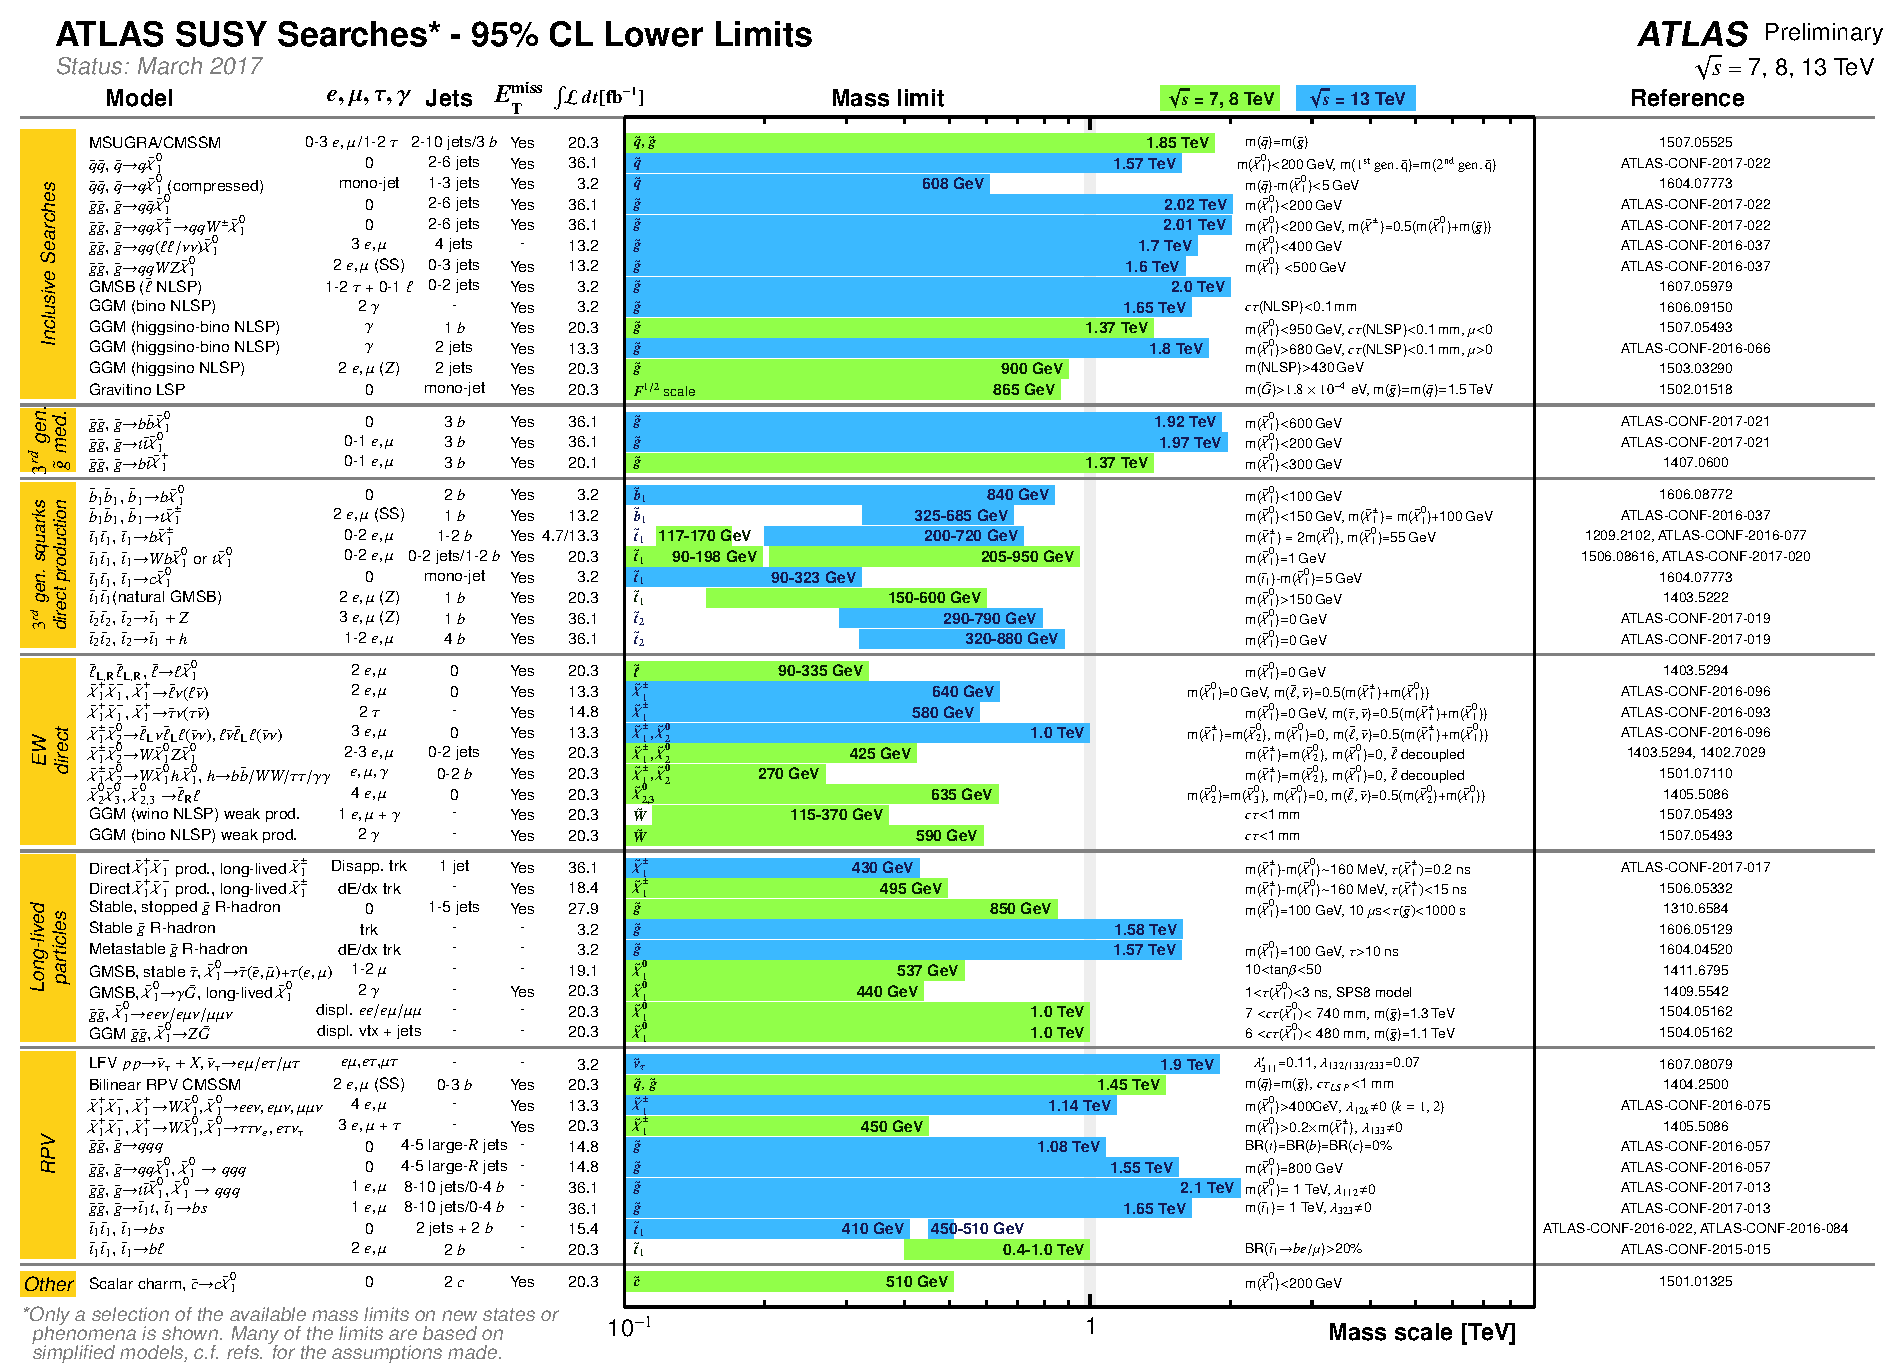
\includegraphics[width=1\textwidth]{masses.pdf}
\caption{Resumen de los límites de exclusión en la masa de las partículas supersimétricas por distintos análisis realizados en ATLAS \cite{masses_web}.}
\label{masses}
\end{figure}



\section{Colisión \textit{pp}}

El LHC es un colisionador de protones, por lo tanto para comprender los procesos que ocurren en el mismo, es necesario entender la estructura del protón. Su composición se puede describir mediante la cromodinámica cuántica (QCD) \cite{ellis1996}, que explica las interacciones entre partículas que poseen carga de color: quarks y gluones. Los mediadores de la interacción, los gluones, pueden interactuar consigno mismo, lo que produce que la fuerza dependa de la distancia entre las cargas. De esta forma, la constante de acoplamiento de la fuerza, aumenta a grandes distancias (o bajas energías) y disminuye para distancias menores (altas energías). Es por este motivo que los cálculos perturbativos solo se pueden efectuar a altas energías. Otra característica de la interacción es el confinamiento, es decir, que las partículas con color no puedan existir libremente. Solo estados de color neutro de múltiples partículas de color pueden ser observados en la naturaleza viajando distancias macroscópicas.

El protón es un barión, compuesto por dos quarks \textit{u} y un quark \textit{d}, cada uno con una carga de color tal que deje al protón en un estado neutro. Estos tres quarks son llamados quarks de valencia del protón, y están rodeados por un mar de gluones y pares de quark-antiquark que surgen de fluctuaciones cuánticas. A altas energías la colisión entre protones se puede considerar como una colisión entre dos de sus constituyentes, aplicando el <<modelo de partones>>. Este modelo fue introducido por Feynman \cite{PhysRevLett.23.1415} y Bjorken \cite{PhysRev.185.1975} a fines de los años 60, para interpretar los resultados de los experimentos de dispersión inelástica profunda (DIS) electrón-nucleón en SLAC. Los quarks de valencia y los quarks y antiquarks del mar junto con los gluones son llamados <<partones>> del protón. Cada partón lleva solo una fracción del momento y la energía del protón. Para la medición de una sección eficaz de dispersión fuerte que involucre quarks y gluones en el estado inicial, es necesario conocer el momento de las partículas incidentes. Como los partones solo llevan una fracción del momento del protón, y están en interacción permanente entre ellos, el momento es desconocido, por lo que la escala de energía de las colisiones varía. Además, como se mencionó, los quarks (\textit{q}) y gluones (\textit{g}) salientes no pueden observarse directamente debido al confinamiento, pero son observados en el detector como jets. Entonces no es posible medir una sección eficaz partónica como $\sigma(qg \rightarrow qg)$, pero se puede hacer una medida inclusiva, como la sección eficaz hadrónica $\sigma(pp \rightarrow jj)$ con dos jets en el estado final. En teoría de perturbaciones, para pasar desde la sección eficaz partónica a la sección eficaz hadrónica es necesario conocer la probabilidad de que un partón de tipo \textit{n} sea encontrado con una fracción de momento \textit{x}, es decir, las funciones de distribución partónica (PDF). Estas funciones son determinadas a partir de datos obtenidos de los propios experimentos de altas energías, ya que no pueden determinarse a partir de la teoría. 

Esta conexión entre los hadrones observables y el nivel partónico es posible gracias al concepto de <<factorización>>, que permite una separación sistemática entre las interacciones de corta distancia (de los partones) y las interacciones de larga distancia (responsables del confinamiento de color y la formación de hadrones). El teorema de factorización \cite{ELLIS1978281} establece que la sección eficaz de producción de cualquier proceso de QCD del tipo $A + B \rightarrow X$, siendo $a_{i}$ ($b_{j}$) los constituyentes del hadrón inicial $A$ ($B$), puede ser expresada como: 

\begin{equation}
\sigma_{AB\rightarrow X}=\sum_{ij}\int dx_{a_{i}}dx_{b_{j}}f_{A/a_{i}}(x_{a_{i}},\mu_{F}^{2})f_{B/b_{j}}(x_{b_{j}},\mu_{F}^{2})\sigma_{a_{i}b_{j}}(\mu_{F}^{2},\mu_{R}^{2})
\end{equation}

\noindent
donde $x_{i}$ ($x_{j}$) es la fracción del momento del hadrón $A$($B$) que lleva el partón $a_{i}$ ($b_{j}$) y $\sigma_{a_{i}b_{j}\rightarrow X}$ es la sección eficaz de la interacción a nivel partónico, calculada a un dado orden de perturbaciones y una escala de renormalización $\mu_R$. La escala de renormalización es introducida para absorber las divergencias ultravioletas que aparecen en los cálculos perturbativos más allá del primer orden. Las funciones $f_{A/a_{i}}(x_{a_{i}},\mu_{F}^{2})$ son las PDF, que representan la probabilidad de encontrar un partón de tipo \textit{n} en el hadrón \textit{h} con una fracción de momento $x_{n}$, dada una escala de factorización $\mu_{F}$. Esta escala es un parámetro arbitrario introducido para tratar singularidades que aparecen en el régimen no perturbativo. Estas divergencias son absorbidas, en forma similar a la renormalización, dentro de las funciones de distribución partónicas a la escala $\mu_{F}$. 


A modo de ejemplo, en la Figura \ref{cross_section}, se muestra el buen acuerdo entre la sección eficaz de algunos procesos del SM medidas por ATLAS y las predicciones teóricas. Las observaciones experimentales realizadas en LHC resultan compatibles con el SM a un nivel de muy alta precisión.


\begin{figure}[ht]
\centering
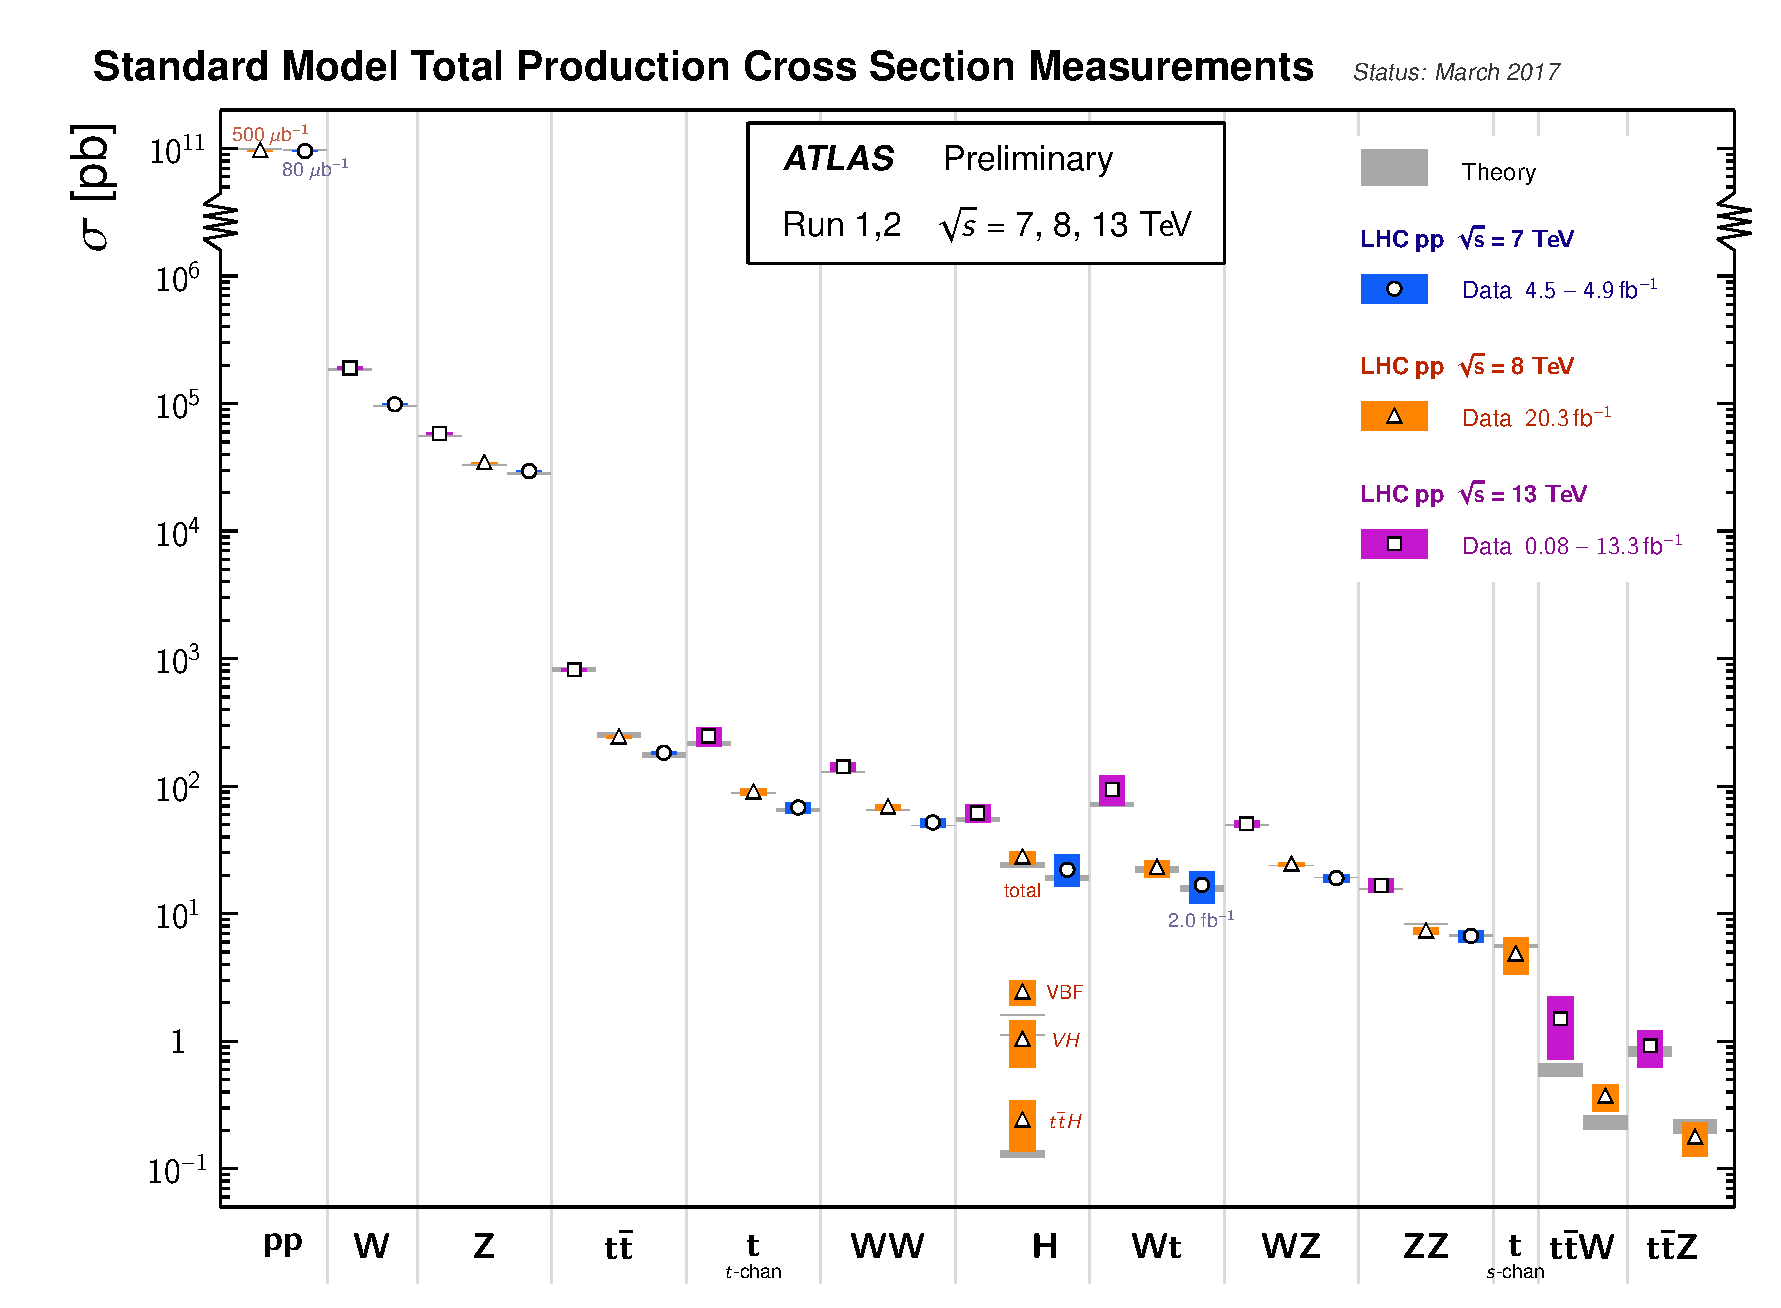
\includegraphics[width=1\textwidth]{cross_section.pdf}
\caption{Resumen de las distintas medidas de sección eficaz de producción de procesos del SM, comparadas con sus valores teóricos esperados \cite{crosssect_web}.}
\label{cross_section}
\end{figure}


\clearpage

\chapter{El LHC y el detector ATLAS}
% \addcontentsline{toc}{chapter}{El LHC y el detector ATLAS}
\chaptermark{El LHC y el detector ATLAS}



El Gran Colisionador de Hadrones (\textit{\textbf{L}arge \textbf{H}adron \textbf{C}olider} (LHC)) \cite{Evans:1129806} es el acelerador de hadrones de la Organización Europea para la Investigación Nuclear (CERN, por sus antiguas siglas en francés), ubicado en la frontera entre Francia y Suiza. Posee una longitud de 27 km y fue construido en el mismo túnel en el que funcionaba el acelerador $e^{+}e^{-}$ LEP (entre 1989 y 2000) \cite{LEPbook}, a una profundidad variable entre $50$ y $174$ m de la superficie.

El LHC está diseñado para colisionar protones (e iones pesados) a una energía de centro de masa de $\sqrt{s}=14 \etev$. Para ello el CERN posee un complejo de aceleradores que, en sucesivas etapas, incrementan la energía de los protones (Figura \ref{acc_complex}). El último de los aceleradores es el LHC, donde los protones circulan en direcciones opuestas por cavidades de ultra alto vacío a una presión de $10^{-10}$ torr. El mismo cuenta con $1232$ dipolos magnéticos superconductores enfriados a $1.9$ K, que generan un campo magnético de $8.4$ T, lo que permite mantener en su órbita circular a los protones. Los dipolos están equipados con sextupolos, octupolos y decapolos, que permiten corregir las pequeñas imperfecciones del campo magnético en las extremidades de los dipolos. Para aumentar la probabilidad de colisión, existe un sistema de focalización de los haces en las proximidades de los detectores, que estrecha el camino que recorren los protones. El mismo consiste de $392$ cuadrupolos magnéticos que generan campos magnéticos de $6.8$ T. 

\begin{figure}
\centering
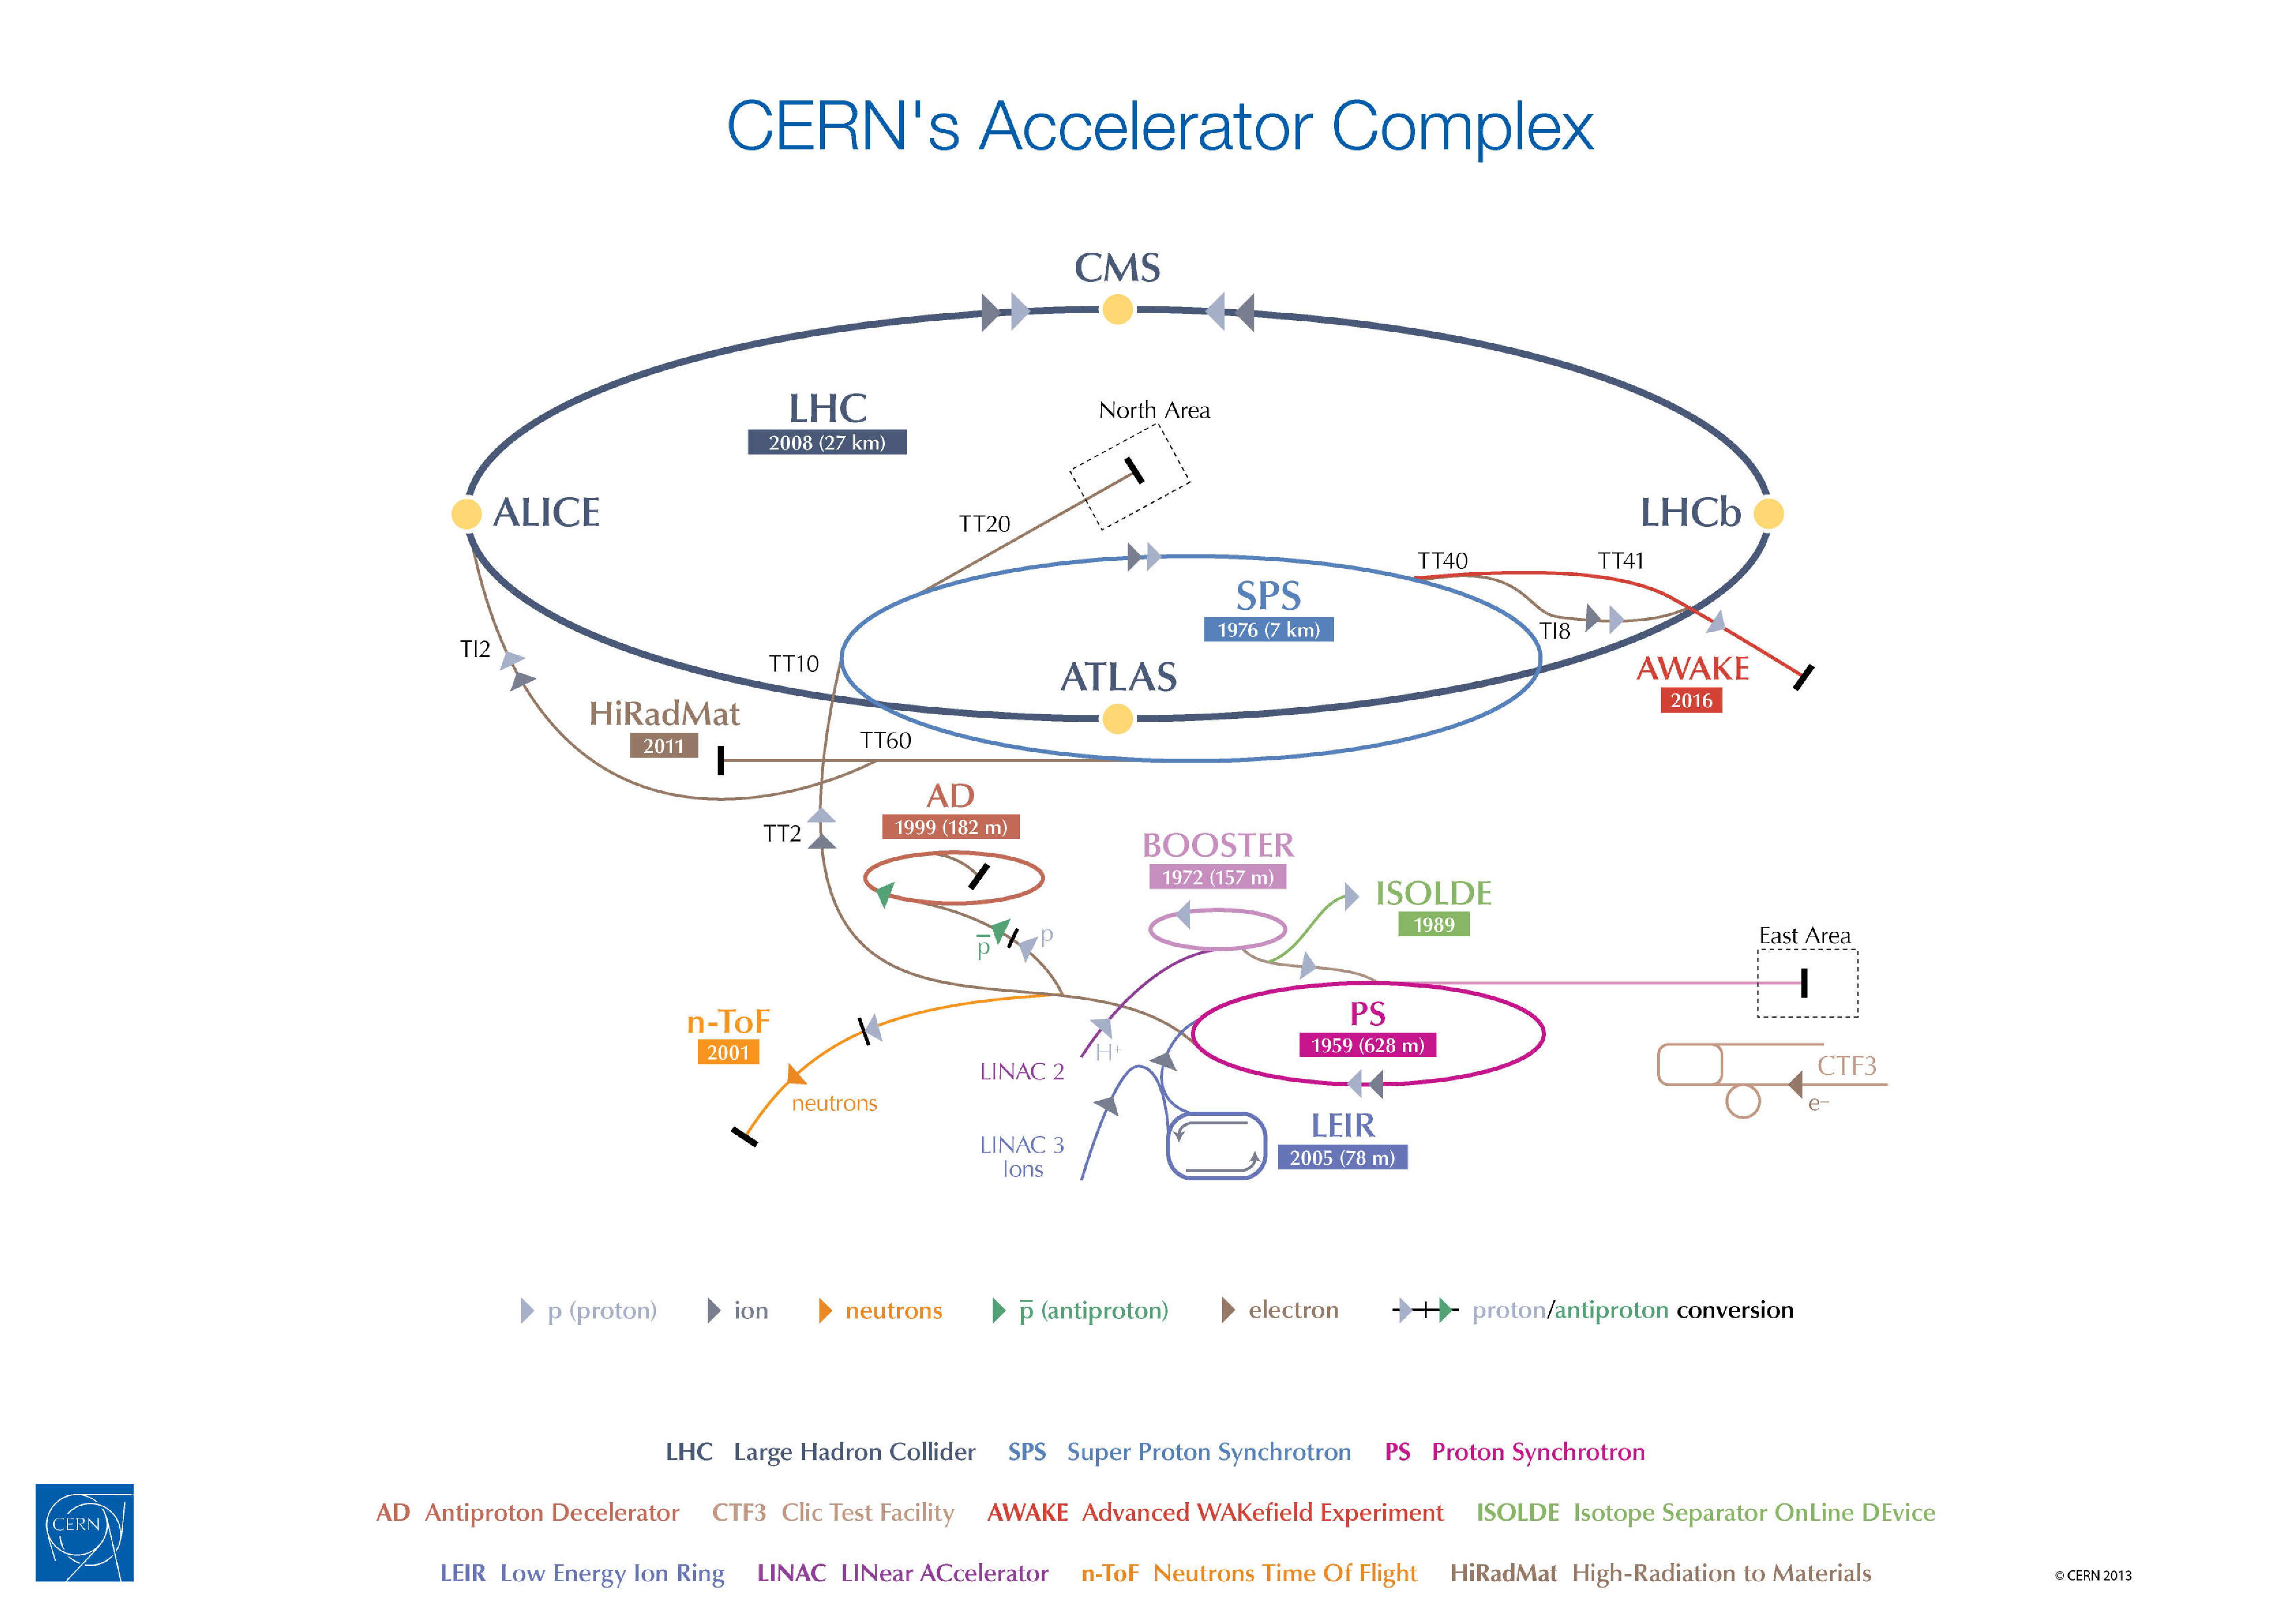
\includegraphics[width=1\textwidth]{acc_complex-eps-converted-to.pdf}
\caption{Complejo de aceleradores del CERN, incluyendo al LHC y a la serie de aceleradores utilizados para proveer de protones al LHC. También pueden verse los diferentes experimentos ubicados en distintos puntos del acelerador.}
\label{acc_complex}
\end{figure}

El diseño del LHC contempla trenes de $2808$ paquetes de $\sim 10^{11}$ protones cada uno, espaciados temporalmente en $25$ ns. Para caracterizar el funcionamiento del acelerador, se utiliza una variable denominada luminosidad instantánea. Se define como el número de partículas por unidad de tiempo y unidad de área:

\begin{equation}
\mathcal{L}=f_{rev}n_{b}\frac{N_{1}N_{2}}{A}
\end{equation}
% comentario intencional para eliminar sangría
donde $f_{rev}$ es la frecuencia de revolución ($\sim$11 kHz), $n_{b}$ es el número de \textit{bunches} (paquetes de protones) por haz, $N_{i}$ es el número de partículas en cada \textit{bunch} y \textit{A} es la sección efectiva del haz, que puede expresarse en término de los parámetros del acelerador como:

\begin{equation}
A=\frac{4 \pi \epsilon_{n}\beta^{*}}{\gamma F}
\end{equation}
% comentario intencional para eliminar sangría
donde $\epsilon_{n}$ es la emitancia transversal normalizada (la dispersión transversal media de las partículas del  haz en el espacio de coordenadas e impulsos), $\beta^{*}$ es la función de amplitud en el punto de interacción, relacionada al poder de focalización de los cuadrupolos), $\gamma$ es el factor relativista de Lorentz y \textit{F} es un factor de reducción geométrico, debido al ángulo de cruce de los haces en el punto de interacción.


El LHC funciona desde 2009, pero entre 2013 y 2014 no estuvo operativo debido a que se le hicieron remodelaciones para mejorar su desempeño. En el 2015 volvió a funcionar (Run 2), alcanzando una energía por haz de $6.6 \etev$ ($13 \etev$) y una luminosidad de $1.4\cdot 10^{34}$ cm$^{-2}$s$^{-1}$.

\section{El detector ATLAS}

ATLAS (\textit{\textbf{A} \textbf{T}oroidal \textbf{L}HC \textbf{A}paratu\textbf{S}})  \cite{PERF-2007-01} es uno de los experimentos multipropósito del LHC, diseñado para estudiar las colisiones protón-protón a altas energías provistas por el LHC.

El esquema del detector se puede observar en la Figura \ref{ATLAS}. Tiene una simetría aproximadamente cilíndrica, y está compuesto de distintos subdetectores, que cumplen diversas funciones en la identificación de las partículas producidas durante las colisiones (ver Figura \ref{cross_section_2}). En la zona más próxima al haz se encuentra detector interno de trazas (ID), compuesto del Insertable B-Layer (IBL), un detector de píxeles, un detector de bandas de silicio (SCT) y un detector de radiación de transición (TRT). Envolviendo el ID se encuentra un solenoide superconductor que genera un campo magnético de $2$ T, el cual curva la trayectoria de las partículas cargadas para así medir su impulso.

\begin{figure}
\centering
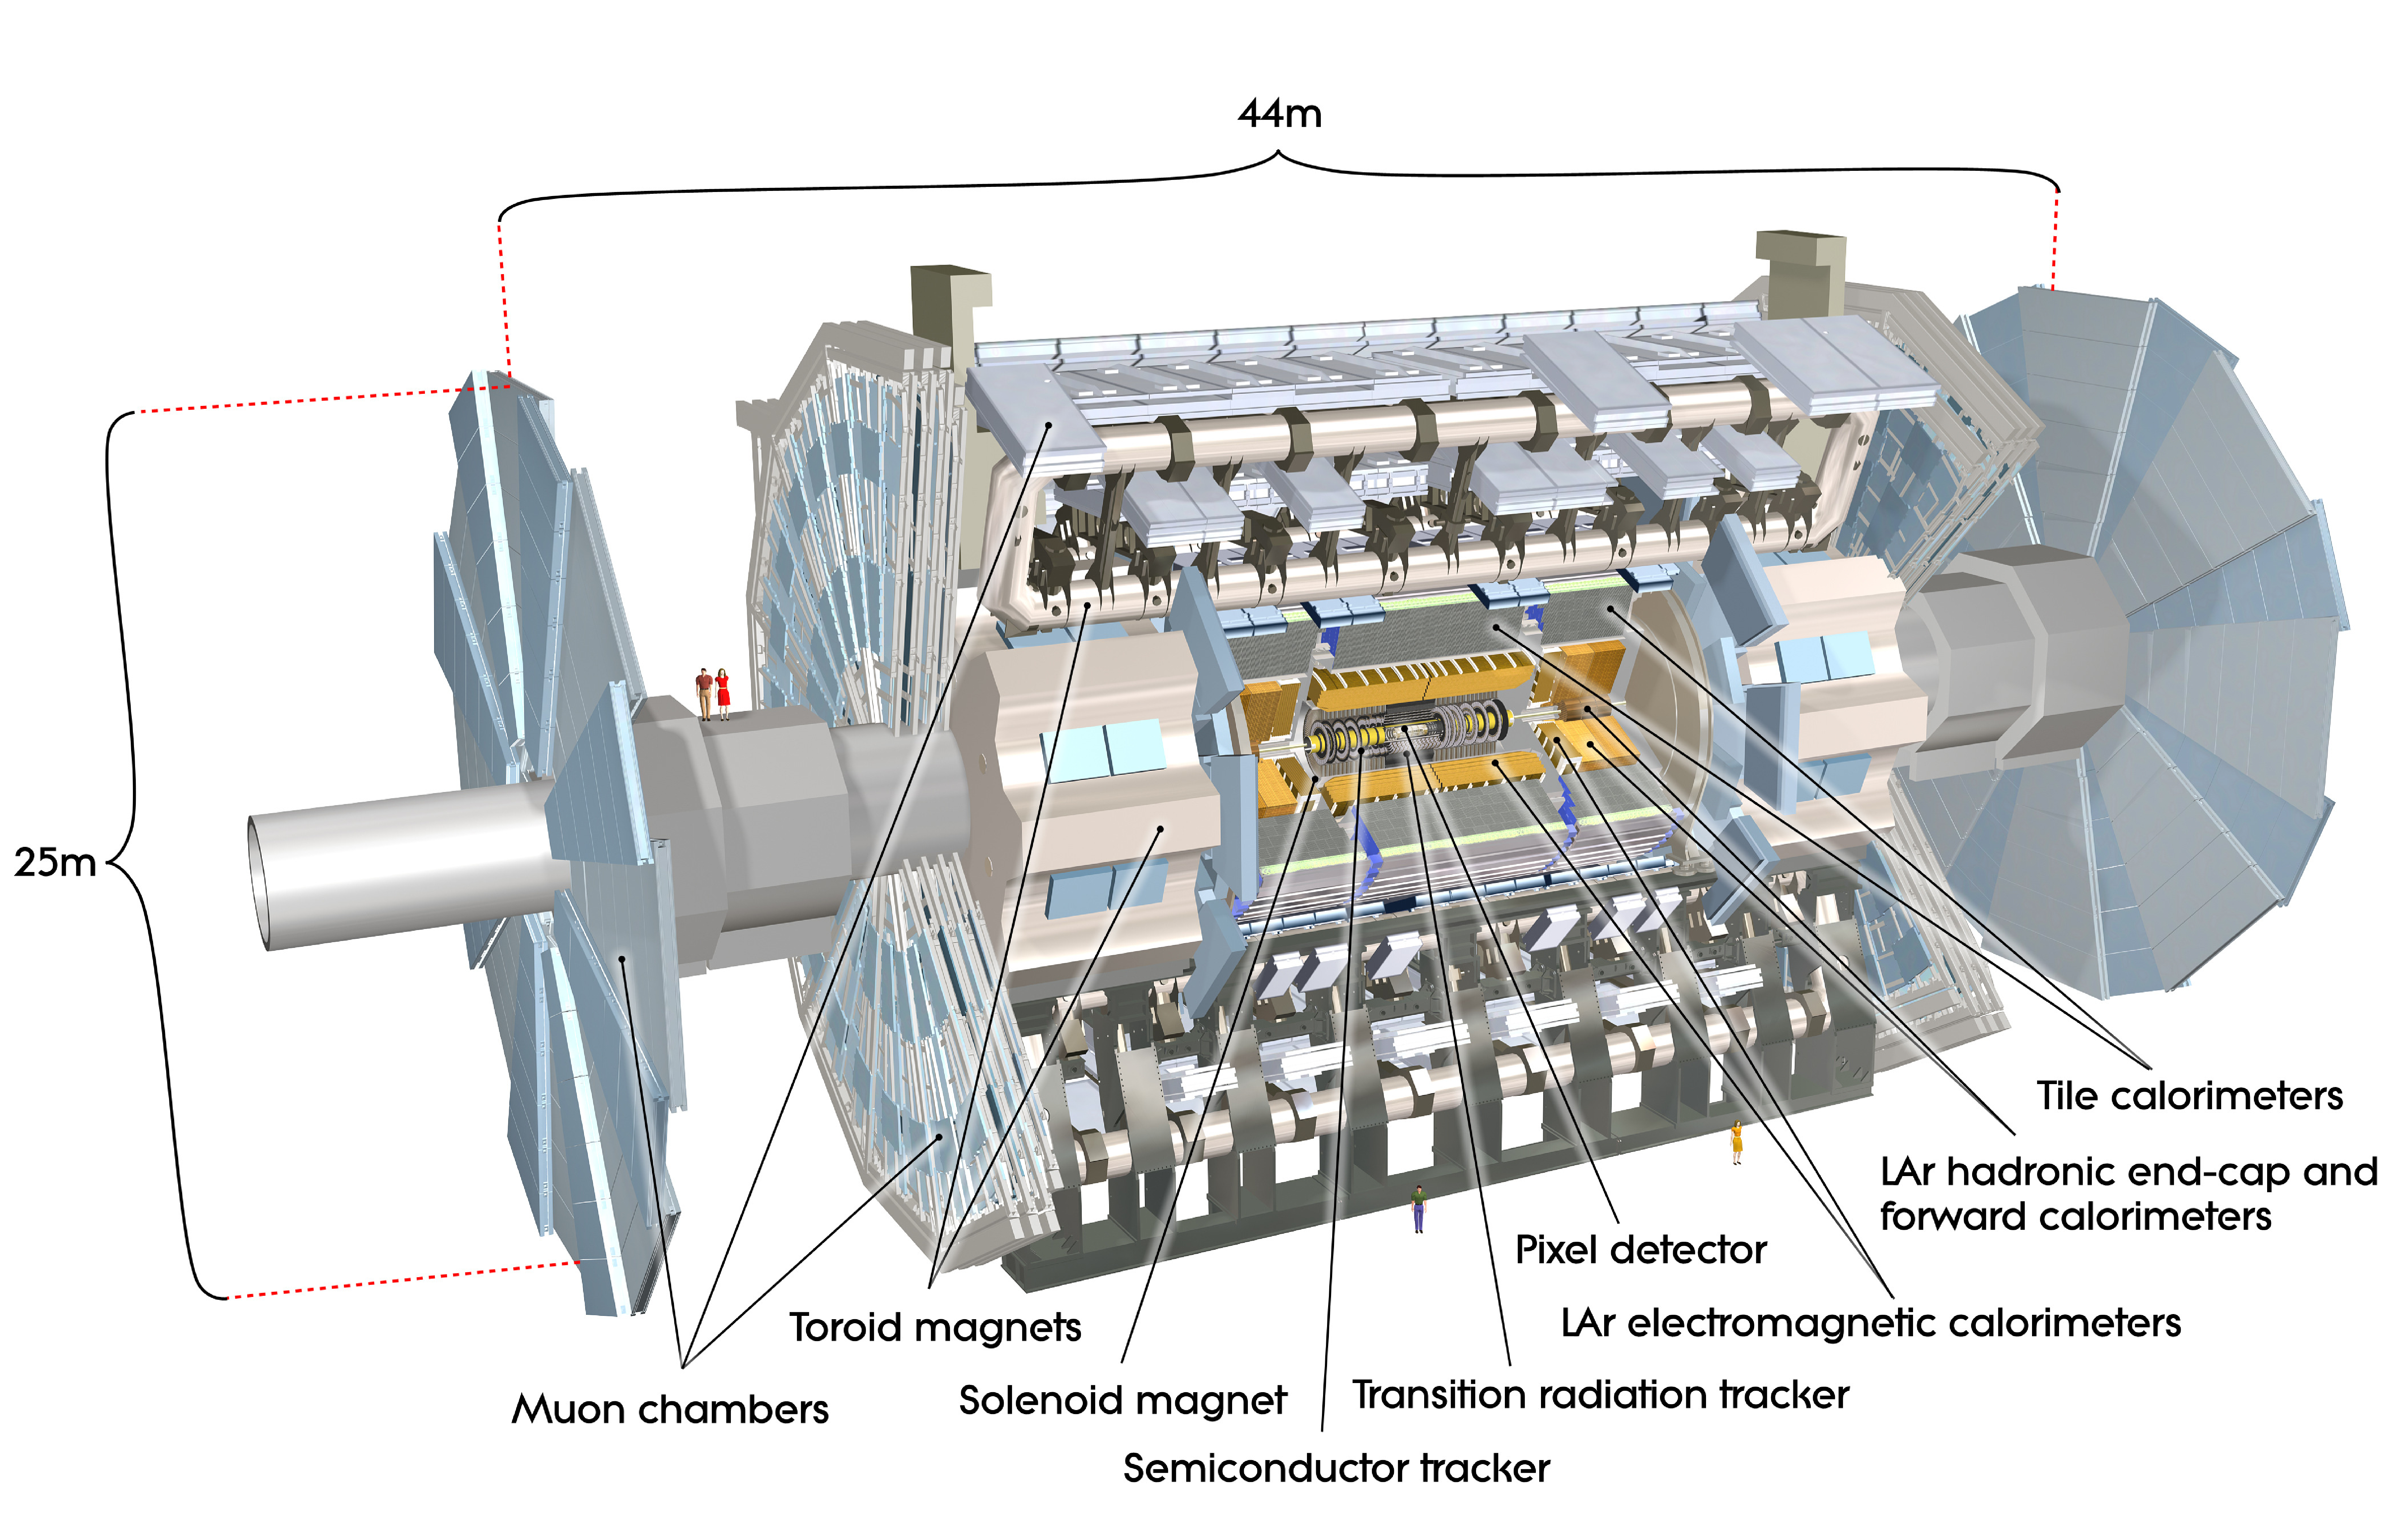
\includegraphics[width=1\textwidth]{ATLAS-eps-converted-to.pdf}
\caption{Esquema general del detector de ATLAS.}
\label{ATLAS}
\end{figure}

\begin{figure}
\centering
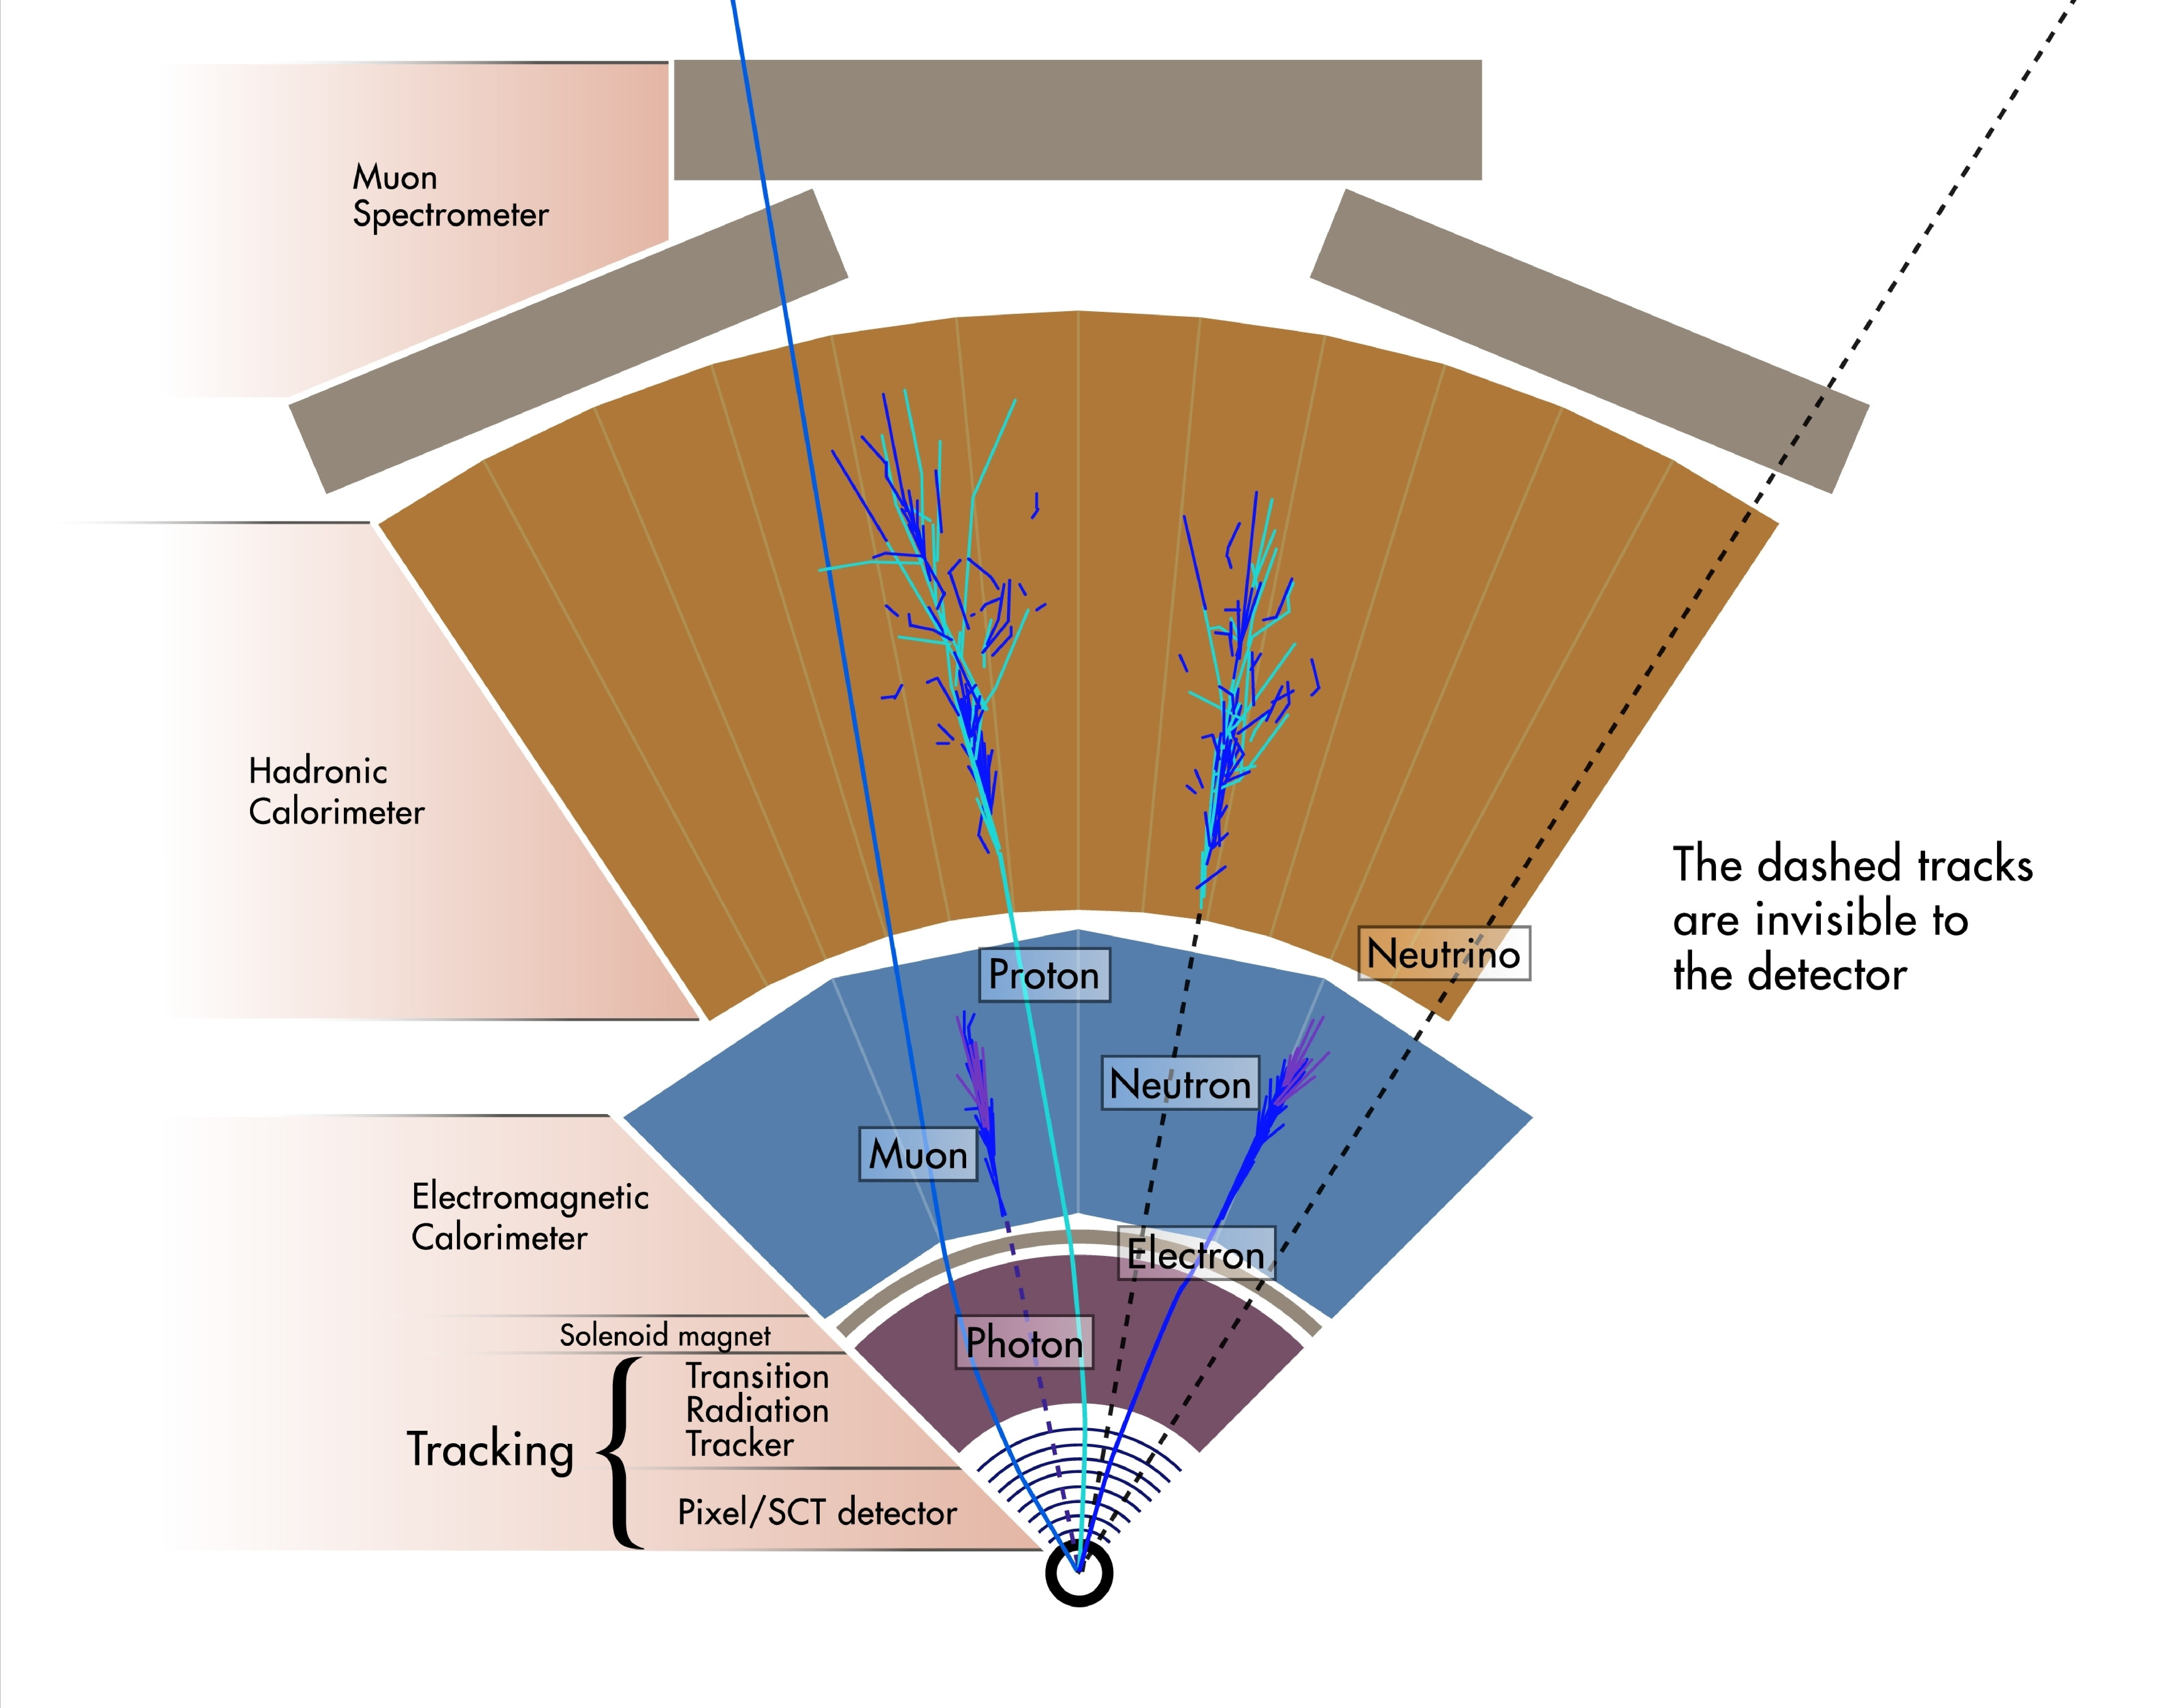
\includegraphics[width=0.7\textwidth]{cross_section_2-eps-converted-to.pdf}
\caption{Esquema del corte transversal del detector de ATLAS, ilustrando los distintos subdetectores y el pasaje de los distintos tipos de partículas.}
\label{cross_section_2}
\end{figure}

A continuación se ubica el sistema de calorímetros: el calorímetro electromagnético (ECAL) que mide principalmente la energía depositada por fotones y electrones, y el calorímetro hadrónico (HCAL) para medir la energía de los jets y hadrones.

Finalmente, se encuentra el espectrómetro de muones (MS), que le da a ATLAS un tamaño total de $45$ m de largo y $25$ m de alto. Intercalado con este, se encuentra un sistema de imanes toroidales, que generan un campo magnético de $4$ T para curvar la trayectoria de los muones hacia el final del detector.

El detector ATLAS se divide geométricamente en dos regiones, la parte central denominada \textit{barrel} y la región extrema \textit{endcap}. En la región \textit{barrel} los detectores se ubican en forma de cilindros concéntricos alrededor del eje del haz, mientras en la región \textit{endcap} se disponen como discos perpendiculares a la dirección del haz. 

\section{Sistema de coordenadas}

El sistema de coordenadas de ATLAS corresponde a un sistema cartesiano, cuyo origen coincide con el punto de interacción nominal. El eje \textit{z} corresponde al eje del haz, el eje \textit{x} se define desde el punto de interacción hacia el centro del LHC, y el eje \textit{y} se define apuntando hacia arriba.

Es conveniente además definir un sistema de coordenadas cilíndricas. Donde el radio \textit{R} representa la distancia perpendicular al haz. El ángulo azimutal $\phi$ es medido alrededor del eje del haz, y el ángulo $\theta$ se mide con respecto al eje del haz. 

Una cantidad muy importante utilizada en física de altas energías es la llamada rapidez:

\begin{equation}
w=\frac{1}{2}\ln\left( \frac{E+p_{z}}{E-p_{z}}\right)
\end{equation}
% comentario intencional para eliminar sangría
donde \textit{E} es la energía total de la partícula y $p_{z}$ es la componente longitudinal de su impulso. En el límite de altas energías esta cantidad se aproxima (en forma exacta para partículas no masivas) por la llamada pseudorapidez, $\eta$, relacionada con el ángulo polar $\theta$ como:

\begin{equation}
\eta =-\ln \tan\left( \frac{\theta}{2} \right)
\end{equation}

La razón detrás de esta transformación de coordenadas es el hecho que la multiplicidad de partículas producidas es aproximadamente constante como función de $\eta$, y que la diferencia de pseudorapidez entre dos partículas es invariante frente a transformaciones de Lorentz a lo largo de la dirección del haz. 

En el caso de colisiones hadrónicas, la fracción del impulso del protón adquirida por cada uno de las partones interactuantes es desconocida. Parte de este impulso es transferido en la interacción dura, mientras cierta fracción remanente escapa el detector a lo largo del haz. Así, no es posible reconstruir el movimiento longitudinal del centro de masa en la interacción, y aplicar leyes de conservación sobre la cinemática de cada evento. Sin embargo, dado que los protones inciden a lo largo de la dirección del haz, y asumiendo que el momento transverso de los partones es nulo, el impulso total transverso se conserva durante la colisión. Por esta razón, solo las componentes transversales son utilizadas en la descripción de la cinemática del evento, por ejemplo $p_{T}$ ($=p\sin\theta$). En términos de la pseudorapidez, se define la energía transversa ($E_{T}=E\sin\theta$) de una partícula como:

\begin{equation}
E_{T}=\frac{E}{\cosh \eta}
\end{equation}
% comentario intencional para eliminar sangría
donde \textit{E} es su energía total.

\section{Los subdetectores de ATLAS}

\subsection{El detector interno}

\begin{figure}
\centering
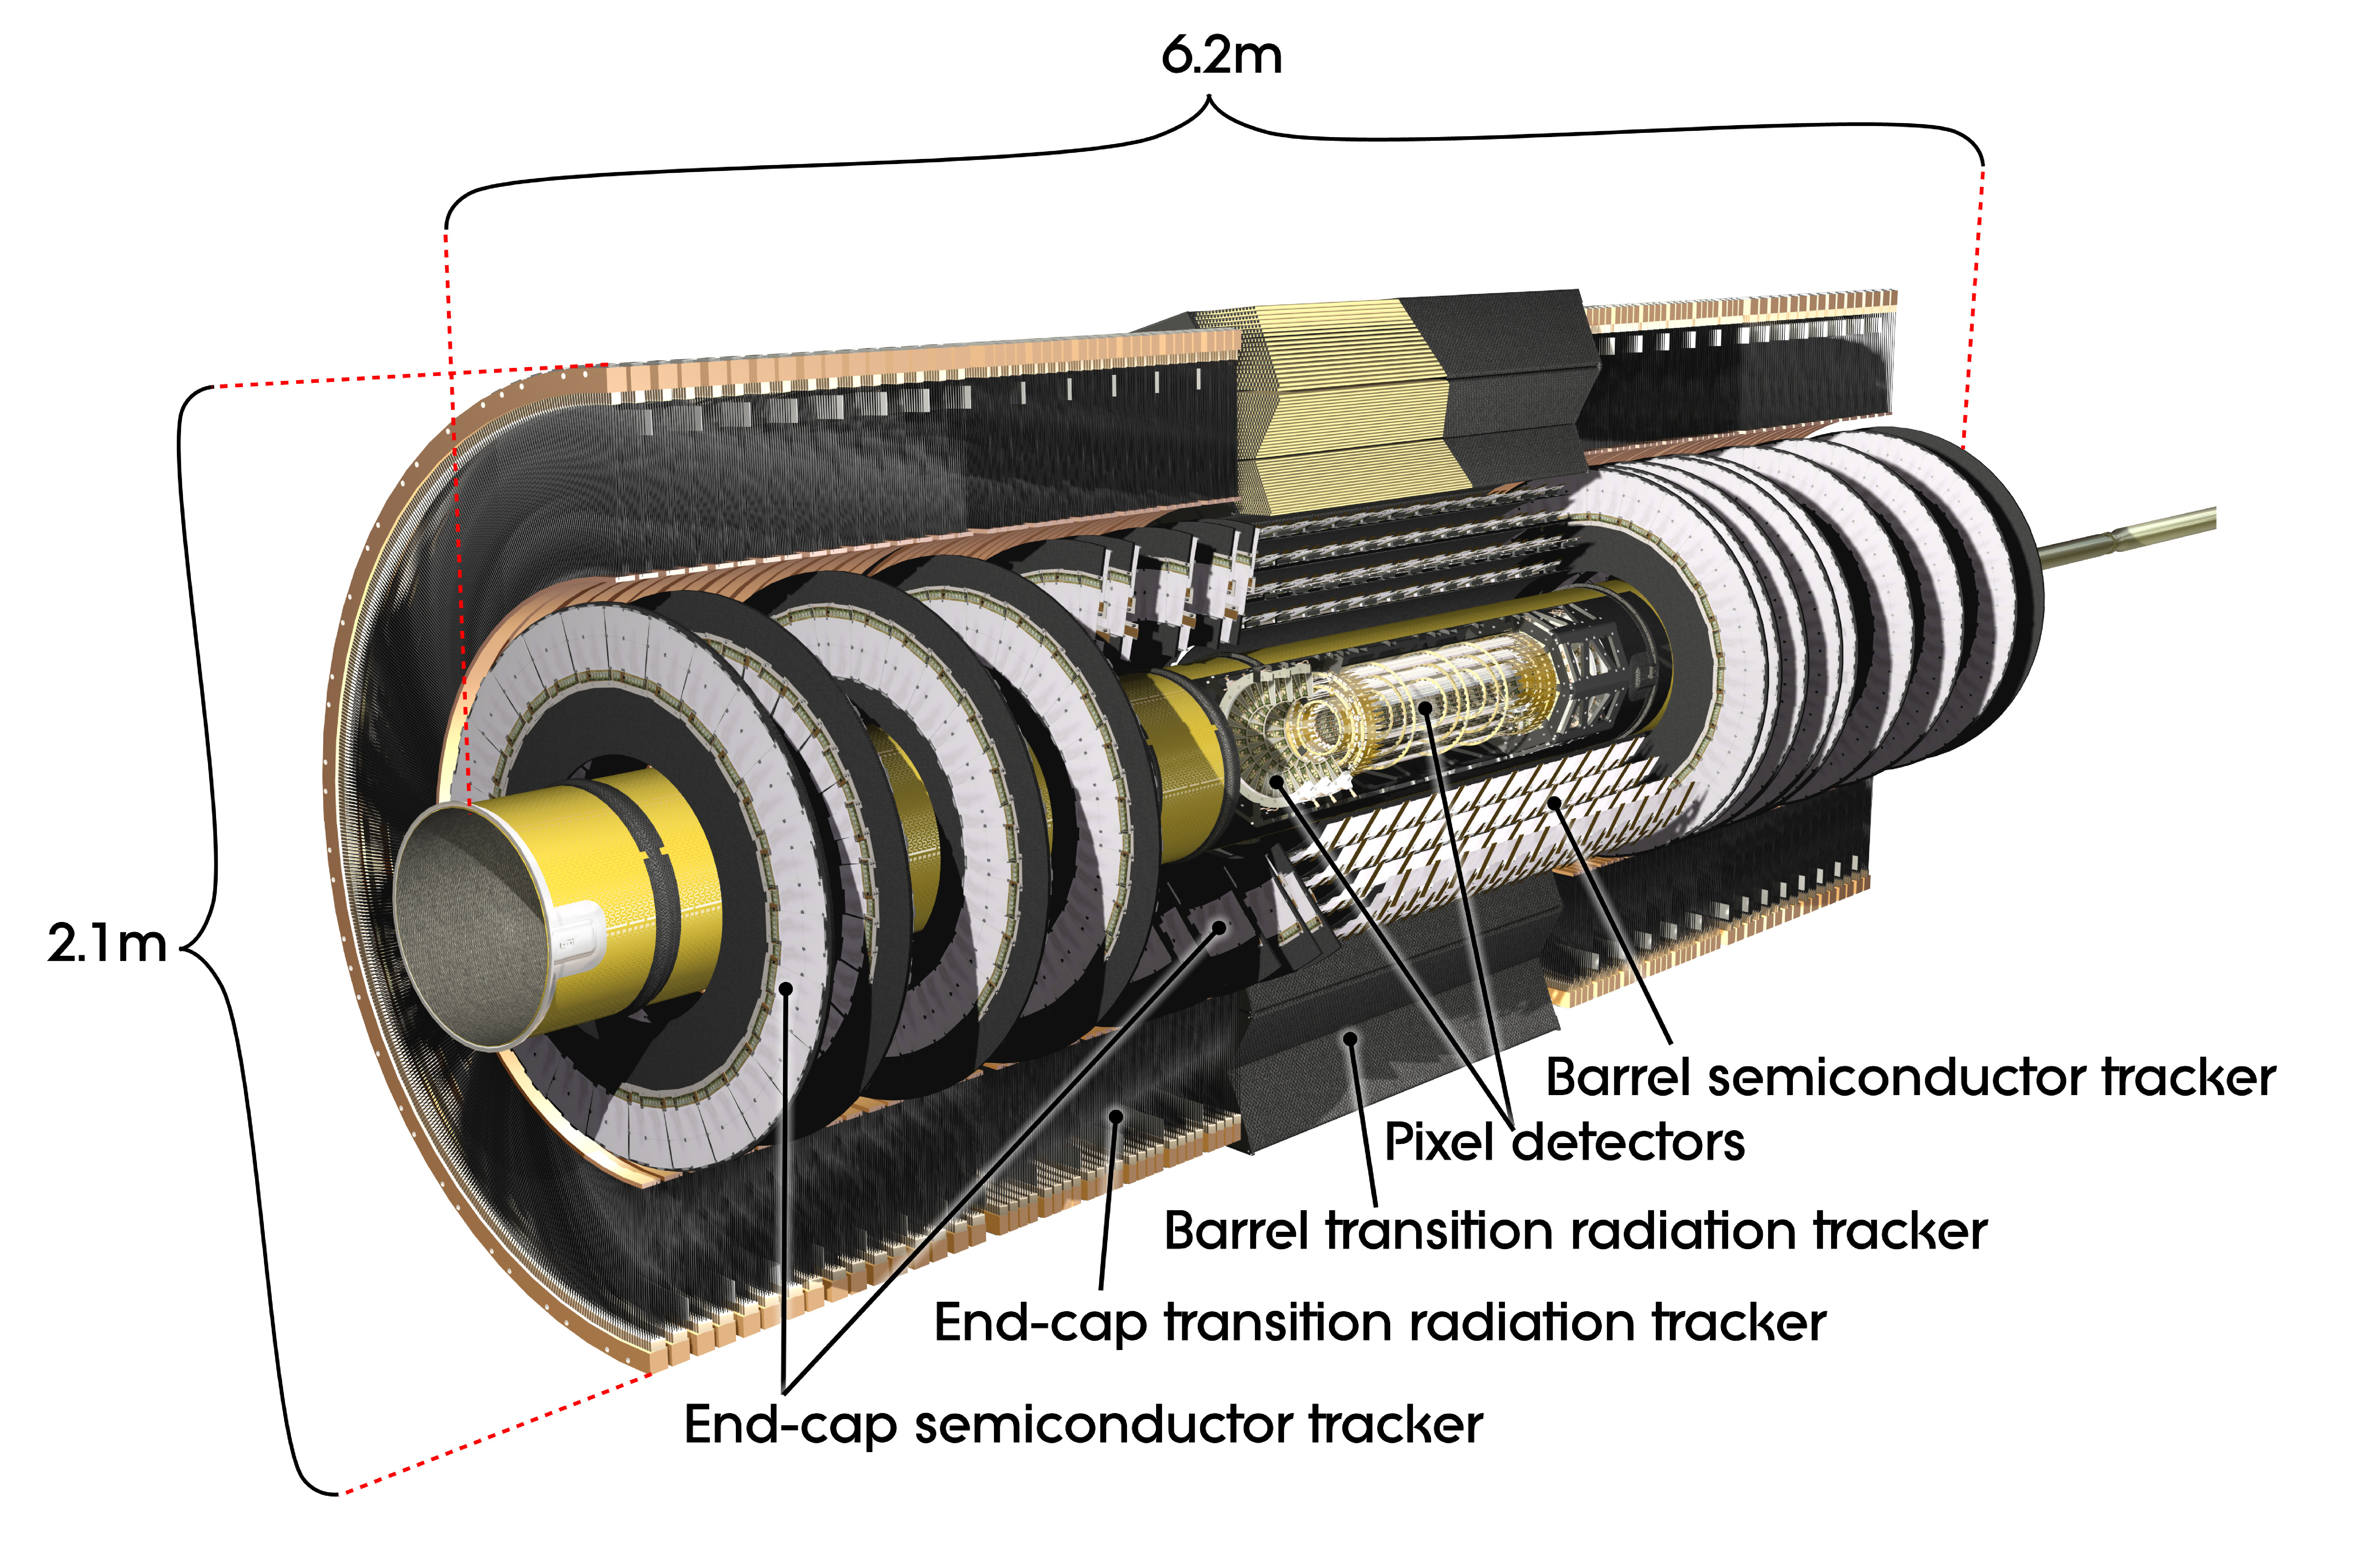
\includegraphics[width=0.70\textwidth]{ID-eps-converted-to.pdf}
\caption{Esquema general del detector interno de ATLAS.}
\label{ID}
\end{figure}

El detector interno (Figura \ref{ID}) es el más próximo al haz y combina detectores de muy alta resolución con detectores continuos de trazas. Está contenido dentro del solenoide que provee un campo magnético de $2$ T. Los distintos detectores que lo componen se describen a continuación. Se puede ver un corte transversal de los mismos en la Figura \ref{ID_2}.

\begin{figure}
\centering
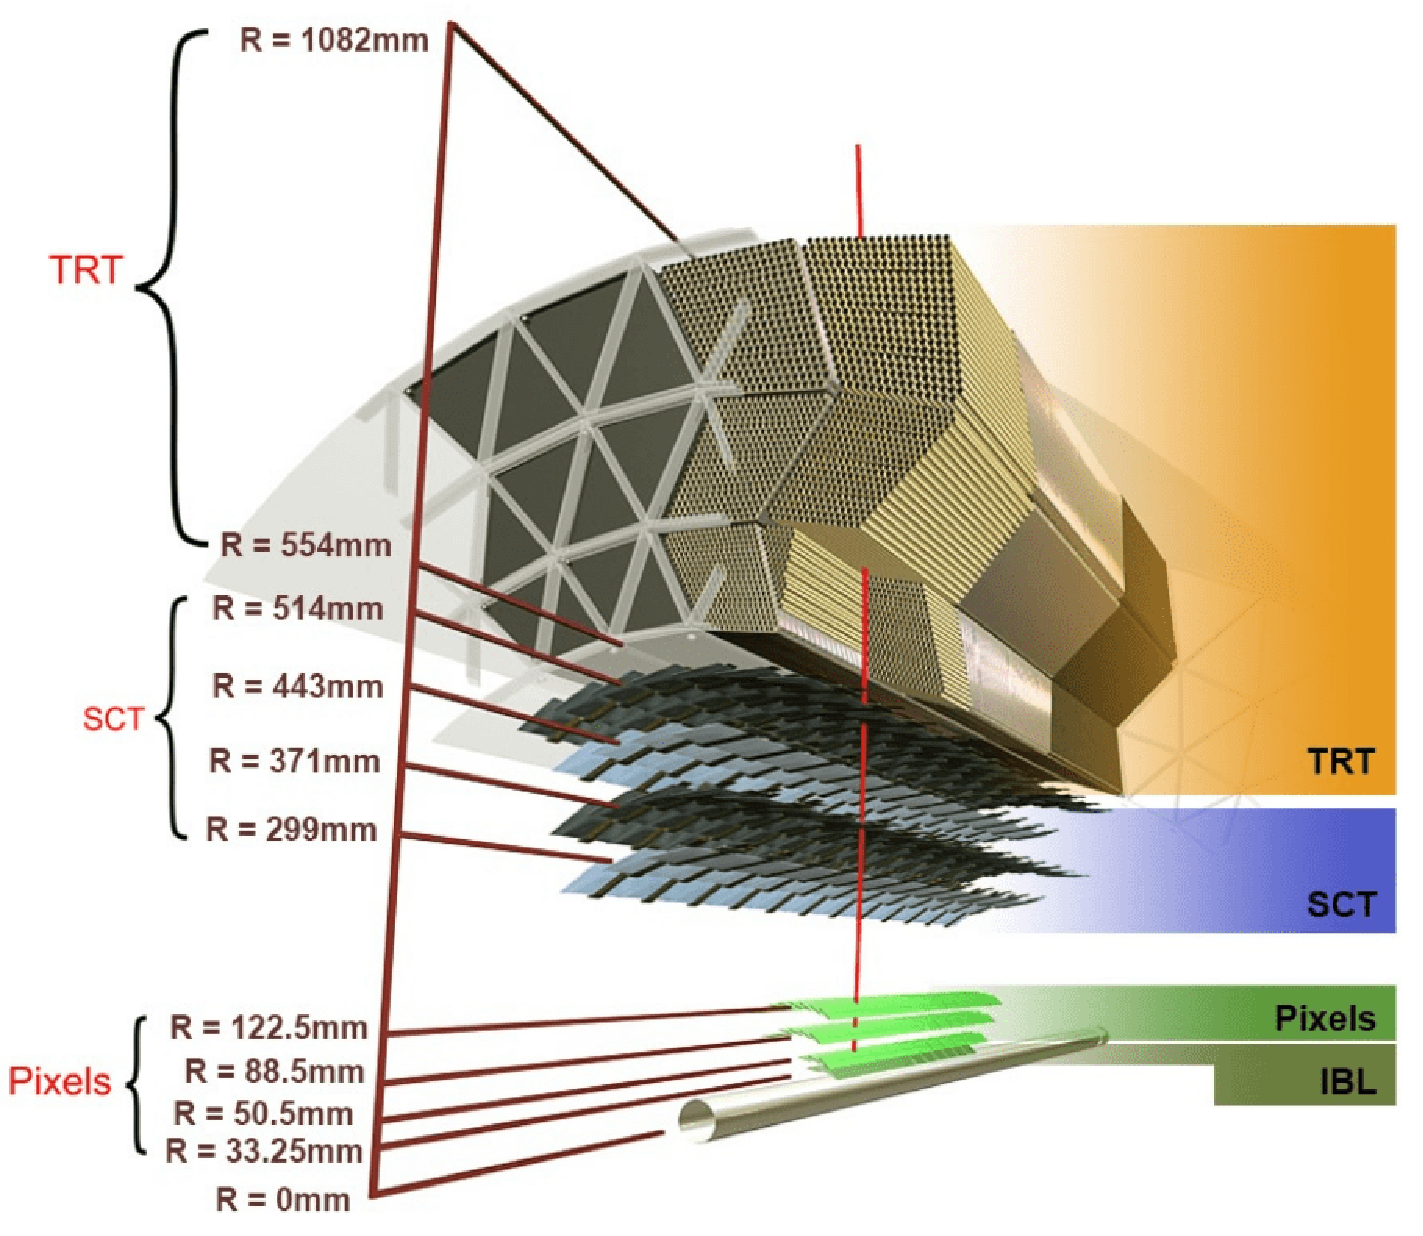
\includegraphics[width=0.60\textwidth]{ID_2.pdf}
\caption{Esquema del detector interno mostrando la traza de una partícula cargada de $p_{T}=10 \egev$ atravesándolo. La trayectoria atraviesa el tubo del haz de  berilio, las tres capas del detector de píxeles de silicio, las cuatro capas dobles del SCT, y aproximadamente 36 tubos contenidos en los módulos del TRT.}
\label{ID_2}
\end{figure}
% \vspace{0.5cm}

\subsubsection{Insertable B-Layer}

Luego del Run 1 la luminosidad del LHC aumentó notablemente, lo que podía significar un daño por radiación en los detectores internos. En vez de reemplazar las partes del detector de píxeles que podían ser dañadas, se decidió colocar una capa insertable entre el detector de píxeles y la tubería donde circulan los protones. El objetivo del mismo es mejorar la eficiencia en la identificación de trazas, vértices, y en la identifiación de bottom quarks, que decaen típicamente fuera del radio del IBL.

El IBL está compuesto por $8$ millones de chips de rápida lectura y con sensores de silicio, que detectan el paso de partículas cargadas mediante la deposición de carga inducida. El tamaño de los píxeles es de $50\times250\:\mu$m$^{2}$, con una resolución de $8\:\mu$m ($R-\phi$) y $40\:\mu$m ($z$). La distancia entre el IBL y la tubería es de $0.2$ mm, y entre el tubo y el detector de píxeles es de $1.9$ mm. 

\subsubsection{Detector de píxeles}

El detector de píxeles fue construido para medir la posición de las trazas de partículas cargadas con la más alta precisión posible y es de vital importancia para la reconstrucción de los vértices primarios y secundarios. En la región \textit{barrel} el detector se compone de tres capas cilíndricas, mientras que la \textit{endcap} de tres discos. La capa más interna, denominada \textit{B-Layer}, se encuentra a $50.5$ mm del punto de interacción. El principio de detección para partículas cargadas es la medida de la deposición de la carga inducida en una capa de silicio por ionización. El sistema contiene un total de $80$ millones de sensores, cada uno con una resolución de $10\:\mu$m ($R-\phi$) y $115\:\mu$m ($z$).

\subsubsection{Detector Semiconductor de Trazas (SCT)}

Se encuentra por fuera del detector de píxeles y está diseñado para medir las trazas con alta precisión en la zona intermedia del detector. A diferencia del detector de píxeles, estos sensores de silicio están segmentados en micro bandas, dada la más baja multiplicidad de partículas. La resolución de $17\:\mu$m ($R-\phi$) y $580\:\mu$m ($z$). En la región \textit{barrel} los módulos de SCT están dispuestos en 4 capas concéntricas, mientras que en la región \textit{endcap} consiste en 9 discos transversales al eje del haz.

\subsubsection{Detector de Radiación de Transición (TRT)}

Es el detector más externo del ID y está diseñado, no solo para detectar partículas cargadas, sino también para distinguir entre partículas pesadas y livianas. El TRT se compone de tubos detectores de $4$ mm de diámetro, con un gas que ioniza al ser atravesado por partículas cargadas. Los electrones producidos son colectados por una ánodo, y el tiempo de deriva es una medida de la distancia a la traza del mismo.  Además, los tubos están rodeados de fibras de polipropileno con un índice de refracción diferente, por lo que las partículas que atraviesan el detector emiten radiación con una intensidad proporcional a $\gamma=E/m$. De esta forma, el TRT permite distinguir partículas cargadas pesadas ($\pi^{\pm}$) de aquellas más livianas ($e^{\pm}$). La región \textit{barrel} contiene $50000$ tubos paralelos al eje del haz y la región \textit{endcap} $320000$ tubos orientados radialmente. Su resolución es de $0.17$ mm.

\subsection{Calorímetros}

El sistema de calorímetros de ATLAS está diseñado para medir la energía y la posición de las partículas, mediante la absorción de la energía depositada por las cascadas de partículas secundarias que estas generan en el material del mismo. Además, permite discriminar electrones y fotones de jets, medir el desbalance de energía transversa y la selección online de eventos potencialmente interesantes (\textit{trigger}). Este sistema incluye un calorímetro electromagnético (ECAL) y otro hadrónico (HCAL), como muestra la Figura \ref{Cal}.

\begin{figure}
\centering
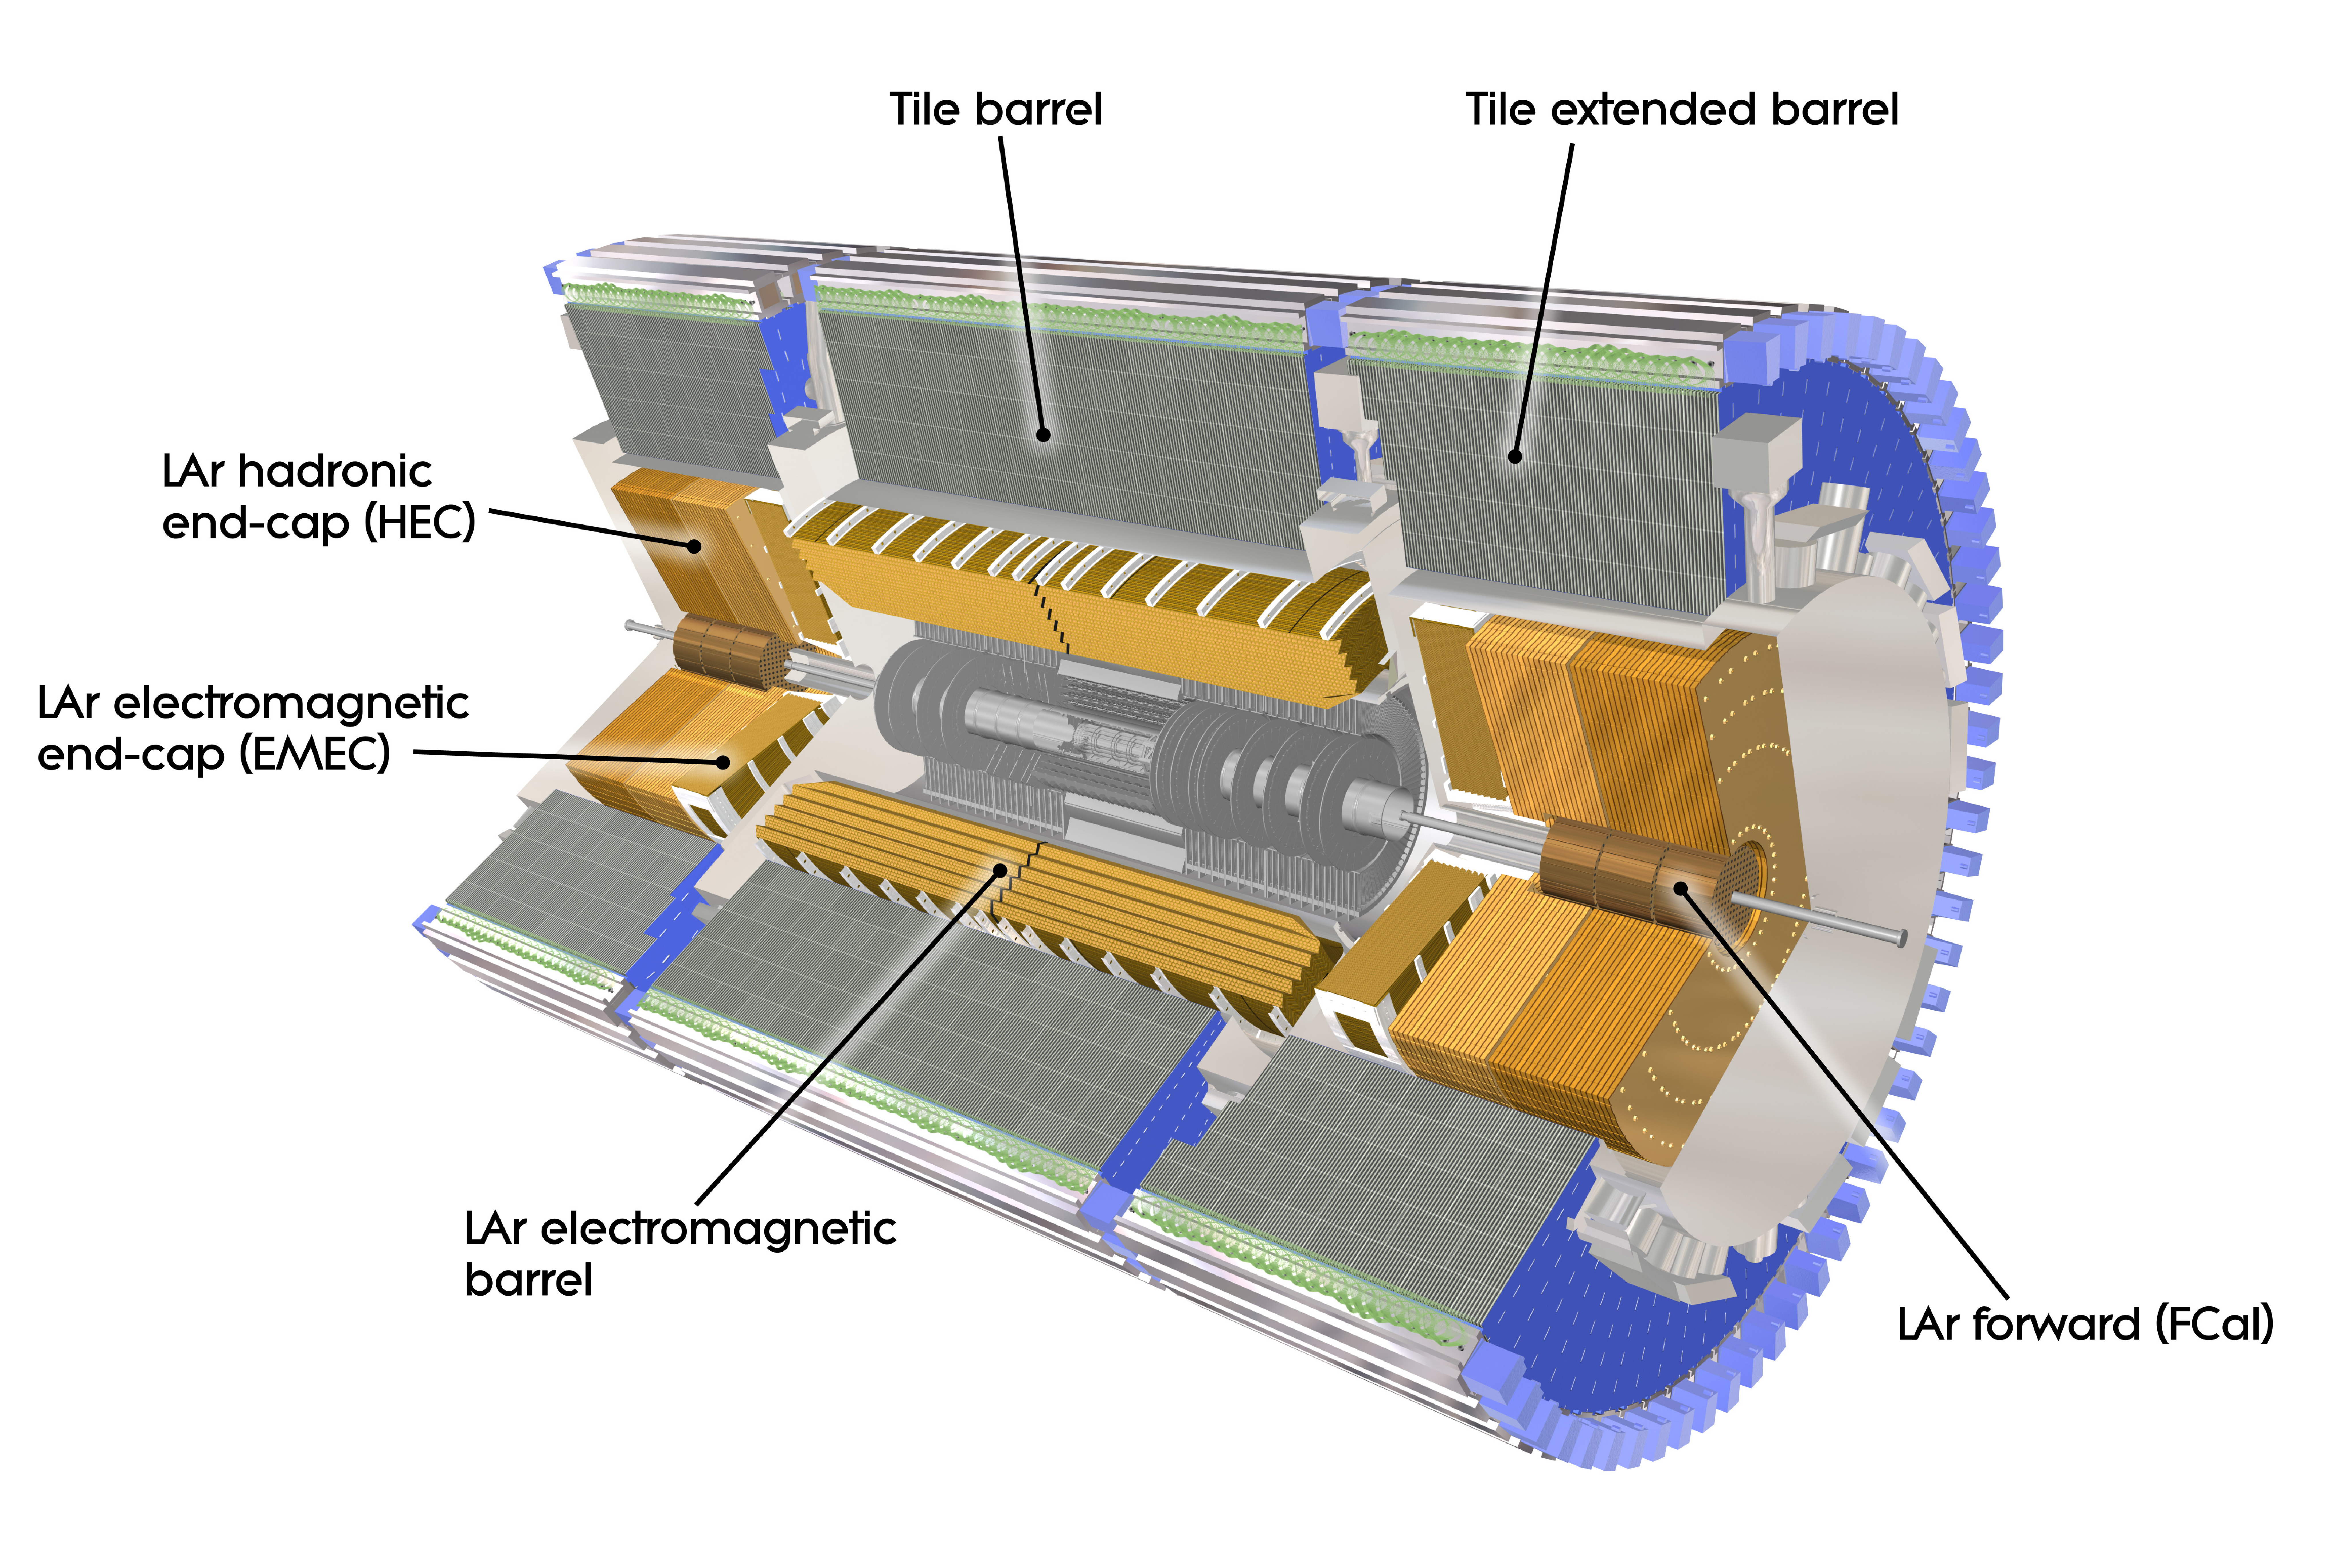
\includegraphics[width=0.70\textwidth]{Cal-eps-converted-to.pdf}
\caption{Sistema de calorímetros del detector ATLAS.}
% \vspace{0.2cm}\footnotesize\textbf \sl{...}\vspace{0.2cm}
\label{Cal}
\end{figure}

\subsubsection{Calorímetro electromagnético (ECAL)}

El ECAL en un calorímetros de muestreo inhomogéneo no compensado, que utiliza plomo como material absorbente. Las partículas incidentes interactúan con este material creando una lluvia de partículas cargadas y neutras. Las partículas cargadas ionizan el medio activo (LAr) colocado entre las placas de plomo, donde los electrones liberados son colectados en un electrodo central de kaptón/Cu hacia donde derivan por acción del campo eléctrico aplicado. La señal total en el medio activo es así proporcional a la energía total real de la partícula incidente.

% \begin{figure}
% \centering
% 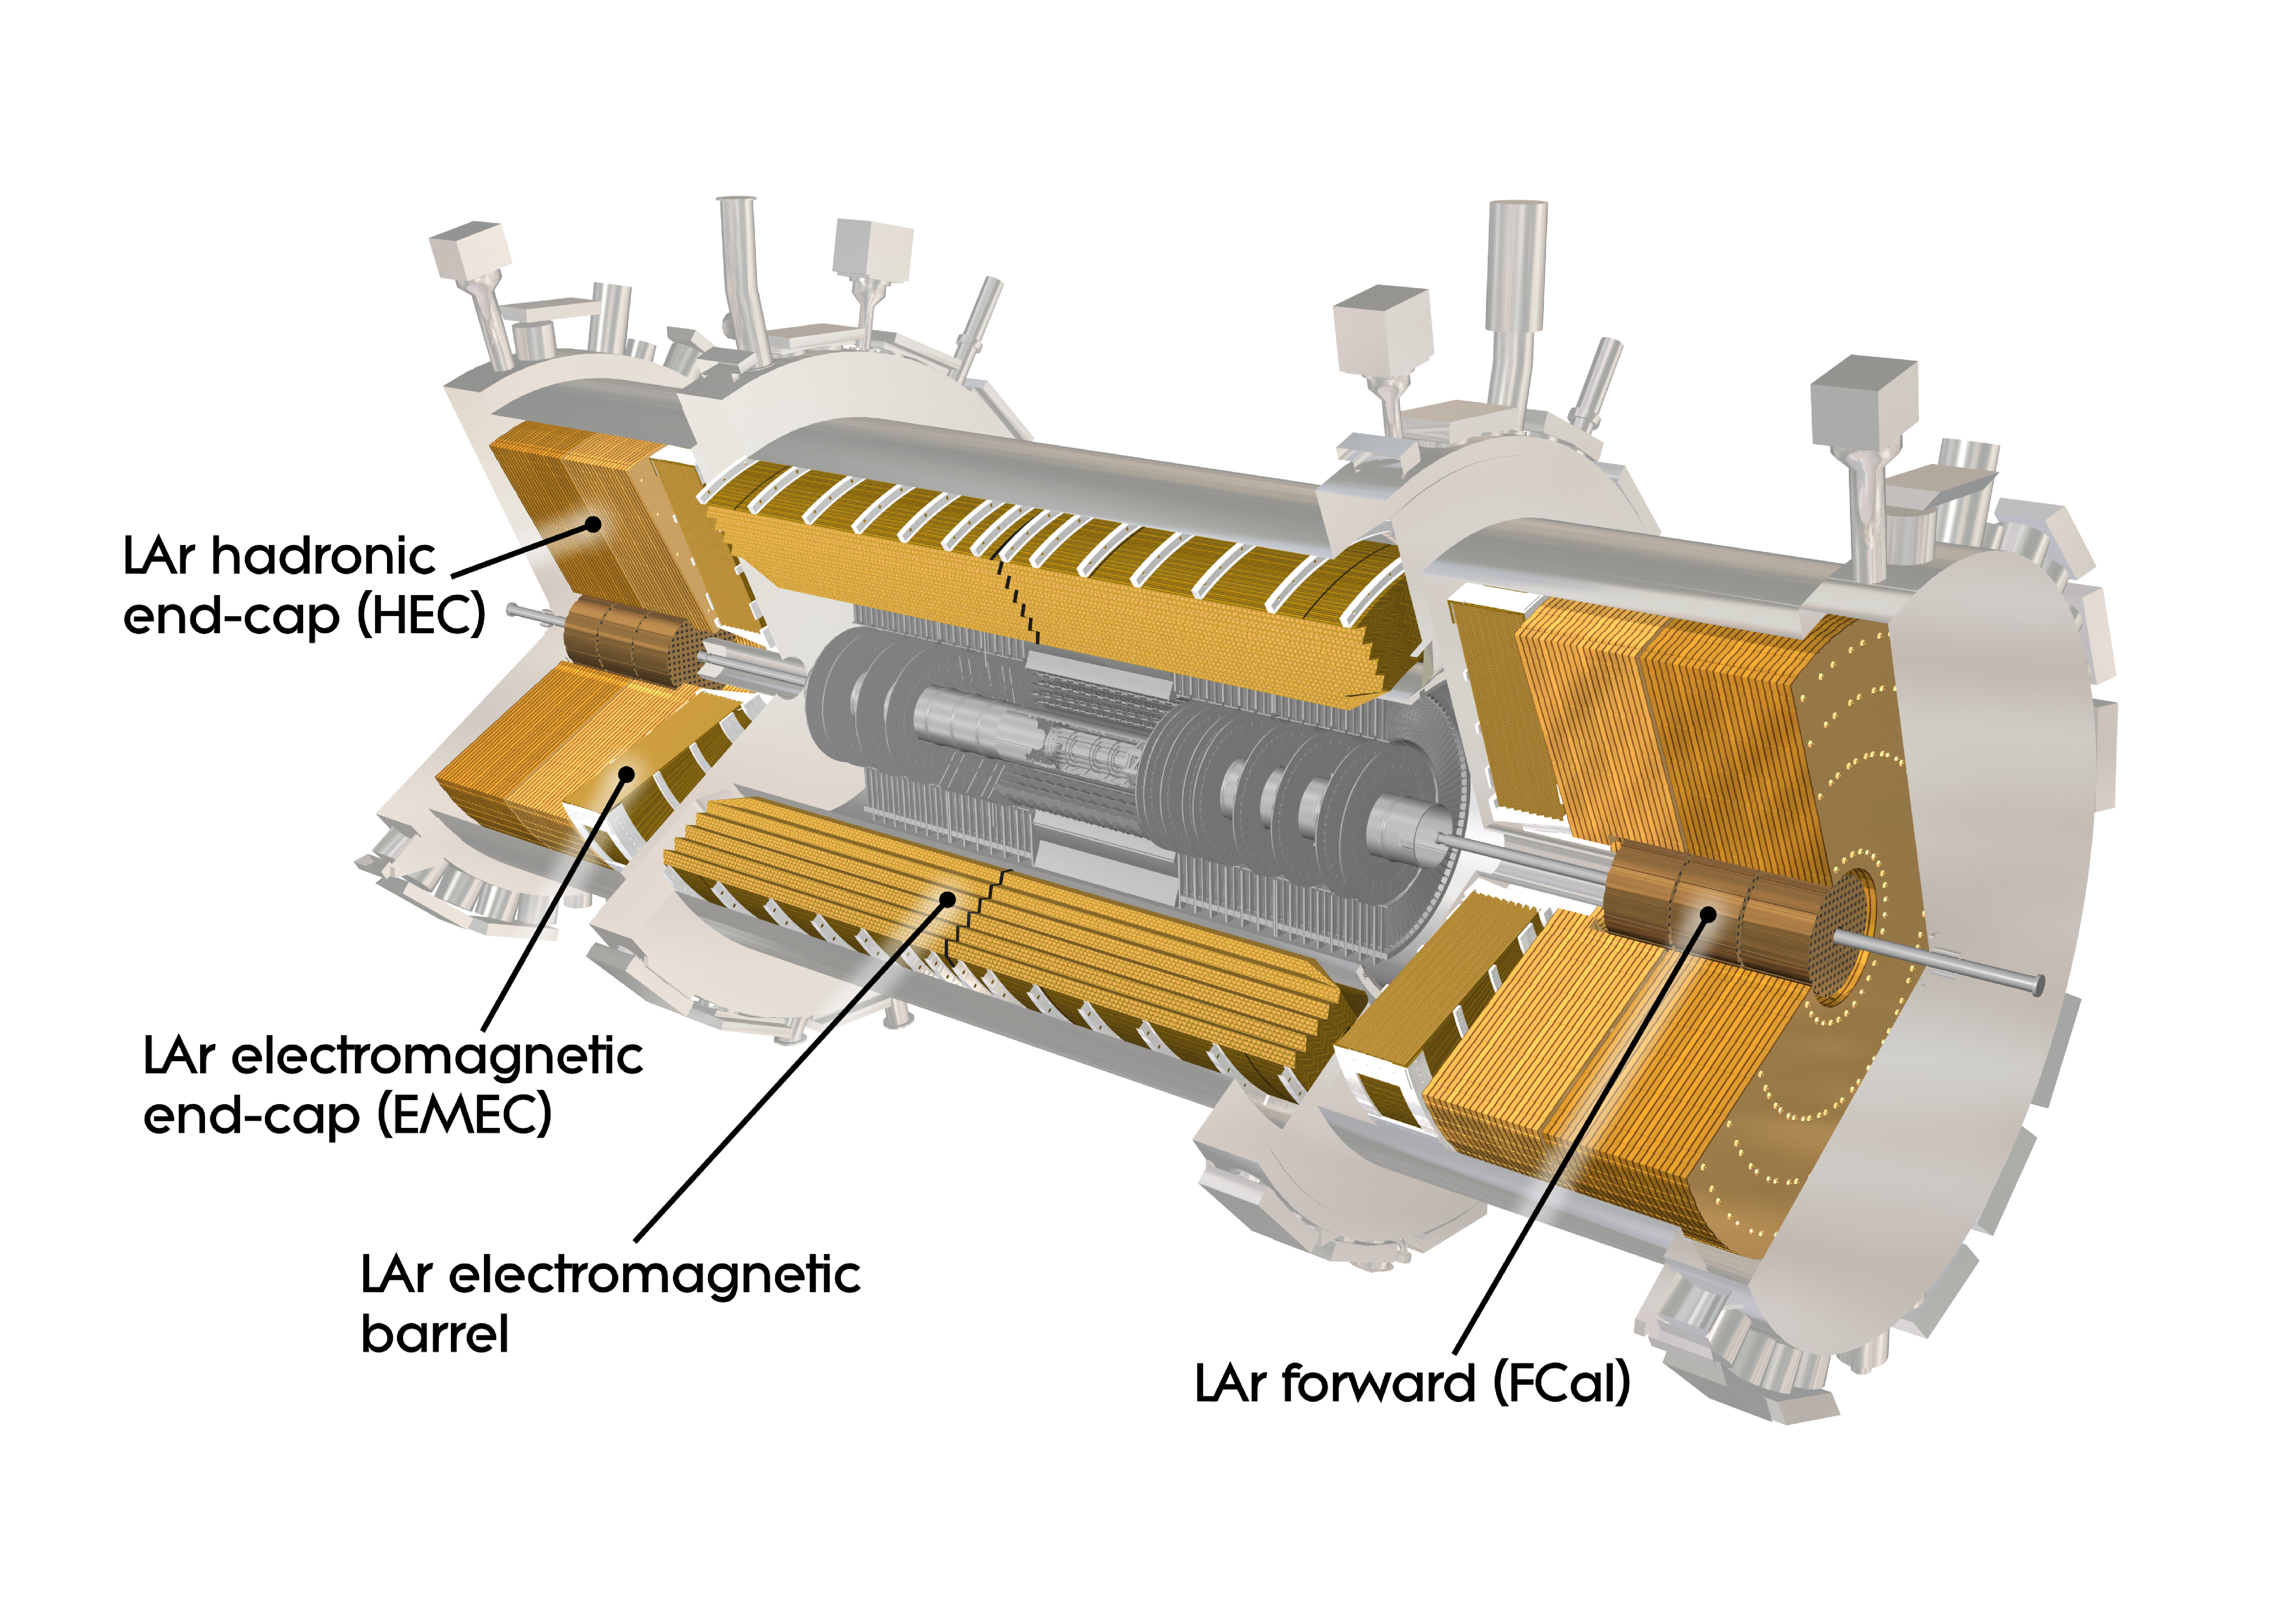
\includegraphics[width=0.70\textwidth]{ecal.eps}
% \caption{ECAL del detector ATLAS.}
% % \vspace{0.2cm}\footnotesize\textbf \sl{...}\vspace{0.2cm}
% \label{ecal}
% \end{figure}

El ECAL se divide en una parte central (\textit{barrel}) y dos \textit{endcaps} a cada lado. En la región de transición entre el \textit{barrel} y el \textit{endcap} se encuentra una zona no instrumentada, por donde se conecta el detector. Esta región, denominada \textit{crack}, está comprendida entre $1.37 < |\eta| < 1.52$. Es por este motivo que la mayoría de los análisis se requiere que los candidatos a fotones/electrones estén fuera de la región \textit{crack}.

\subsubsection{Calorímetro hadrónico (HCAL)}

El HCAL es un conjunto de calorímetros que rodean al ECAL. El primero de los calorímetros se denomina \textit{Tile Calorimeter}, es un calorímetro de muestreo que utiliza acero como material absorbente y tejas centelladoras plásticas como material activo. En la región \textit{endcap} se encuentra un calorímetro hadrónico de muestreo (HEC) con placas de cobre como absorbente y argón líquido como material activo, que consiste en dos ruedas, una atrás de la otra. Finalmente se encuentra el Forward Calorimeter (FCAL), un calorímetro de muestreo que extiende la cobertura del sistema a $|\eta|<4.9$. Estos detectores extienden la aceptancia del calorímetro de ATLAS hasta cubrir prácticamente la totalidad de ángulo sólido del punto de colisión.

% El calorímetro hadrónico cubre el rango $|\eta|< 4.9$ usando diferentes materiales. La parte del \textit{barrel} de este sistema utiliza acero como absorbente y tejas centelladoras como material activo. Las tejas están ubicadas radialmente y apiladas en profundidad. En la región de \textit{endcaps}, el calorímetro hadrónico se compone de dos ruedas perpendiculares al tubo del haz, hechas con placas de cobre y tungsteno como material absorbente y argón líquido como material activo. Estos detectores extienden la aceptancia del calorímetro de ATLAS hasta cubrir prácticamente la totalidad de ángulo sólido del punto de colisión.

\subsection{Espectrómetro de muones (MS)}

Los muones de alto $p_{T}$ generados en el punto de interacción tienen un altísimo poder de penetración y son poco interactuantes. Por ello el espectrómetro de muones se encuentra situado en la parte más exterior del detector ATLAS, siendo los muones las únicas partículas que llegan a él. Se encuentra alrededor del sistema de imanes de toroides, y está diseñado para obtener mediciones de alta precisión de la posición e impulso de los muones, y para una rápida identificación para el sistema de \textit{trigger}. Este es el subdetector más grande y el que le da a ATLAS su tamaño característico. 

El MS se compone de diferentes tipos de cámaras de detección de muones (ver Figura \ref{muon}). Las \textit{Monitored Drift Tubes} (MDTs) son responsables de la mayoría de las medidas de precisión. Funcionan de forma similar al TRT, con tubos llenos de un gas que ioniza y un ánodo central que recoge los electrones producidos, y el tiempo de deriva se asocia con la distancia a la traza. En la región \textit{endcap} se encuentran las \textit{Cathode Strip Chambers} (CSCs) que poseen alta resolución espacio-temporal. Estas cámaras funcionan midiendo la carga depositada en un ánodo, producto de la cascada de electrones creados cerca del mismo. Las \textit{Resistive Plate Chamber} (RPCs) proveen una estimación rápida del momento de los muones al primer nivel del \textit{trigger}. Las RPCs miden la descarga ocasionada entre dos placas resistivas paralelas sometidas a una alta diferencia de potencial, tras la ionización del volumen de gas interno causada por el paso de muones energéticos. Finalmente se encuentra las \textit{Thin Gap Chambers} (TGCs), similares en funcionamiento a las CSCs. Se encuentran en la región \textit{endcap} y proveen también información al sistema de \textit{trigger} en esta región.


\begin{figure}
\centering
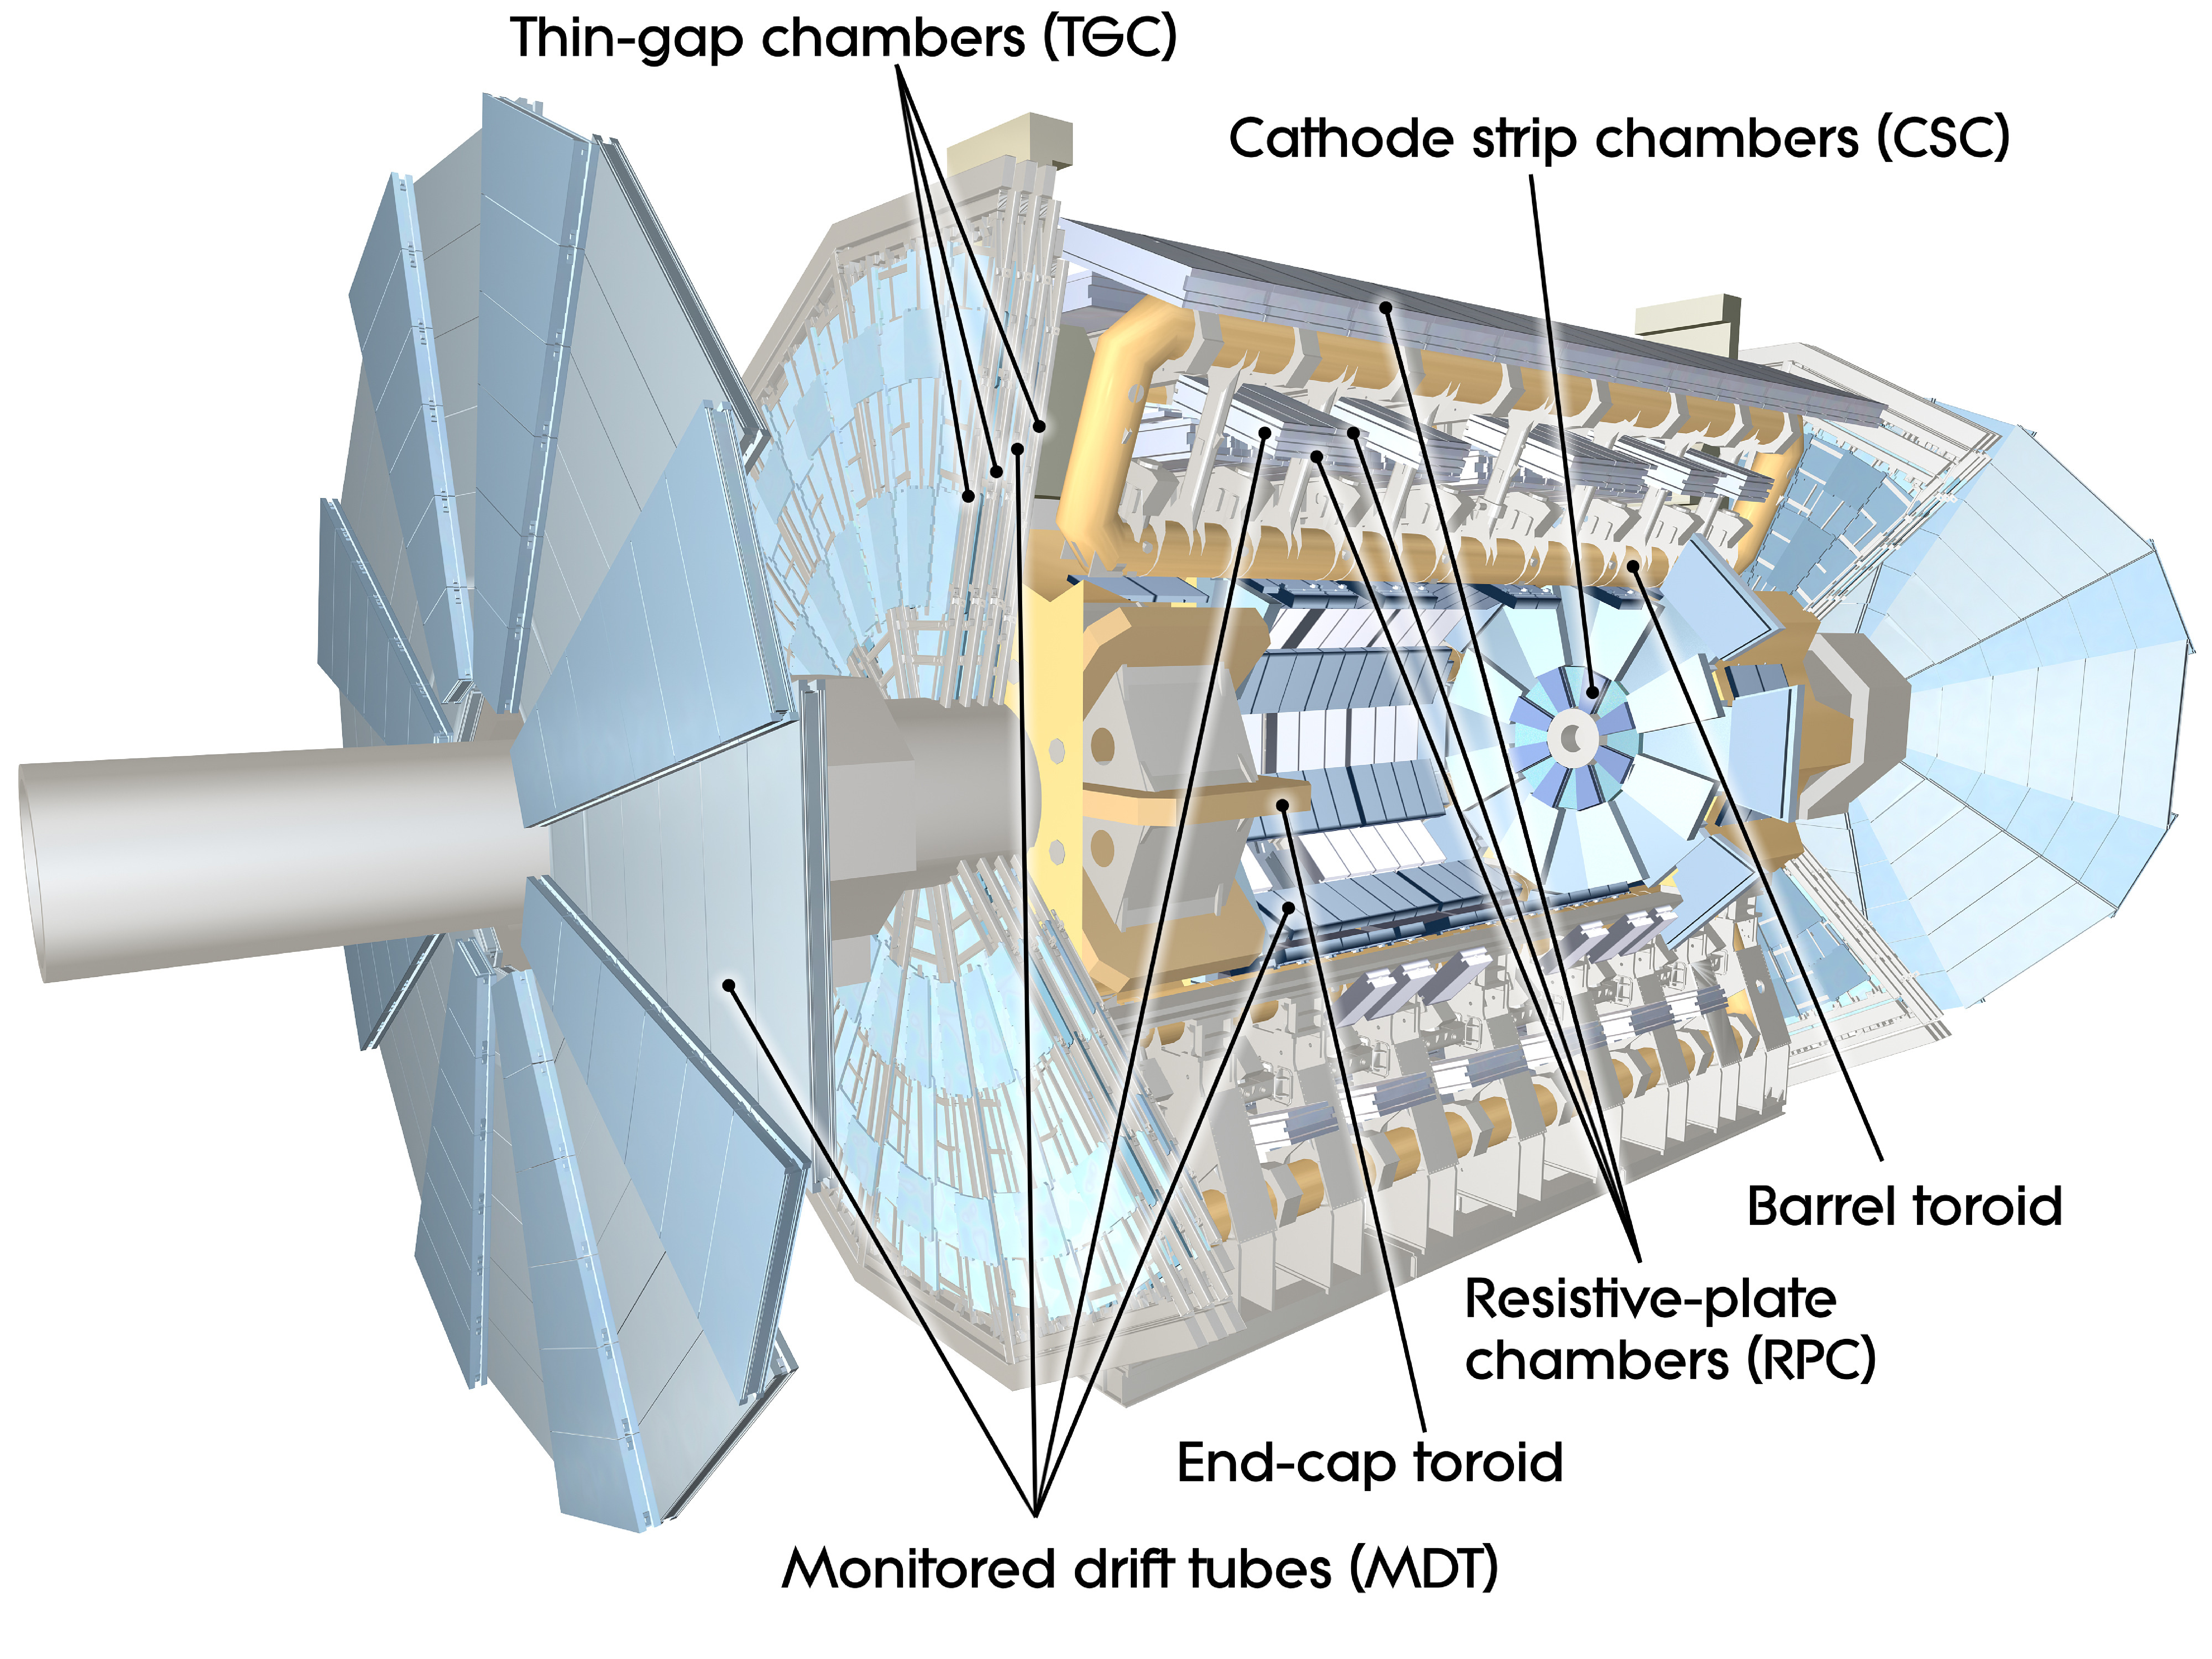
\includegraphics[width=0.60\textwidth]{muon-eps-converted-to.pdf}
\caption{Espectrómetro de muones del detector ATLAS.}
% \vspace{0.2cm}\footnotesize\textbf \sl{...}\vspace{0.2cm}
\label{muon}
\end{figure}



\section{Sistema de \textit{trigger}}

El diseño del LHC permite tener una frecuencia de cruces de haces de 40 MHz y alrededor de 23 interacciones por cruce, lo que da una tasa de interacción protón-protón del orden del GHz. Debido a que el almacenamiento y el poder de cómputo de los datos recolectados son limitados, y considerando que no todos los eventos son de interés, es necesario reducir el flujo de datos incidentes a una frecuencia de $\sim 1.5$ kHz \cite{PERF-2011-02}. El sistema de trigger, es el encargado de filtrar los eventos que son de interés, para su posterior análisis. 

El sistema de trigger de ATLAS consiste en una selección de eventos basada en dos niveles: Level 1 (L1) y el \textit{High Level Trigger} (HLT). Cada nivel permite analizar los eventos con mayor detalle, aumentando así la precisión de los criterios de selección y la complejidad de los algoritmos utilizados.

El primer nivel de trigger se encarga de la selección inicial, reduciendo la frecuencia de eventos que pasan al siguiente nivel a $\sim100$ kHz. Debido al tamaño limitado de las memorias temporales donde se guardan los datos de cada subdetector y al considerable tiempo de vuelo de las partículas hasta el espectrómetro de muones, la decisión debe tomarse en una escala de tiempo muy limitada ($2.5 \:\mu$s). El L1 está basado en hardware y selecciona objetos de alto $p_{T}$ construidos a partir de la información de varios subdetectores. Ciertas celdas del ECAL y el HCAL se utilizan entonces para enviar señales al L1 con información de los objetos. La posición de cada objeto encontrado define una <<región de interés>> (RoI) en un evento potencialmente interesante, que se extiende como un
cono desde el punto de interacción a lo largo del detector. Lo mismo en el detector de muones, que tiene diferentes cámaras que permiten obtener una estimación rápida del $p_{T}$ de los muones. El diseño del L1 le permite tener una aceptancia en el rango de $|\eta|<2.5$ para electrones, fotones, muones y taus; hasta $|\eta|<3.2$ para jets y $|\eta|<4.9$ para el cálculo de la energía transversa perdida.

\tosolve{cambiar a HLT}

El segundo nivel del trigger (L2) se centra únicamente en las RoIs donde el L1 encontró actividad, combinando información de todos los subdetectores dentro de cada una ($\sim2$ \% de la cobertura total del detector). El L2 consiste de una serie de algoritmos de reconstrucción y selección especializados, diseñados para reducir la frecuencia de eventos hasta aproximadamente 1 kHz. Estos algoritmos están implementados en \textit{clusters} de procesamiento dedicados que analizan cada evento dentro de un tiempo de latencia medio de $\sim40$ ms. El menor flujo de información en este nivel del trigger permite calcular las variables calorimétricas con mayor precisión y hacer uso de la información de las trazas reconstruidas, haciendo posible la distinción entre fotones y electrones, y el rechazo de fondo proveniente en su mayoría de jets.

La última etapa de la selección del trigger se lleva a cabo en el \textit{Event Filter}, que reduce la frecuencia de eventos a $\sim 1.5$ kHz. En este nivel se tiene acceso a toda la información del evento en los distintos subdetectores de ATLAS, con la máxima granularidad e incluyendo detalles sobre la calibración de energía de los calorímetros, la alineación de los subdetectores y el mapa de campo magnético. El tiempo de latencia relativamente largo disponible para tomar la decisión final sobre el evento ($\sim4$ s) permite la reconstrucción completa del mismo, y el refinamiento de las variables y criterios de selección al nivel de aquellos implementados en el análisis \textit{offline}. Los eventos aceptados por el EF son finalmente grabados a disco y distribuidos, accesibles \textit{offline} para todos los análisis subsecuentes.

Para cada ítem del trigger se puede asignar además un factor de escala o prescale (PS), que define la frecuencia con la que un dado ítem es evaluado por el trigger (es decir solo en uno de cada PS eventos). Se habla de una cadena de \textit{trigger unprescaled} si su factor de escala es PS = 1 en cada nivel, es decir, es evaluada en todos los eventos. La asignación de estos factores se hace incluso dinámicamente durante una toma de datos, para tener en cuenta el descenso de la luminosidad instantánea con el tiempo y mantener la tasa de procesamiento aproximadamente constante.

\section{Modelo computacional y distribución de datos}

La arquitectura computacional de ATLAS está diseñada para permitir a todos los miembros de la colaboración un acceso ágil, directo y distribuido a la gran cantidad de datos colectados por el detector ($\sim$ PB/año). La arquitectura se basa en la tecnología GRID \tosolve{cita}, compartiendo el poder de procesamiento y la capacidad de almacenamiento disponibles en distintos centros de cómputo asociados alrededor del mundo.

El software de ATLAS se desarrolla dentro un entorno C++ común llamado ATHENA \cite{ATLASComputing, Lenzi:1214931, Calafiura:865624}, en el que se realiza todo el procesamiento de datos. Los eventos aceptados por el trigger deben ser procesados para reducir su tamaño y ser utilizados para los análisis \textit{offline}. A la salida del HLT, los eventos son almacenados como \textit{Raw Data Objects} (RDOs). Luego de aplicar los algoritmos de reconstrucción y calibración, las colecciones de los distintos objetos físicos obtenidas son almacenadas en formato ESD (\textit{Event Summary Data}) y AOD (\textit{Analysis Object Data}), una versión reducida del primero ($\sim$100 kB/evento). A partir de las ESDs/AODs, se ha definido un formato de datos significativamente más pequeño (10-15 kB/evento) conocido como xAOD, sobre el que se realiza el análisis final. Las xAOD son archivos (<<ntuples>>), accesibles vía el entorno de análisis de datos ROOT \cite{Brun:1997pa}, que contienen un conjunto de variables para diferentes objetos físicos, según las necesidades de cada grupo de análisis dentro de ATLAS. 

Para agilizar el análisis final, la colaboración preselecciona eventos \textit{offline} en las llamadas derivaciones. Una de ellas, denominada EGAM1, utilizada en el presente trabajo, realiza una preselección de eventos optimizados para estudios del bosón $Z$, con una base de electrones y fotones con $p_{T} > 7 \egev$ y masa invariante de los distintos tipos de pares mayor a $50 \egev$, además de otras selecciones.

\chapter{Reconstrucción e identificación de objetos físicos}
% \addcontentsline{toc}{chapter}{Reconstrucción e identificación de objetos físicos}
\chaptermark{Reconstrucción e identificación de objetos físicos}

En el presente capítulo se describe la reconstrucción e identificación de electrones y fotones ya que son los objetos físicos principales utilizados en los estudios de esta Tesis. La reconstrucción de fotones y electrones en ATLAS se basa en las deposiciones locales de energía halladas en el ECAL, y la distinción entre unos y otros se   realiza mediante la información de las trazas reconstruidas en el ID. A su vez se aplican una serie de criterios de identificación y aislamiento, que permiten discriminarlos de falsos candidatos, o de procesos secundarios que los producen.

\section{Reconstrucción de electrones y fotones}

La  reconstrucción de fotones y electrones en ATLAS se basa en un algoritmo de clusterización \cite{Lampl:1099735} que busca deposiciones locales de energía en el calorímetro dentro de una ventana rectangular en el espacio ($\eta$, $\phi$) de tamaño fijo (\textit{Sliding Window clusterization}, SW) \cite{Monticelli:2227992}. La posición de la ventana se ajusta maximizando la energía transversa de todas las celdas contenidas. El tamaño óptimo de la ventana depende del tipo de partícula (más ancha para los electrones) a reconstruir y de la región del calorímetro (mas ancha en la región endcap). 

Aquellos \textit{clusters} electromagnéticos asociados con una traza reconstruida con $p_{T} > 0.5 \egev$, son clasificados como electrones. La definición para fotones es un poco más complicada ya que estos pueden convertir en un par $e^{+}e^{-}$ en el sector anterior al calorímetro. Los fotones convertidos están caracterizados por la presencia de al menos una traza asociada proveniente de un vértice reconstruido en el ID. La probabilidad de conversión varía entre un 40\% y un 80\% dependiendo de $\eta$, aunque solo aquellas que ocurren antes del TRT son eficientemente reconstruidas. 

Si no hay ninguna traza asociada a un dado \textit{cluster}, este es clasificado como un fotón no convertido. Aquellos \textit{clusters} asociados con trazas, que provienen de un vértice reconstruido en el ID, es clasificado como un fotón convertido. Además, para incrementar la eficiencia de reconstrucción de estos últimos, se consideran también aquellos casos donde solo una traza fue reconstruida, siempre que esta no posea ningún impacto en el B-Layer.

\section{Identificación de electrones y fotones}

La identificación de fotones se lleva a cabo mediante una serie de cortes rectangulares en un conjunto de variables que describen la forma y la estructura de las lluvias electromagnéticas según se propagan en el detector. Estas variables incluyen información de los calorímetros y, para el caso de fotones convertidos, del detector de trazas. Se definen dos conjuntos de cortes dependiendo de la rigurosidad de los mismos: \textit{loose} y \textit{tight}. Los cortes de cada conjunto han sido optimizados para asegurar una alta eficiencia de identificación de electrones/fotones aislados y de rechazo de fondo. 

Para la identificación de electrones se utiliza un algoritmo de identificación basado en el método de \textit{likelihood} (LH). El mismo consiste en una técnica de análisis multivariable que evalúa simultáneamente distintas propiedades de los candidatos a la hora de realizar la selección. El LH utiliza las funciones de densidad de probabilidad (PDFs) de la señal y del fondo de las distintas variables que describen a la lluvia electromagnética. Basada en esas PDFs, se calcula una probabilidad total del objeto de ser señal o fondo. Adicionalmente se utilizan variables discriminantes que se basan en la cantidad de impactos en el detector de trazas. Se utilizan tres cortes de discriminación: \textit{loose}, \textit{medium} y \textit{tight}. Los mismos se definen de tal forma de que los objetos seleccionado por uno sean un subconjunto de los otros. Es decir, los seleccionados por \textit{medium} son seleccionados también por \textit{loose}, y los seleccionados por \textit{tight} son seleccionados también por \textit{medium}.


La definición de algunas variables que determinan los distintos cortes se detallan a continuación. La definición de los cortes se muestra en la Tabla \ref{lmttable}.


\begin{itemize}

	\item \textbf{Fuga hadrónica}

		Es la energía transversa depositada en el calorímetro hadrónico, normalizada a la energía transversa del cluster electromagnético.

		\begin{equation}
		R_{\text{had}_{(1)}}=\frac{E_{T}^{\text{had}}}{E_{T}}
		\end{equation}

		En la región de transición barrel-endcap del HCAL, se utiliza el depósito de energía en todo el calorímetro hadrónico para minimizar los efectos de la degradación de resolución ($R_{\text{had}}$). En el resto del detector, se mide sólo la energía hadrónica depositada en la primera capa del HCAL ($R_{\text{had}_{(1)}}$).

	\item  \textbf{Perfil lateral de energía en $\eta$ (2$^{\text{da}}$ capa del ECAL)}

		\begin{equation}
		R_{\eta}=\frac{E_{3\times 7}^{S2}}{E_{7\times 7}^{S2}}
		\end{equation}

 		donde $E_{i\times j}^{S2}$ es la suma de las celdas en la segunda capa del calorímetro electromagnético contenidas en una ventana $i\times j$ (en $\Delta \eta \times \Delta \phi$).

	\item  \textbf{Perfil lateral de energía en $\phi$ (2$^{\text{da}}$ capa del ECAL)}

		\begin{equation}
		R_{\phi}=\frac{E_{3\times 3}^{S2}}{E_{3\times 7}^{S2}}
		\end{equation}

 		donde $E_{i\times j}^{S2}$ es la suma de las celdas en la segunda capa del calorímetro electromagnético contenidas en una ventana $i\times j$ (en $\Delta \eta \times \Delta \phi$).

	\item  \textbf{RMS del perfil lateral de energía en $\eta$ (2$^{\text{da}}$ capa del ECAL)}


		\begin{equation}
		w_{\eta_{2}}=\sqrt{\frac{\sum E_{i}\eta_{i}^{2}}{\sum E_{i}}- \left(\frac{\sum E_{i}\eta_{i}}{\sum E_{i}}\right)^{2}}
		\end{equation}

		mide el ancho lateral de las lluvias electromagnéticas, donde $E_{i}$ es la energía de la i-ésima celda del calorímetro electromagnético contenida en una ventana de $3\times 5$ celdas en $\eta \times \phi$.

	\item  \textbf{Perfil lateral de energía en $\eta$ (1$^{\text{ra}}$ capa del ECAL)}

		\begin{equation}
		F_{\text{side}}=\frac{E(\pm 3)-E(\pm 1)}{E(\pm 1)}
		\end{equation}

		mide la contención lateral de la cascada electromagnética a lo largo de $\eta$. $E(\pm n)$ es la energía en las $\pm n$ celdas alrededor de aquella con la deposición máxima.

	\item  \textbf{RMS del perfil lateral de energía en $\eta$ (3 \textit{strips}, 1$^{\text{ra}}$ capa del ECAL)}

		\begin{equation}
		w_{s,3}=\sqrt{\frac{\sum E_{i}(i-i_{\text{max}})^{2}}{\sum E_{i}}}
		\end{equation}

		mide el ancho de la lluvia electromagnética a lo largo de $\eta$ en la primera capa del calorímetro electromagnético usando solo la banda con mayor deposición de energía ($i_{\text{max}}$) y sus vecinas inmediatas.

	\item  \textbf{RMS del perfil lateral de energía en $\eta$ (total, 1$^{\text{ra}}$ capa del ECAL)}

		$w_{s,\text{tot}}$ está definida de la misma forma que $w_{s,3}$, pero utiliza todas las bandas de la primera capa del calorímetro electromagnético en una ventana $\Delta\eta\times\Delta\phi = 0.0625 \times 0.2$, que corresponde aproximadamente a $20\times 2$ bandas en $\eta \times \phi$.

	\item  \textbf{Diferencia al segundo máximo}

		\begin{equation}
		\Delta E=[E_{2^{nd} \:\text{max}}^{S1} - E_{\text{min}}^{S1}]
		\end{equation}

		es la diferencia entre la energía de la banda con la segunda energía más grande $E_{2^{nd} \:\text{max}}^{S1}$ , y la mínima energía $E_{\text{min}}^{S1}$ entre la anterior y la celda con la máxima deposición. En caso de no haber segundo máximo se fija $\Delta E = 0$.

	\item  \textbf{Asimetría de los dos máximos locales en $\eta$}

		\begin{equation}
		\Delta E_{\text{ratio}}=\frac{E_{1^{st} \:\text{max}}^{S1} - E_{2^{nd} \:\text{max}}^{S1}}{E_{1^{st} \:\text{max}}^{S1} + E_{2^{nd} \:\text{max}}^{S1}}
		\end{equation}
 
 		mide la diferencia relativa entre las energías de las dos celdas con máxima deposición. En caso de no haber segundo máximo se fija $E_{\text{ratio}} = 1$.


\end{itemize}

\renewcommand{\arraystretch}{1.0}
\begin{table}	
\centering
\caption{Detalle de las diferentes variables usadas para la selección \textit{loose} (L) y \textit{tight} (T) de fotones y electrones. El $\checkmark$ indica cuándo la selección requiere de esa variable\cite{ATLAS:2016iqc} \cite{Tripiana:1433788}.}
 \makebox[0.5\textwidth][c]{
 \begin{tabular}{ r p{8cm} c | c c | c }

	\hline

	\multirow{2}{*}{Categoría} & \multirow{2}{*}{Descripción} & \multirow{2}{*}{Nombre} & \multicolumn{2}{ c |}{$\gamma$} & \multirow{2}{*}{$e$} \\

		&	&	& L & T &   \\

	\hline

	Aceptancia & $|\eta| < 2.37$, excluyendo $1.37 < |\eta| < 1.52$  & - & $\times$ & $\checkmark$ & $\times$  \\

	Fuga hadrónica & Cociente entre $E_{T}$ en la primera capa del calorímetro hadrónico y $E_{T}$ del \textit{cluster} electromagnético & $R_{\text{had}_{1}}$ & $\checkmark$ & $\checkmark$ & $\checkmark$ \\

		& Cociente entre $E_{T}$ en todo el calorímetro hadrónico y $E_{T}$ del \textit{cluster} electromagnético $(|\eta| \le 0.8$ y $|\eta| \ge 1.37)$ & $R_{\text{had}}$ & $\checkmark$ & $\checkmark$ & $\checkmark$  \\

	ECAL (3$^{ra}$ capa) & Fracción de energía en la tercer capa del ECAL & $f_{3}$ & $\times$ & $\times$ & $\checkmark$  \\
	

	ECAL (2$^{da}$ capa) & Ancho lateral de la lluvia en dirección de $\eta$ & $w_{\eta_{2}}$ & $\checkmark$ & $\checkmark$ & $\checkmark$ \\

		& Cociente entre la suma de las energías de las 3 $\times$ 7 celdas y la suma de 5 $\times$ 7 celdas, ambas en torno al centro del \textit{cluster} & $R_{\eta}$ & $\checkmark$ & $\checkmark$ & $\checkmark$ \\

		& Cociente entre la suma de las energías de las 3 $\times$ 3 celdas y la suma de 3 $\times$ 7 celdas, ambas en torno al centro del \textit{cluster} & $R_{\phi}$ & $\times$ & $\checkmark$ & $\checkmark$ \\

	ECAL (1$^{ra}$ capa) & Ancho lateral de la lluvia en 3 \textit{strips} alrededor del máximo & $w_{s,3}$ & $\times$ & $\checkmark$ & $\times$ \\

		& Ancho lateral total de la lluvia & $w_{s,\text{tot}}$ & $\times$ & $\checkmark$ & $\checkmark$ \\

		& Fracción de energía fuera de las 3 \textit{strips} centrales pero dentro de las 7 & $F_{\text{side}}$ & $\times$ & $\checkmark$ & $\times$ \\

		& Diferencia entre la energía de la \textit{strip} con el segundo mayor depósito y la menor energía entre los dos primeros máximos locales & $\Delta E$ & $\times$ & $\checkmark$ & $\times$ \\

		& Asimetría entre el primer y segundo máximo & $E_{\text{ratio}}$ & $\times$ & $\checkmark$ & $\checkmark$  \\

		& Fracción de energía en la primera capa del ECAL & $f_{1}$ & $\times$ & $\times$ & $\checkmark$  \\

	ID & Parámetro de impacto transverso& $d_{0}$ & $\times$ & $\times$ & $\checkmark$ \\

		& Momento perdido en la traza entre el primer punto de detección y el último, dividido el momento total original & $\Delta p/p$ & $\times$ & $\times$ & $\checkmark$  \\

	TRT & Probabilidad \textit{likelihood} basa en la radiación de transición en el TRT & eProbabilityHT & $\times$ & $\times$ & $\checkmark$  \\

	ECAL+ID & $\Delta\eta$ entre la traza extrapolada al calorímetro y el \textit{cluster} en la primer capa& $\Delta\eta_{1}$ & $\times$ & $\times$ & $\checkmark$ \\

	\hline

\end{tabular}}
\label{lmttable}
\end{table}
\renewcommand{\arraystretch}{1}

Por último un algoritmo adicional es aplicado para resolver ambigüedades residuales en candidatos a fotones que son también reconstruidos como electrones. Diferentes estrategias son utilizadas dependiendo del estado de conversión de los fotones según es explica en la Referencia \cite{ambiguity}.


\section{Criterios de aislamiento}

Luego de realizar la identificación, es necesario distinguir entre electrones y fotones directos (aquellos producidos en la colisión), mal reconstruidos o de los no directos producidos de decaimientos de hadrones ($\pi^{0}$, $\eta$, etc.) dentro de jets.

Los fotones o electrones provenientes por ejemplo, del punto de interacción, o los electrones provenientes de $Z\rightarrow ee$, poseen baja actividad hadrónica en su vecindad. En cambio en los no directos, se espera que haya un gran actividad provenientes de los objetos que acompañan al jet dentro del que fueron producidos o erróneamente identificados. Para realizar esta distinción se utiliza un criterio de aislamiento que se basa en medidas calorimétricas o en las trazas reconstruidas en el entorno del objeto.

El aislamiento de trazas se define a partir de considerar un cono de radio $R=\sqrt{\Delta\eta^{2}+\Delta\phi^{2}}$ centrado en el baricentro del \textit{cluster} electromagnético asociado al objeto. A todas las trazas dentro de este cono se le pueden aplicar ciertos cortes, como $p_{T}>1 \egev$, impactos en el SCT, etc. Además, se requiere que aquellas trazas en un cono interno con $R=0.1$, no provengan de un vértice de conversión, a fin de remover los fotones convertidos. El aislamiento de trazas ha mostrado ser altamente eficiente tanto para retener señal como para rechazar falsos candidatos del fondo, aún luego de la selección descripta en la sección anterior. Aun así, el criterio más utilizado es el aislamiento calorimétrico.

El aislamiento calorimétrico, $E_{T}^{\text{iso}}$, es calculado a partir de las celdas en ambos calorímetros (ECAL y HCAL). Nuevamente se define un cono con un cierto radio $R$ centrado en el baricentro del \textit{cluster} del objeto, y la suma de la energías de todas las celdas contenidas en ese cono se denomina $E_{T}^{\text{iso}}$. 

A fin de remover la contribución energética de la lluvia electromagnética desarrollada por el propio objeto al cono de aislamiento, el núcleo central de $N_{\eta}\times N_{\phi} = 5 \times 7$ celdas en el segundo compartimiento del ECAL, es ignorado en la suma, como se esquematiza en la Figura \ref{isolation}. Se considera que dentro de esta región ignorada, se concentra el 95\% de la energía de la lluvia electromagnética, por lo que solo el 5\% de la energía del objeto contribuye a esta región. Por otro lado, todas las celdas contenidas dentro del cono en el HCAL son consideradas para la suma, ya que se espera que el ECAL contenga toda lluvia electromagnética desencadenada por el objeto inicial. 

Para fotones, el valor típico de $R$ es $0.4$, y el corte de aislamiento es $E_{T}^{\text{iso}}<2.45 \egev + 0.022 \times p_{T}$ (donde el $p_{T}$ corresponde al momento transverso del objeto reconstruido e identificado). En cambio los electrones pasan por un criterio que tiene dependencia en $\eta$ y $p_{T}$ denominado \textit{Gradient Loose}, con requerimientos tanto en las variables calorimétricas como en las asociadas a la traza \cite{ATL-PHYS-PUB-2015-037_extra}.


% En cambio en los electrones pasan por un criterio denominando \textit{Gradient Loose}, en el cual el valor de $R$ depende del $p_{T}$ de los mismos. En este caso para el aislamiento calorimétrico $R=0.2$ y para el aislamiento de trazas $R=10\egev/p_{T}$

\begin{figure}
\centering
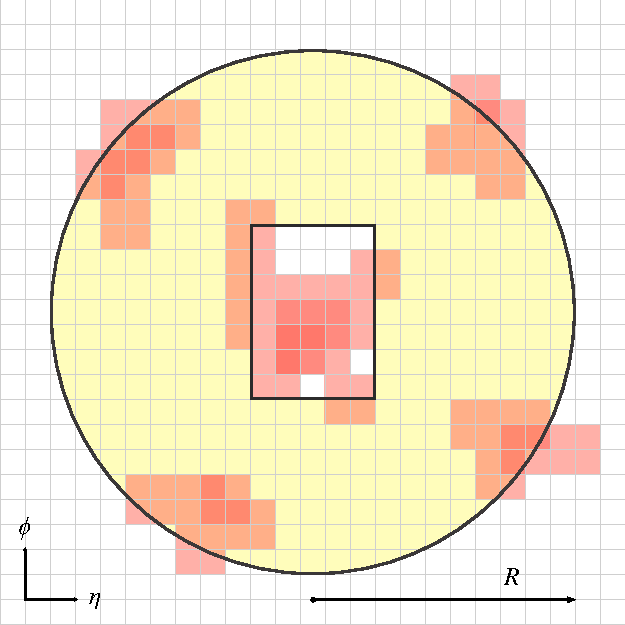
\includegraphics[width=0.50\textwidth]{iso.pdf}
\caption{Esquema ilustrando el cálculo de la energía de aislamiento del fotón. La \textit{grid} representa la granularidad de las celdas del calorímetro electromagnético. El cono de color amarillo de radio $R$ rodea al candidato. La energía del candidato a fotón o electrón está mayormente contenida en el rectángulo central de $5 \times 7$ en $\Delta\eta \times \Delta\phi$.}
\label{isolation}
\end{figure}

\section{Energía faltante}

Una variable de suma importancia en la búsqueda de partículas supersimétricas, es la energía transversa faltante ($\met$). Como se mencionó anteriormente, el momento transverso se debe conservar en todo el proceso, y cualquier desequilibrio en el mismo se lo asocia a $\met$. Puede indicar la presencia de partículas indetectables como neutrinos o nuevas partículas estables, o que interactúan débilmente con la materia.

El momento transverso faltante ($p_{T}^{\text{miss}}$) se define como el valor negativo de la suma del momento transverso de todas las partículas detectadas, y su magnitud es lo que se denomina energía transversa faltante. Esta es calculada con un algoritmo basado en objetos \cite{Khoo:2012749}. El algoritmo utiliza los objetos físicos construidos y calibrados descriptos en las secciones anteriores. Los depósitos de energía en el calorímetro (topo-clusters) son asociados a los objetos de alto $p_{T}$ en el siguiente orden: electrones, fotones, jets y muones. Los depósitos que no están asociados a ningún objeto son incluidos en el término \textit{soft}. El momento transverso es calculado entonces como:

\begin{equation}
p_{T}^{\text{miss}}=\left(p_{T}^{\text{miss}}\right)^{e} + \left(p_{T}^{\text{miss}}\right)^{\gamma} + \left(p_{T}^{\text{miss}}\right)^{\text{jet}} +\left(p_{T}^{\text{miss}}\right)^{\mu} + \left(p_{T}^{\text{miss}}\right)^{\text{soft}}
\end{equation}

\noindent
donde cada término es calculado como el negativo de la suma de los objetos reconstruidos y calibrados, más el término \textit{soft}. La contribución de los taus, se incluye en el término de jets o en el \textit{soft}, debido a que los mismos decaen hadrónicamente. Finalmente la energía transversa faltante se define como:

\begin{equation}
\met=|p_{T}^{\text{miss}}|
\end{equation}



\clearpage

\chapter{Estrategia general de análisis de datos para búsqueda de nueva física}
% \addcontentsline{toc}{chapter}{Estrategia general del análisis}
\chaptermark{Estrategia general de análisis de datos para búsqueda de nueva física}



El análisis para el cual está orientada esta Tesis consiste en la búsqueda de Supersimetría en eventos con un fotón aislado muy energético, jets y gran cantidad de energía faltante en estado final \cite{Alonso:2147473,ATLAS:2016fks,Collaboration:2198651}. La estrategia general de la búsqueda consiste en el conteo del número de eventos observado en exceso sobre el SM en una cierta región del espacio de observables rica en eventos de la señal considerada.


\section{Identificación de eventos de fondo}

Para un correcto procedimiento, es necesario conocer los procesos del SM que tengan un estado final equivalente a de la señal buscada. Estos eventos toman el rol de fondo en el contexto de un análisis de búsqueda de SUSY. Para este análisis, son procesos que tienen un fotón, jets y energía faltante en el estado final, y pueden dividirse en varias categorías. Por un lado, los procesos que dan lugar a eventos con un fotón y energía faltante real, es decir, los que se llaman fondos irreducibles. Estos son:

\begin{itemize}

	\item $Z(\rightarrow \nu\nu)$ + $\gamma$

	\item $W (\rightarrow l\nu)$ + $\gamma$

	\item $t \overline{t}$ + $\gamma$

\end{itemize}

También es posible que, aunque el proceso no tenga fotones en el estado final, un electrón o un jet sean identificados como un fotón, dando lugar a un estado final idéntico al buscado. En esta categoría están:

\begin{itemize}

	\item $W (\rightarrow l\nu)$ + jets

	\item $Z (\rightarrow \nu\nu)$ + jets

	\item $t \overline{t}$

	\item $WW$, $ZZ$, $WZ$

\end{itemize}

Y por último, también puede haber procesos que a pesar de no generar energía faltante real, poseen lo que se denomina energía faltante instrumental, proveniente generalmente de la incorrecta reconstrucción de la energía de los jets. De esta manera, pueden dar lugar a eventos con el estado final de interés, los procesos QCD:

\begin{itemize}

	\item $\gamma$ + jets

	\item multijet, con alguno de los jets identificado como fotón

	\item $Z(\rightarrow ll)$ + jets, donde un leptón o un jet es identificado como un fotón

\end{itemize}



\section{Regiones de señal, control y validación}

Al estudiar fenómenos de nueva física es necesario definir una región en el espacio de observables, donde el modelo de señal predice un exceso significativo de eventos sobre el nivel de fondo. Esta región se llama región de señal (SR). El análisis de búsqueda consiste básicamente en estimar entonces las contribuciones de los procesos del SM que contaminan esta región. Para esto existen dos técnicas principales: utilizar directamente simulaciones Monte Carlo, o utilizar métodos basados en los propios datos observados. En algunos casos se emplea un tercer método para estimar los fondos, que consiste en utilizar la estimación proveniente de las simulaciones MC, pero corregida a partir de los datos. Para esto se definen regiones de control (CR) en las cuales el fondo dominante pueda ser comparado y normalizado con los datos observados en esa misma región. 

Otra componente importante del análisis es la validación de los métodos utilizados para predecir los fondos. Con este objetivo se definen regiones de validación (VR) que se encuentren entre las CR y las SR en términos de los principales observables cinemáticos en los criterios de selección. El diseño de las VRs comprende un compromiso entre minimizar la contaminación de la señal, y a su vez ser efectivas en la validación de la extrapolación entre CR y SR. Es importante que las CR, VRs y SRs sean estadísticamente independientes para poder combinar la PDF que modela cada región en una PDF conjunta. En la Figura \ref{regions} se puede ver como ejemplo, un esquema de las regiones descriptas anteriormente.

Durante todo el análisis se utiliza una estrategia denominada <<blinding>>. La misma consiste en realizar el análisis predictivo del eventos del SM sin mirar la cantidad de eventos de datos en la SR. De esta forma se evita un sesgo en la elección de las SR y por ende en la cantidad de eventos finales.

\begin{figure}
\centering
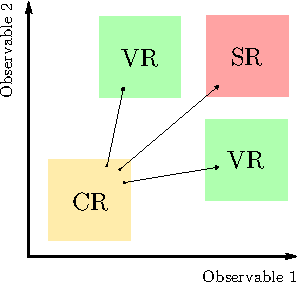
\includegraphics[width=0.40\textwidth]{regions.pdf}
\caption{Esquema del diseño de las regiones de señal (SR), control (CR) y validación (VR) en términos de dos observables arbitrarios.}
\label{regions}
\end{figure}

\section{Selección de eventos}

El análisis para el cual está orientada esta Tesis \cite{Collaboration:2198651} se basa en la utilización de dos regiones de señal que son comparadas con las predicciones del SM. La primera de las regiones (SR$_{\text{L}}$), está optimizada para gluinos muy masivos y neutralinos con baja masa o intermedia. Se caracteriza por una alta multiplicidad de jets y actividad hadrónica, y baja energía faltante. La segunda región (SR$_{\text{H}}$) está orientada a escenarios donde la masa del gluino y el neutralino son más cercanas. Esto produce una baja multiplicidad de jets y actividad hadrónica, una producción de fotones de alto $p_{T}$ y una alta energía transversa faltante.

Para definir los observables a ser utilizados en la construcción las distintas regiones es importante tener en cuenta que en partículas supersimétricas muy masivas, es de esperar una elevada energía transversa total ($H_{T}$), definiendo a $H_{T}$ como:

\begin{equation}
H_{T}=|p_{T}^{\gamma}|+\sum_{\text{jets}}|p_{T}^{\text{jet}}|
\end{equation} 

\noindent
que es definitiva la suma escalar del momento transverso de todos los jets más la del fotón \textit{leading}. Para la selección de eventos de señal se utiliza una variable, $m_{\text{eff}}$, que es la suma escalar de $H_{T}$ y $\met$, que tiene en cuenta ambas características del estado final. En ambas regiones se solicita que no se produzcan leptones y que se produzca al menos un fotón. Además, en la SR$_{\text{L}}$ más de 4 jets son requeridos, mientras que en la SR$_{\text{H}}$ más de dos.

En los eventos caracterizados por una elevada $\met$, el vector de energía transversa faltante tiende a estar alineado con el fotón o con alguno de los dos \textit{leading} jets. Para suprimir este fondo se utiliza una selección basada en la separación angular de estos objetos, $\Delta\phi$(jet, $\met$) y $\Delta\phi$($\gamma$, $\met$), para eventos con $\gamma/W$ + jets.

Finalmente se define una variable, $R_{T}^{4}$, definida como:

\begin{equation}
R_{T}^{4}=\frac{\sum_{i}^{4}p_{T}^{i}}{\sum_{j}p_{T}^{j}}
\end{equation}

\noindent
donde el numerador es una suma sobre los 4 jets con $p_{T}$ más alto, y el denominador es una suma sobre todos los jets \cite{Collaboration:2198651}. Las señales de SUSY consideradas en este análisis se caracterizan por tener varios jets con alto $p_{T}$, produciendo valores de $R_{T}^{4}$ menores a 1. Contrariamente, los fondos del SM no comparten esta característica, por lo que los valores de $R_{T}^{4}$ son cercanos a 1.

Los criterios de selección para ambas regiones de señal se resumen en la Tabla \ref{srs}.

\begin{table}
\centering
\caption{Criterios de selección para las SR$_{\text{L}}$ y SR$_{\text{H}}$ \cite{ATLAS:2016fks}.}
\begin{tabular}{ l | r | r }

	\hline

	& SR$_{\text{L}}$ & SR$_{\text{H}}$ \\

	\hline

	$N_{\text{fotones}}$ 	& $> 0$ 	& $> 0$ \\

	$N_{\text{leptones}}$ 	& $=0$ 	& $=0$ \\

	$N_{\text{jets}}$ 	& $>4$ 	& $>2$ \\

	$p_{T}^{\text{leading}\: \gamma}$ 	& $> 145 \egev$ 	& $> 400 \egev$ \\

	$\Delta\phi(\text{jet},\: E_{T}^{\text{miss}})$ 	& $> 0.4$ 	& $> 0.4$ \\

	$\Delta\phi(\gamma$,\: $E_{T}^{\text{miss}})$ 	& $>0.4$ 	& $>0.4$ \\

	$\met$ 	& $>200\egev$ 	& $>400\egev$ \\

	$m_{\text{eff}}$ 	& $> 2000 \egev$ 	& $> 2000 \egev$ \\

	$R_{T}^{4}$ 	& $< 0.9$ 	& - \\

	\hline


\end{tabular}
\label{srs}
\end{table}

Una vez definidas las regiones de señal se definen tres regiones de control, denominadas CRW, CRT y CRQ, utilizadas para la normalización de eventos de $W\gamma$, $\ttbar\gamma$ y QCD $\gamma + \text{jets}$, respectivamente. Las mismas variables que definen las SR son empleadas para establecer las CRs. Se agregan además otros requisitos para disminuir la contaminación o aumentar el número de eventos de un cierto proceso; como por ejemplo colocar un máximo para la $E_{T}^{\text{miss}}$ o requerir la producción de b-jets. La Tabla \ref{crs} muestra las selecciones utilizadas para definir las CRs.

\begin{table}
\centering
\caption{Criterios de selección para las CRs basadas en las SRs. Los valores de CRW y CRT son los mismos para ambas regiones de señal.}
\makebox[0.5\textwidth][c]{
\begin{tabular}{ l | r r r | r r r }

	\hline

	& \multicolumn{3}{c |}{SR$_{\text{L}}$} & \multicolumn{3}{c}{SR$_{\text{H}}$} \\

	\hline

	 & CRQ & CRW & CRT & CRQ & CRW & CRT \\

	 \hline

	$N_{\text{fotones}}$ 	& $=1$ & $>0$ & $>0$ & $=1$ & $>0$ & $>0$ \\

	$N_{\text{leptones}}$ 	& $=0$ & $>0$ & $>0$ & $=0$ & $>0$ & $>0$ \\

	$N_{\text{jets}}>$ 		& $4$ &	-	& $1$ & $2$ &	-	& $1$ \\

	$N_{\text{b-jets}}$ 	& - &	$=0$	& $>1$ & - &	$=0$	& $>1$\\

	$p_{T}^{\text{leading}\: \gamma} [\egev]>$ 	& $145$ 	& $145$ 	& 	$145$ & $400$ 	& $145$ 	& 	$145$\\

	$\Delta\phi(\text{jet},\: E_{T}^{\text{miss}})>$ 	& $0.4$ 	& $0.4$ 	&  $0.4$& $0.4$ 	& $0.4$ 	&  $0.4$\\

	$\Delta\phi(\gamma$,\: $E_{T}^{\text{miss}})>$	& $0.4$ 	& - 	& -	& $0.4$ 	& - 	& -\\

	$\met [\egev]$ & $<50$ & $[100-200]$ & $[50-200]$ & $<50$ & $[100-200]$ & $[50-200]$ \\

	$m_{\text{eff}} [\egev]>$ 	& $1500$ 	& $500$ 	& $500$	& $2000$ 	& $500$ 	& $500$\\

	$R_{T}^{4}$ 	& $<0.9$ 	& - 	& -	& - 	& - 	& -\\

	\hline

\end{tabular}}
\label{crs}
\end{table}


Junto con estas regiones se utilizan las ya mencionadas regiones de validación, para verificar la estimación del fondo. Estas fueron diseñadas para ser similares a las SRs, pero con alguno de los criterios modificado o invertido, y de esta forma evitar que se contaminen con señal. La región de validación denominada VRL está diseñada para enriquecer los fondos provenientes de $W\gamma$ y $\ttbar\gamma$, mientras que las VRM y VRD son utilizadas para validar la extrapolación del fondo de $\gamma$ + jets de la CR a la SR. Así por ejemplo, la VRM1 (asociada a SR$_{\text{H}}$) está definida con $m_{\text{eff}}>1000\egev$ y $125\egev<\met<175\egev$, mientras que la VRM2 (asociada a SR$_{\text{L}}$) se define con $m_{\text{eff}}>1500\egev$ y $75\egev<\met<175\egev$. Por otro lado, y como otro ejemplo, la VRL1 está definida con los mismos requisitos que la SR pero requiriendo al menos un leptón, $\met<200\egev$ y $m_{\text{eff}}>1000\egev$ \cite{ATLAS:2016fks}.




% Por ejemplo, una VR asociada a SR$_{H}$ se define con $m_{\text{eff}}>1000 \egev$ y con $125 \egev < E_{T}^{\text{miss}} < 175 \egev$. \tosolve{citar las de ICHEP}


La Figura \ref{SRL_SRH} muestra un resumen de los resultados obtenidos en todas las regiones de control, validación y señal, como fueron obtenidas en el análisis de la Referencia \cite{ATLAS:2016fks}. Se encuentra un buen acuerdo entre los datos y los fondos del SM predichos en las VRs, y no se observa un exceso significativo en las SRs. Los números de eventos obtenidos de las distintas contribuciones de fondos para ambas regiones de señal se observan en la Tabla \ref{ta:SRL_SRH}. 

\begin{figure}

	\begin{subfigure}{0.5\textwidth}
		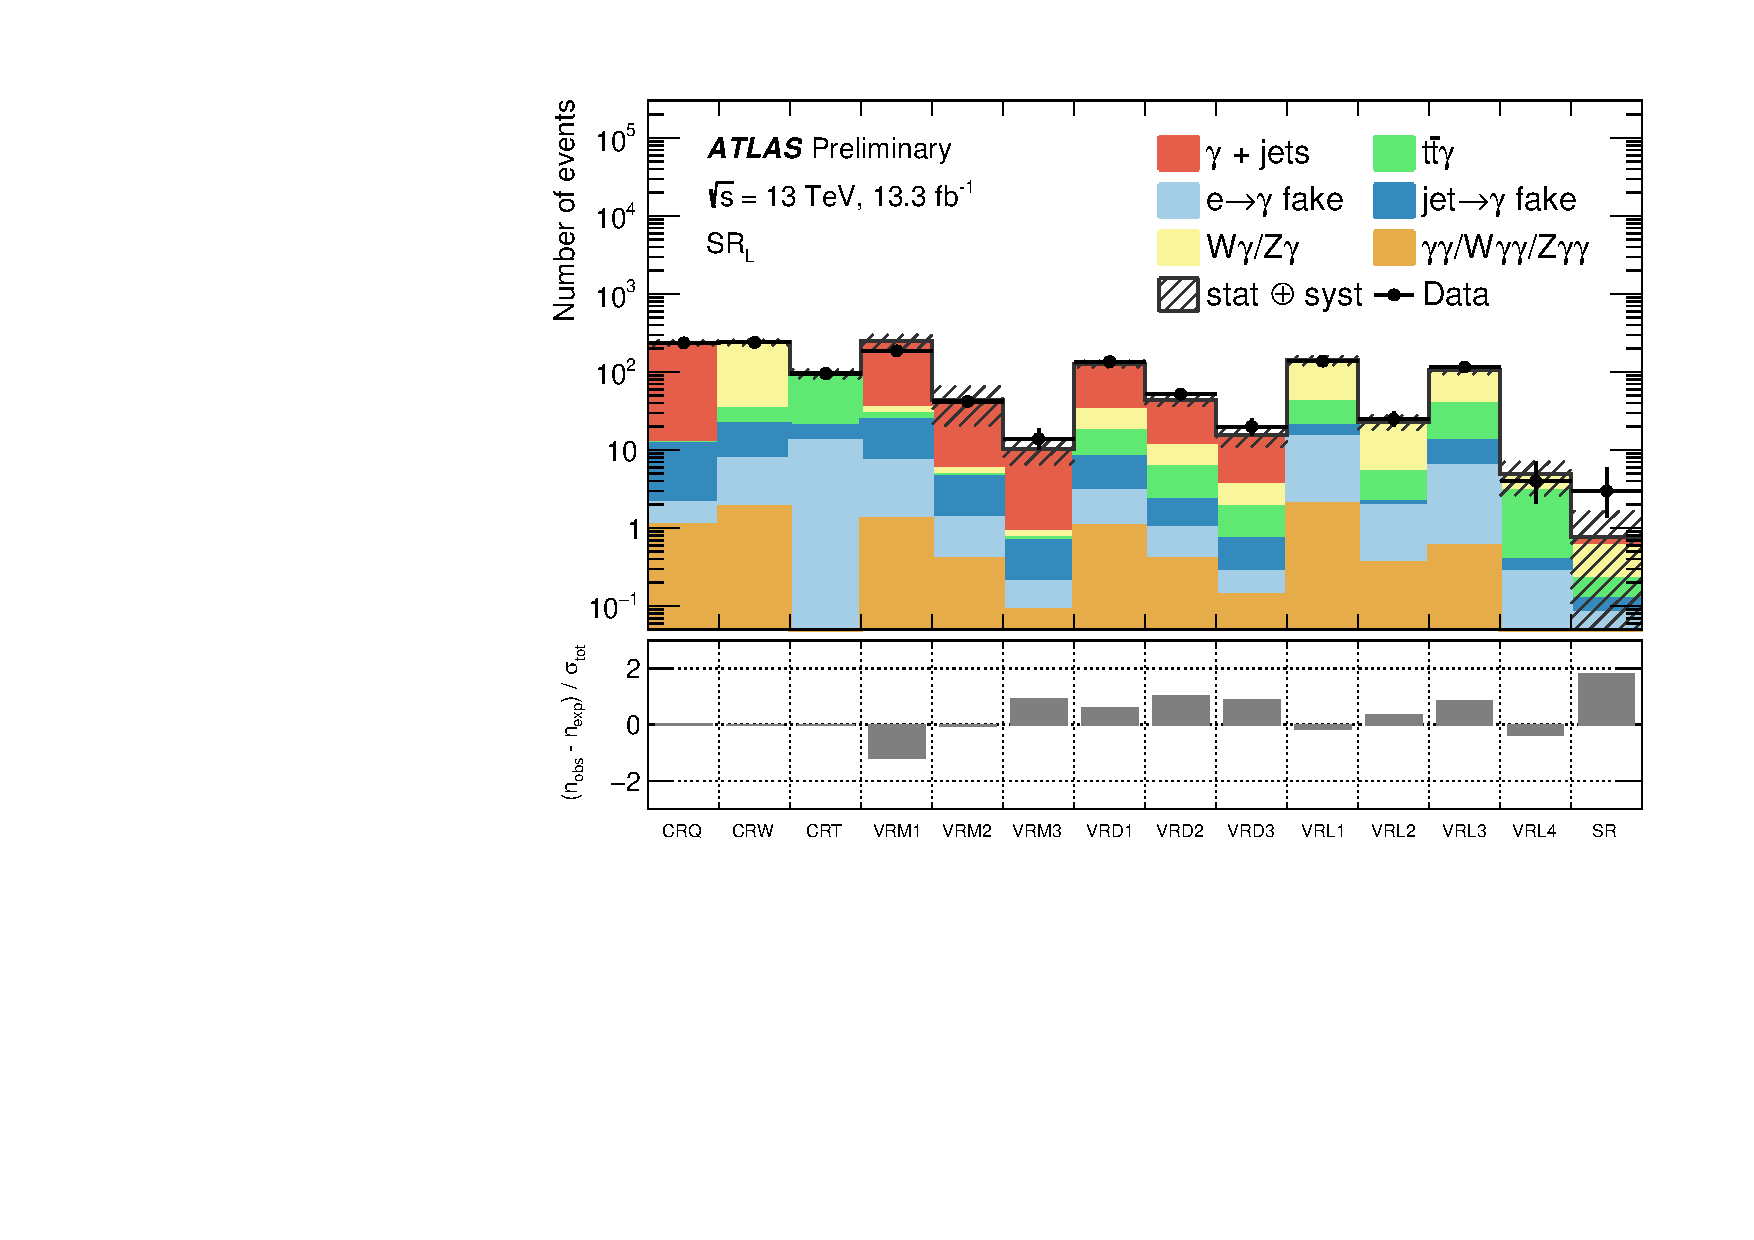
\includegraphics[scale=0.40]{SRL.pdf} 
	\end{subfigure}
	~
	\begin{subfigure}{0.5\textwidth}
		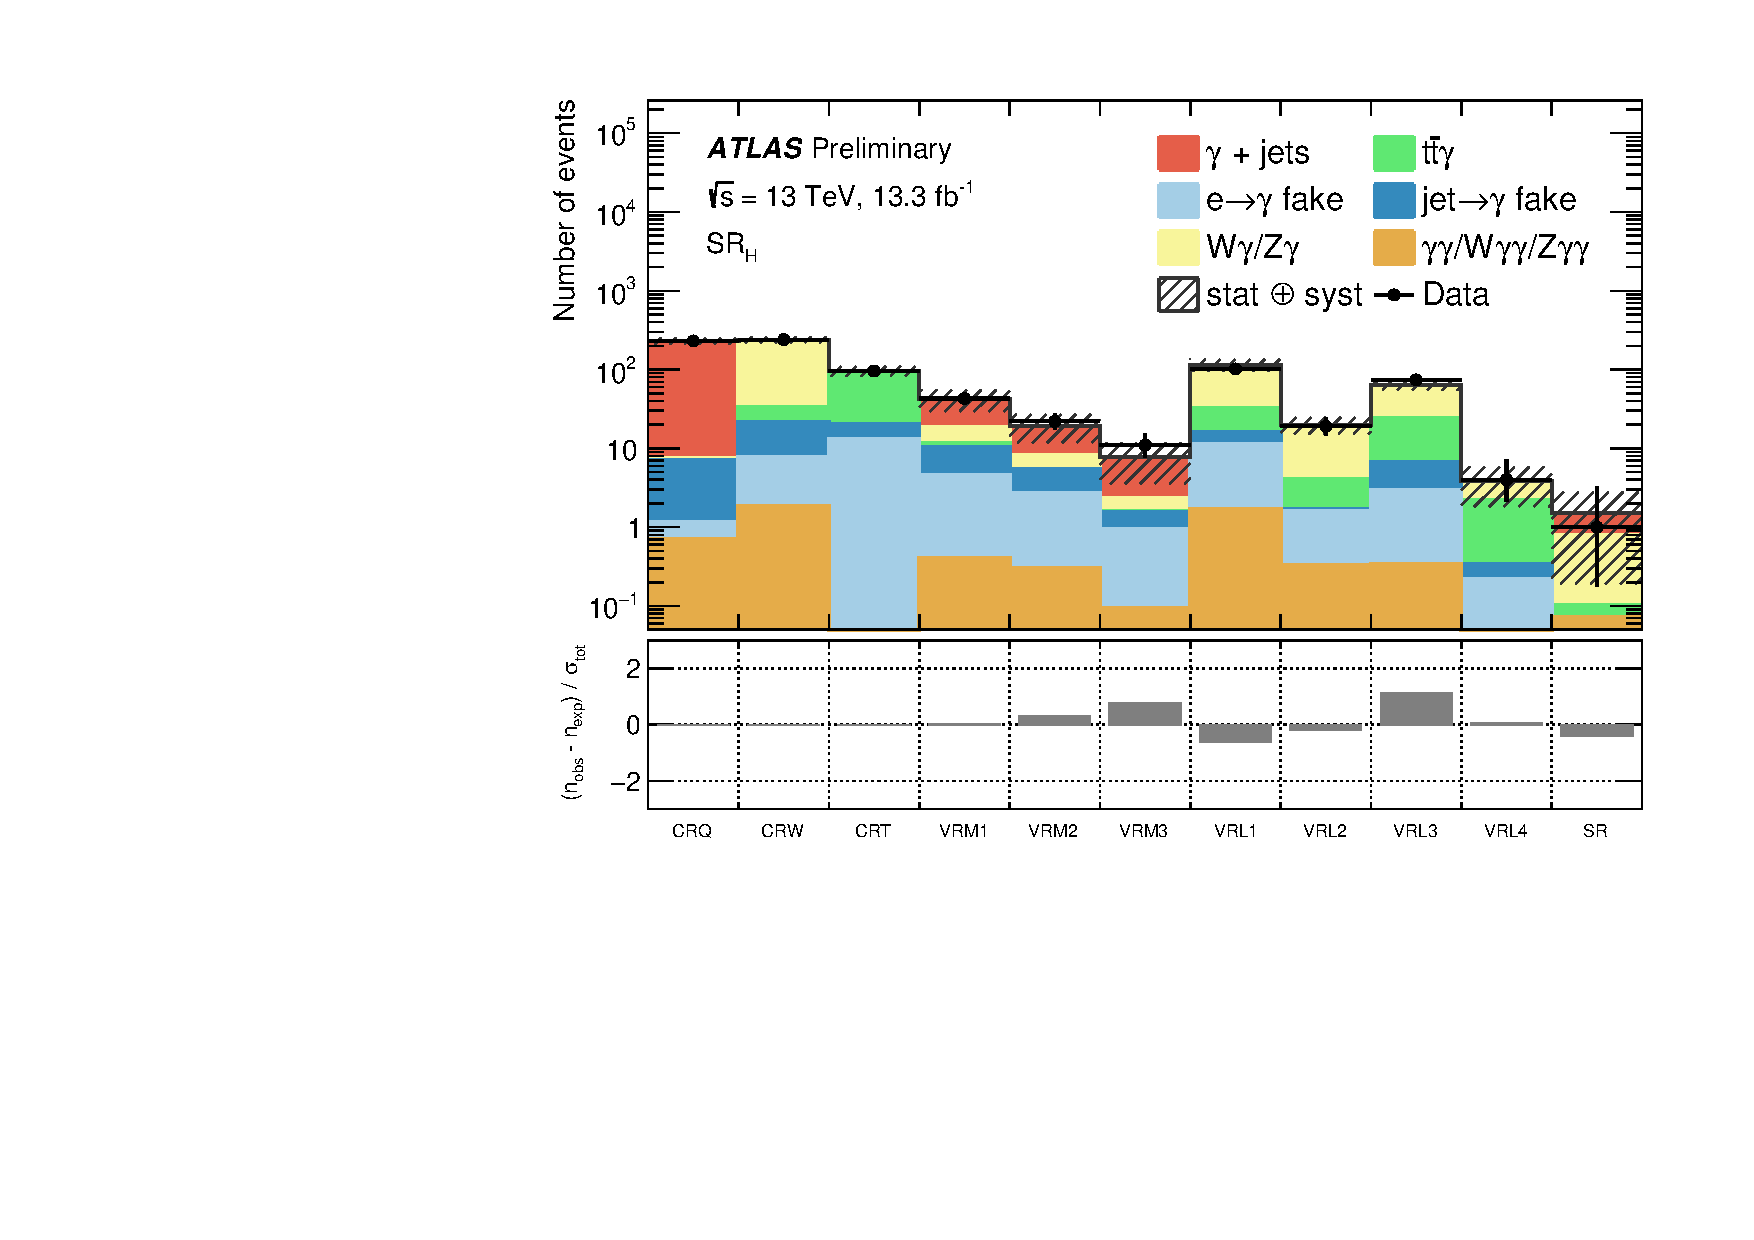
\includegraphics[scale=0.40]{SRH.pdf}
	\end{subfigure}

	\caption{Número de eventos medidos y esperados para las distintas regiones de validación, control y señal, optimizadas para la búsqueda de neutralinos poco masivos (SR$_{\text{L}}$, izquierda) y neutralinos muy masivos (SR$_{\text{H}}$, derecha). El gráfico incluye incertezas estadísticas y sistemáticas \cite{ATLAS:2016fks}.}
\label{SRL_SRH}
\end{figure}


\begin{table}
\centering
\caption{Número de eventos observados y estimación de fondos para las regiones de señal SR$_{\text{L}}$ y SR$_{\text{H}}$ con $13.3 \: \text{fb}^{-1}$ de colisiones $pp$ a $\sqrt{s}=13\etev$\cite{ATLAS:2016fks}.}
\begin{tabular}{ l r r }

	\hline

	Regiones de señal & SR$_{\text{L}}$ &  SR$_{\text{H}}$ \\

	\hline

	Eventos observados & 3 & 1 \\

	\hline

	Eventos esperados por el SM & $0.78 \pm 0.18$ & $1.49 \pm 0.45$\\

	\hline

	$\gamma$ + jets & $0.18 \pm 0.11$ & $0.70 \pm 0.24$\\

	$W\gamma$ & $0.30 \pm 0.07$ & $0.37 \pm 0.09$\\

	$Z\gamma$ & $0.08 \pm 0.08$ & $0.32 \pm 0.32$\\

	$\ttbar\gamma$ & $0.10 \pm 0.04$ & $0.03 \pm 0.01$\\

	$e\rightarrow\gamma$ falsos & $0.07 \pm 0.03$ & $0.00 \pm 0.00$\\

	$j\rightarrow\gamma$ falsos & $0.04 \pm 0.01$ & $0.00 \pm 0.00$\\

	$\gamma\gamma / W\gamma\gamma / Z\gamma\gamma$ & $0.01 \pm 0.00$ & $0.07 \pm 0.01$\\

	\hline


\end{tabular}
\label{ta:SRL_SRH}
\end{table}



\clearpage

\chapter{Electrones identificados como fotones}\label{ch:e_fake}
\chaptermark{Electrones identificados como fotones}


Como ya se mencionó anteriormente, existe un fondo que contribuye a procesos asociados a fotones, jets y energía perdida como estado final, donde un electrón del estado final es identificado como un fotón. Este puede provenir de procesos del SM, como los que producen bosones $W$ y $Z$ + jets, y $\ttbar$. El mismo es difícil de estimar a partir de simulaciones, ya que depende en gran medida de la estructura y material del detector que es muy compleja de modelar en todos sus detalles. El objetivo es entonces estimar este fondo calculando un factor de identificación errónea (\textit{Fake Factor}) en función de las variables $\eta$ y $p_{T}$ de los objetos, a partir de los datos adquiridos por el detector ATLAS durante la toma de datos de 2015 y 2016.

\section{Determinación del factor de identificación errónea}

El método para la estimación del factor de identificación errónea, hace uso de la muestra de eventos $Z\rightarrow ee$. En base a esta muestra se determinan la relación de eventos de pares electrón-positrón y los paras electrón(positrón)-fotón cuya masa invariante es compatible con la del bosón $Z$. Estos últimos pares así seleccionados provienen de eventos en los cuales un electrón (positrón) del decaimiento del $Z$ es reconstruido como un fotón. El factor de identificación espuria se puede calcular entonces como: 

\begin{equation}
F_{e\rightarrow\gamma}[\eta , p_{T}]=\frac{N^{e\gamma}[\eta , p_{T}]}{N^{ee}[\eta , p_{T}]} \label{eq:ff_ratio}
\end{equation}

\noindent
donde $N^{e\gamma}$ y $N^{ee}$ son la cantidad de pares $e\gamma$ y $ee$ respectivamente, con un cierto $\eta$ y $p_{T}$ de uno de sus objetos convenientemente seleccionados.

Los criterios para seleccionar los objetos de los pares de partículas mencionados se explican a continuación y se basan en criterios de selección que mantengan una alta pureza de la muestra, manteniendo un bajo rechazo de señal.
Los electrones  son seleccionados con $p_{T} > 25 \egev$, con un criterio de calidad tanto \textit{tight} como \textit{medium}, y punto de trabajo de aislamiento \textit{gradient loose} \cite{ATLAS-CONF-2016-024}. Para los fotones los requisitos son $p_{T} > 25 \egev$, \textit{tight} y aislados \cite{STDM-2010-08}. A ambos se les solicita que tengan un $\eta_{BE}(2)<2.37$; que estén fuera de la región del \textit{crack} entre $1.37$ y $1.52$; que provengan del vértice primario en base a un parámetro de impacto $d_{0}$ con una significancia menor a 5, y que cumplan con la relación $|\Delta z_{0}\sin\theta|<0.5$ mm.

Además, si un electrón y un fotón son reconstruidos con $\sqrt{\Delta\phi^{2}+\Delta\eta^{2}}<0.4$, el fotón es descartado del evento. Esto reduce precisamente la probabilidad de utilizar candidatos donde un electrón es reconstruido como fotón. Para reducir la contaminación de fondo de $W (\rightarrow e\nu)$ se aplica finalmente un selección de eventos con $\met < 40 \egev$. 


A todos los pares se les solicita una masa invariante entre $75$ y $105 \egev$  estando así en la región de cercanía a la masa del $Z$ ($91.1876 \pm 0.0021 \egev$\cite{Olive:2016xmw}). En el caso de que existiese más de un par en el evento, se utiliza el que tiene la masa invariante más cercana a la del bosón $Z$ . Esto minimiza la contaminación de pares aleatorios, descartando solo unos pocos eventos donde pueda haber más de un $Z$ en estado final.


El primer paso del método consiste en crear un arreglo bidimensional en $\eta$ y $p_{T}$ de los objetos seleccionados. Para eventos positrón-electrón una entrada se realiza para cada partícula en dicho arreglo. En los casos de pares electrón-fotón un arreglo es creado por separado y solo los valores de los fotones son utilizados. 

La concepción del método proviene de la siguiente consideración. Sea $\epsilon_{i}$ la eficiencia de reconstruir un electrón, con un valor de $\eta$ y $p_{T}$ correspondientes al bin \textit{i} del arreglo, para una muestra de \textit{N} pares de electrones y positrones reales (dentro del rango de masa), se determina a $f_{ij}$ como la fracción de pares para los cuales el electrón \textit{leading} (\textit{sub-leading}) está dentro del bin \textit{i} (\textit{j}). Considerando solamente electrones-positrones provenientes del decaimiento de un bosón $Z$, el número de eventos en el bin \textit{i} del arreglo $N^{ee}[\eta , p_{T}]$ es entonces:

\begin{equation}
N_{i}^{ee} = \sum_{j}\epsilon_{i}\epsilon_{j}f_{ij}N + \sum_{j}\epsilon_{j}\epsilon_{i}f_{ji}N = \epsilon_{i}N\sum_{j}\epsilon_{j}(f_{ij}+f_{ji})
\end{equation}

De forma análoga, ahora considerando que $p_{i}$ es la proporción de electrones reconstruidos como fotones en el bin \textit{i}, la cantidad de eventos en el bin \textit{i} del arreglo $N^{e\gamma}[\eta , p_{T}]$ es:

\begin{equation}
N_{i}^{e\gamma} = \sum_{j}p_{i}\epsilon_{j}f_{ij}N + \sum_{j}p_{j}\epsilon_{i}f_{ji}N = p_{i}N\sum_{j}\epsilon_{j}(f_{ij}+f_{ji})
\end{equation}

El factor que determina la proporción de electrones reconstruidos como fotones se define finalmente como:

\begin{equation}
F_{e\rightarrow\gamma}[\eta , p_{T}]\equiv\frac{N^{e\gamma}}{N^{ee}}=\frac{p_{i}}{\epsilon_{i}}
\end{equation}

Por ende, el factor, no es la proporción de fotones mal reconstruidos, sino que es el cociente entre esa proporción y la eficiencia de reconstruir un electrón. De esta forma el fondo correspondiente a electrones identificados como fotones resulta:

\begin{equation}
N_{e\rightarrow\gamma}(\eta , p_{T} , ... ) = F_{e\rightarrow\gamma}(\eta , p_{T})\cdot N_{e}(\eta , p_{T} , ...)
\end{equation}
	
\noindent
donde $N_{e}(\eta , p_{T} , ...)$ es el número de electrones en un determinado estado final correspondiente a las distintas regiones correspondientes a la búsqueda de partículas supersimétricas mencionadas en el capítulo anterior. Estos eventos se seleccionan entonces requiriendo un electrón en lugar de un fotón en el estado final, manteniendo fijo el resto de los cortes utilizados para definir la región de estudio. 

La implementación del método se realizó en ROOT \cite{Brun:1997pa} y C++ en base a histogramas bidimensionales. Para cada evento que contiene un par electrón-positrón, en un histograma con bines de $\eta$ y $p_{T}$ ($N^{ee}[\eta , p_{T}]$), se suma una entrada en el bin correspondiente al $\eta$ y $p_{T}$ de cada uno de los electrones. En el caso de que el evento tenga un par electrón-fotón, en otro histograma ($N^{e\gamma}[\eta , p_{T}]$), se suma una entrada en el bin correspondiente al $\eta$ y $p_{T}$ del fotón. Un esquema de este procedimiento se observa en la Figura \ref{grid}. El correspondiente factor se obtiene entonces como en la ecuación \ref{eq:ff_ratio}.

\begin{figure}
\centering
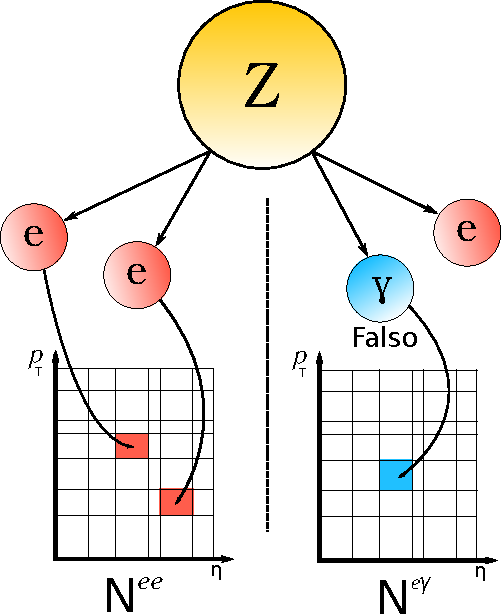
\includegraphics[width=0.45\textwidth]{grid.pdf}
\caption{Procedimiento de llenado de los histogramas $N^{ee}$ y $N^{e\gamma}$ para los pares $ee$ y $e\gamma$.}
\label{grid}
\end{figure}

La muestra de eventos $ee$ y $e\gamma$ colectada no es una muestra pura de $Z$, ya que puede incluir un fondo no resonante en los eventos generados por una combinación aleatoria de objetos o también de eventos de otros procesos electrodébiles, donde los electrones son correctamente reconstruidos o con alguno de los objetos reconstruido erróneamente. Para tener en cuenta la relación entre entradas correspondientes a la señal y las correspondientes al fondo, cada entrada en los histogramas es pesada con un peso representativo de esta relación entre señal y fondo.

% Dado que los pares de objetos utilizados para el cálculo, tienen un probabilidad de no provenir del decaimiento del bosón $Z$, sino de otros procesos no resonantes de fondo, la relación entre señal y fondo tiene en cuenta en el cálculo del factor buscado.
% Para tener en cuenta la relación entre entradas correspondientes a la señal y las correspondientes al fondo, cada entrada en los histogramas es pesada con un peso representativo de esta relación.


\section{Clasificación de eventos}

La relación entre señal y fondo de los eventos correspondientes a la masa del $Z$ se obtiene clasificando a los pares según el tipo ($ee/e\gamma$) y según la región donde se reconstruyeron los objetos \textit{endcap}-\textit{endcap} ($EE$), \textit{barrel}-\textit{endcap} ($BE$) y \textit{barrel}-\textit{barrel} ($BB$). Esto último se debe a que los factores de identificación erróneas dependen de la región del detector donde fueron reconstruidos dados los distinta morfología y tipo de detectores utilizados en cada una ellas. Para cada una de las tres regiones se calcula entonces la masa invariante de los pares, se realiza el correspondiente ajuste para determinar la contribución de señal (S) y fondo (B) y finalmente el peso resulta de la relación:

\begin{equation}
w=\frac{S}{S+B}
\label{eq:peso}
\end{equation}

Los datos utilizados para el presente análisis corresponden a los colectados durante los años 2015 y 2016 del Run 2 del LHC, en base a la denominada derivación EGAM1 (ver Sección \ref{sec:comp_model}) y sin ningún requisito adicional o particular de \textit{triggers}.

Los electrones utilizados para estimar la contaminación de fotones de señal \textit{tight}, pueden pasar tanto requerimientos  \textit{medium} como \textit{tight}. En ambos casos se encuentra una buena relación señal y fondo, siendo naturalmente el caso de selección \textit{tight} la de mayor pureza a costa de una menor estadística de la muestra. Ambas selecciones se estudian en el presente trabajo como se discute en las siguientes secciones.

Para los ajustes de la masas invariantes se utiliza como modelo de señal una \textit{double-sided Crystal-ball} (DSCB) \cite{Das:2016stf}. La misma consiste en una distribución Gaussiana cuyas ramas son reemplazadas por exponenciales. De esta forma se tiene en cuenta efectos gaussianos de resolución en la reconstrucción de los objetos y colas exponenciales que incluyen los efectos de emisión de fotones de bremsstrahlung por parte de los electrones (y sus respectivas técnicas de recuperación \cite{Kartvelishvili:2007zz}). Para el fondo se utiliza como función genérica un polinomio de grado 2. Los resultados de los ajustes obtenidos para cada clasificación de los pares se pueden observar en las Figuras \ref{fits_invmass_medium} y \ref{fits_invmass_tight}. En base a los resultados de estos ajustes se determina la contribución de señal y background en cada región, determinando así los correspondientes pesos (Ecuación \ref{eq:peso}) como se muestra en la Tabla \ref{ta:weights}.

\begin{table}[h]
\centering
\caption{Relación entre señal y fondo (Ecuación \ref{eq:peso}) obtenida para los distintos pares ($ee/e\gamma$) en cada región (EE, BE, BB), para electrones \textit{medium} y \textit{tight}. Las incertezas mostradas son estadísticas.}
\begin{tabular}{ c c c | c c }

	\hline
	\hline

	\multirow{2}{*}{Región} & \multicolumn{2}{c |}{\textit{medium e}} & \multicolumn{2}{c}{\textit{tight e}} \\

	\cline{2-5}

	 & $ee$ & $e\gamma$ & $ee$ & $e\gamma$ \\

	\hline

	EE & 0.915(2) & 0.810(7)  & 0.928(2) & 0.817(7) \\

	BE & 0.937(1) & 0.800(4)  & 0.934(1) & 0.812(5) \\

	BB & 0.9175(7) & 0.722(4)  & 0.9155(8) & 0.734(4) \\

	\hline
	\hline
\end{tabular}
\label{ta:weights}
\end{table}



\section{Incertezas sistemáticas}

% Las principales fuentes de incertezas sistemáticas del método para el cálculo de los factores que determina la contaminación de fondo en las distintas regiones, proviene de las definiciones de las funciones y rangos de ajustes de los fits, así como de las ventanas de aceptación de pares.  Para estimar los posibles incertezas se varió el rango nominal de la masa de $[75-105]\egev$ a los rangos de $[70-110]\egev$ y a $[80-100]\egev$. Como caso extremo en la definición y criterios de ajuste, se determinaron los factores imponiendo los pesos $w=1$ eliminando así la sustracción de fondo en su cálculo. Los resultados de estos estudios se muestran en la Tabla \label{ta:fftable} donde se observa que la incerteza dominante proviene en base al criterio adoptado es la de tomar $w=1$ siendo esta del orden del $20 \%$ dominando sobre todo otra contribución.

Las principales fuentes de incertezas sistemáticas del método para el cálculo de los factores que determina la contaminación de fondo en las distintas regiones, proviene tanto de los ajustes a la masa invariante como de los criterios de aceptación de los pares.  

Para estimar los posibles incertezas se varió el rango nominal de la masa de $[75-105]\egev$ a los rangos de $[70-110]\egev$ y a $[80-100]\egev$. Como caso extremo en la definición y criterios de ajuste, se determinaron los factores imponiendo los pesos $w=1$ eliminando así la sustracción de fondo en su cálculo. 

Los resultados de estos estudios para electrones \textit{medium} y \textit{tight} se muestran en las Tablas \ref{ta:fftable_medium} y \ref{ta:fftable_tight}, donde se observa que la incerteza dominante proviene de tomar $w=1$ siendo esta del orden del $20 \%$ dominando sobre todo otra contribución.

% \begin{table}
% \centering
% \begin{threeparttable}
% \caption{Incertezas sistemáticas de los factores en bines de $\eta$ y $p_{T}$. Se puede observar que el sistemático $w=1$ es el que predomina.}
% \begin{tabular}{ l l c c c }

% 	\hline
% 	\hline

% 	$|\eta|$ & $p_{T}$[GeV] & $w=1$ & Rango & Total \\
% 	\hline

% 	0 - 0.6 	& 75 - 90 	& 0.0155 & 0.0004 & 0.004 \\

% 	0 - 0.6 	& 90 - 145 	& 0.0141 & 0.0004 & 0.004 \\

% 	0 - 0.6 	& 145 - 300 & 0.0116 & 0.0008 & 0.002 \\

% 	\hline

% 	0.6 - 1.37 	& 75 - 90 	& 0.0173 & 0.0004 & 0.004 \\

% 	0.6 - 1.37 	& 90 - 145 	& 0.0161 & 0.0004 & 0.004 \\

% 	0.6 - 1.37 	& 145 - 300 & 0.0121 & 0.0008 & 0.003 \\

% 	\hline

% 	1.52 - 1.82 & 75 - 90 	& 0.036  & 0.001 & 0.00 \\

% 	1.52 - 1.82 & 90 - 145 	& 0.033  & 0.001 & 0.004 \\

% 	1.52 - 1.82 & 145 - 300 & 0.022  & 0.002 & 0.003 \\

% 	\hline

% 	1.82 - 2.37 & 75 - 90 	& 0.046		& 0.001 & 0.007 \\

% 	1.82 - 2.37 & 90 - 145	& 0.039		& 0.001 & 0.006 \\

% 	1.82 - 2.37 & 145 - 300 & 0.041		& 0.003 & 0.006 \\

% 	\hline
% \end{tabular}
% \label{ta:syst}
% \end{threeparttable}
% \end{table}

% Lo mismo se hizo con el rango del fit que se varió de su rango nominal $[70-110]\egev$, a $[65-115]\egev$ y a $[75-105]\egev$. 

% Otro sistemático surgió de la utilización de una función diferente para modelar el fondo, en este caso se usó un polinomio de grado 3. Como caso extremo en la definición y criterios de ajuste, se determinaron los factores imponiendo los pesos $w=1$ eliminando así la sustracción de fondo en su cálculo. 

%Se consideran distintas fuentes de incertezas sistemáticas. Una de ellas proveniente de la variación tanto del rango del fit, como del rango de masa de aceptación de los pares. El rango nominal del fit es $[70-110]\egev$ y se varía a $[65-115]\egev$ y a $[75-105]\egev$. El rango nominal de la masa es $[75-105]\egev$ y se varía a $[70-110]\egev$ y a $[80-100]\egev$. Se tuvo en cuenta también como fuente de sistemático, la variación en los valores de los factores al utilizar otra función para el ajuste del fondo, utilizándose un polinomio de grado 3 y un polinomio de Bernstein de grado 4.



\begin{figure}

	\begin{subfigure}{0.5\textwidth}
		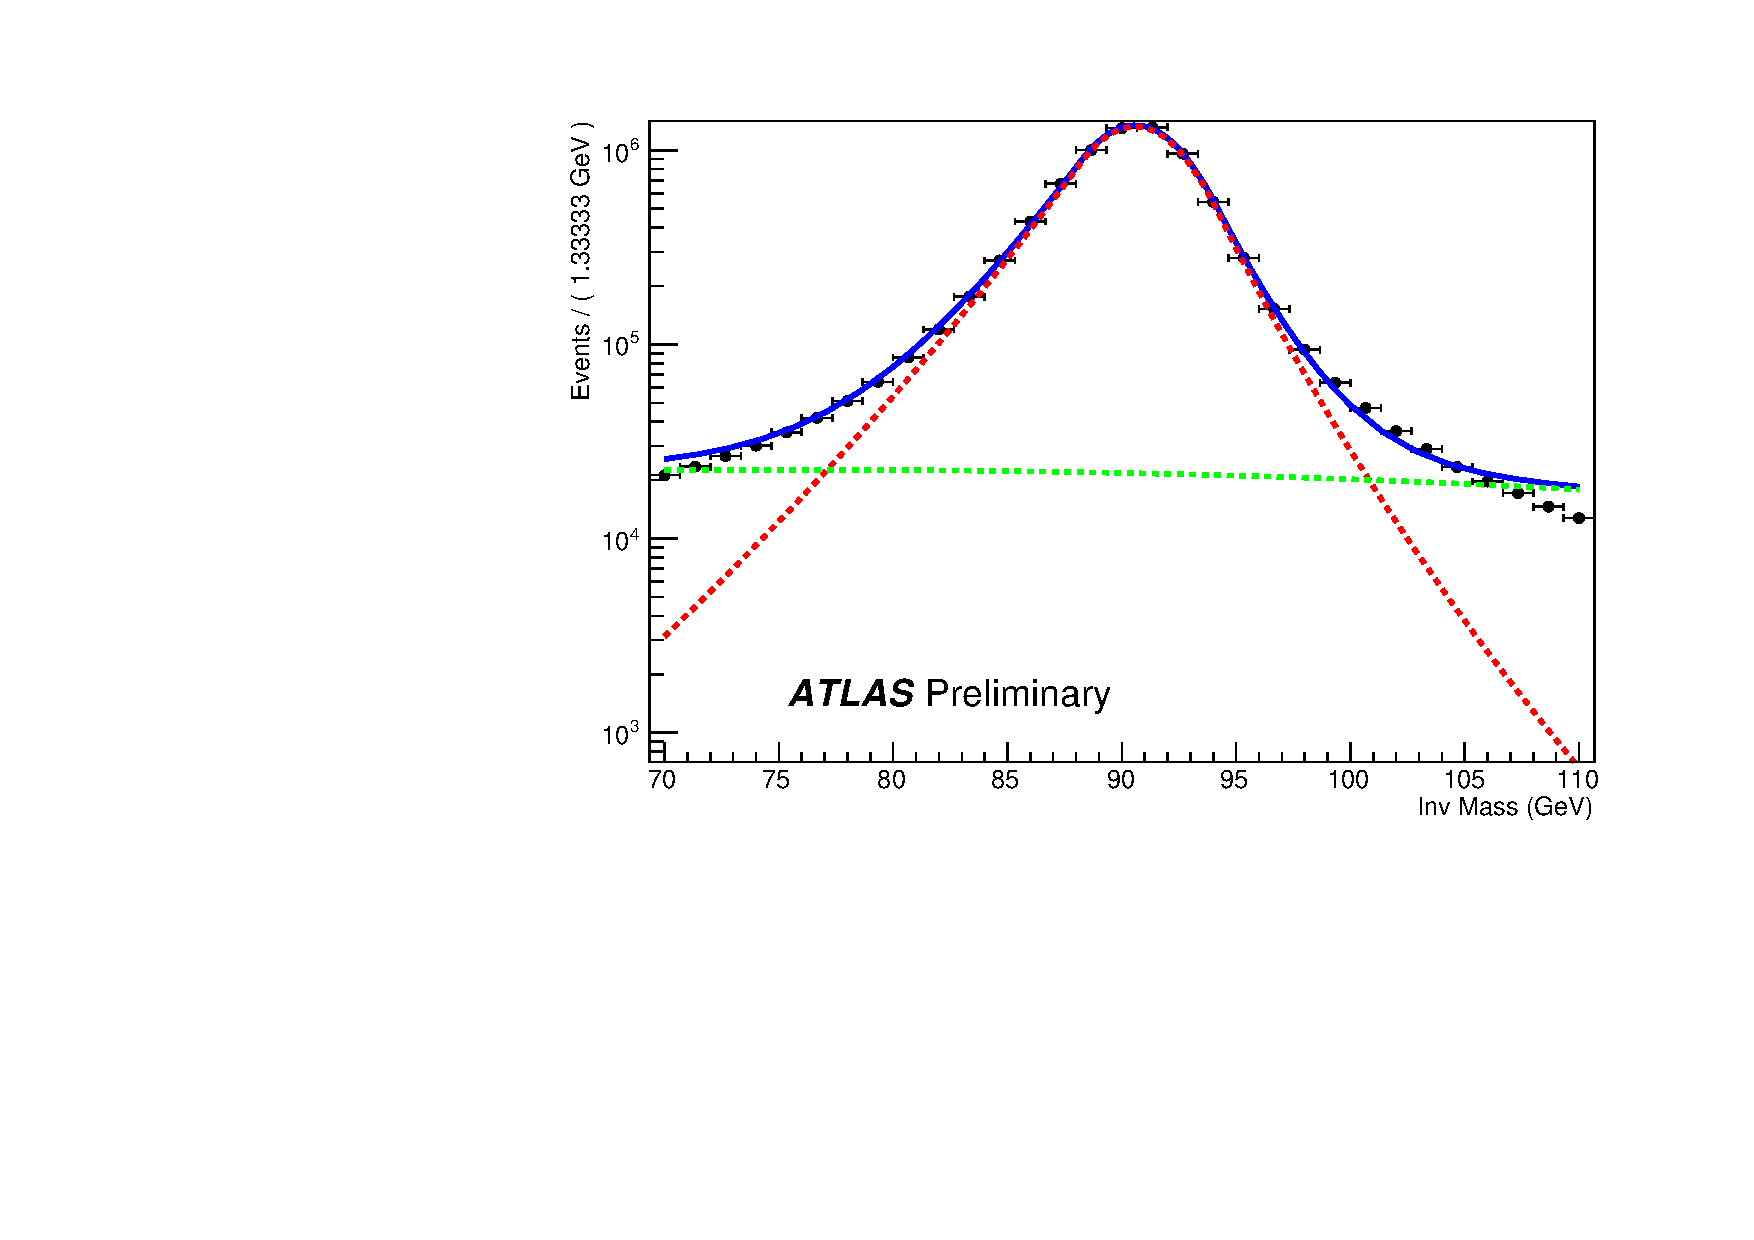
\includegraphics[scale=0.40]{d15_16_egam1_m_lmet_fit_h_m_ee_BB.pdf} 
		\caption{Región BB}
	\end{subfigure}
	~
	\begin{subfigure}{0.5\textwidth}
		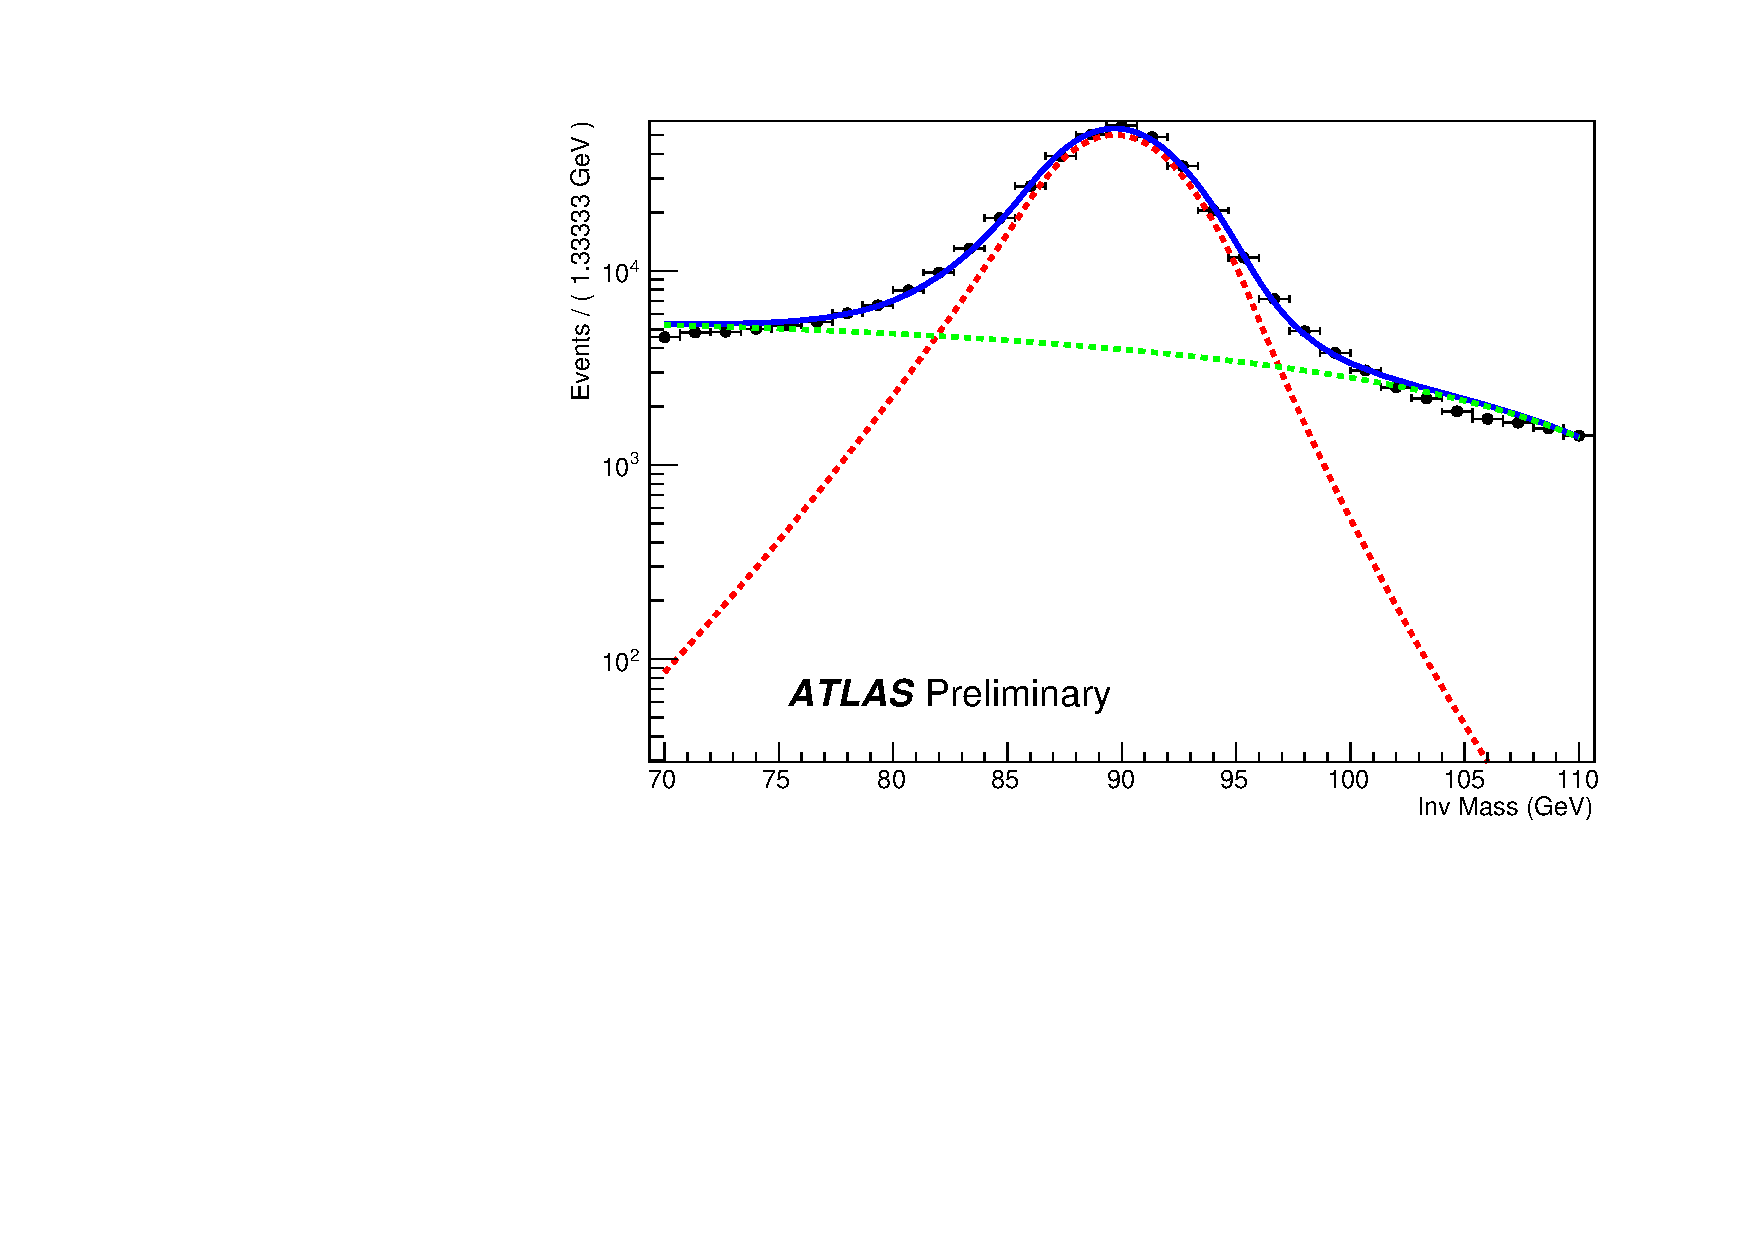
\includegraphics[scale=0.40]{d15_16_egam1_m_lmet_fit_h_m_eg_BB.pdf}
		\caption{Región BB}
	\end{subfigure}
	~
	\begin{subfigure}{0.5\textwidth}
		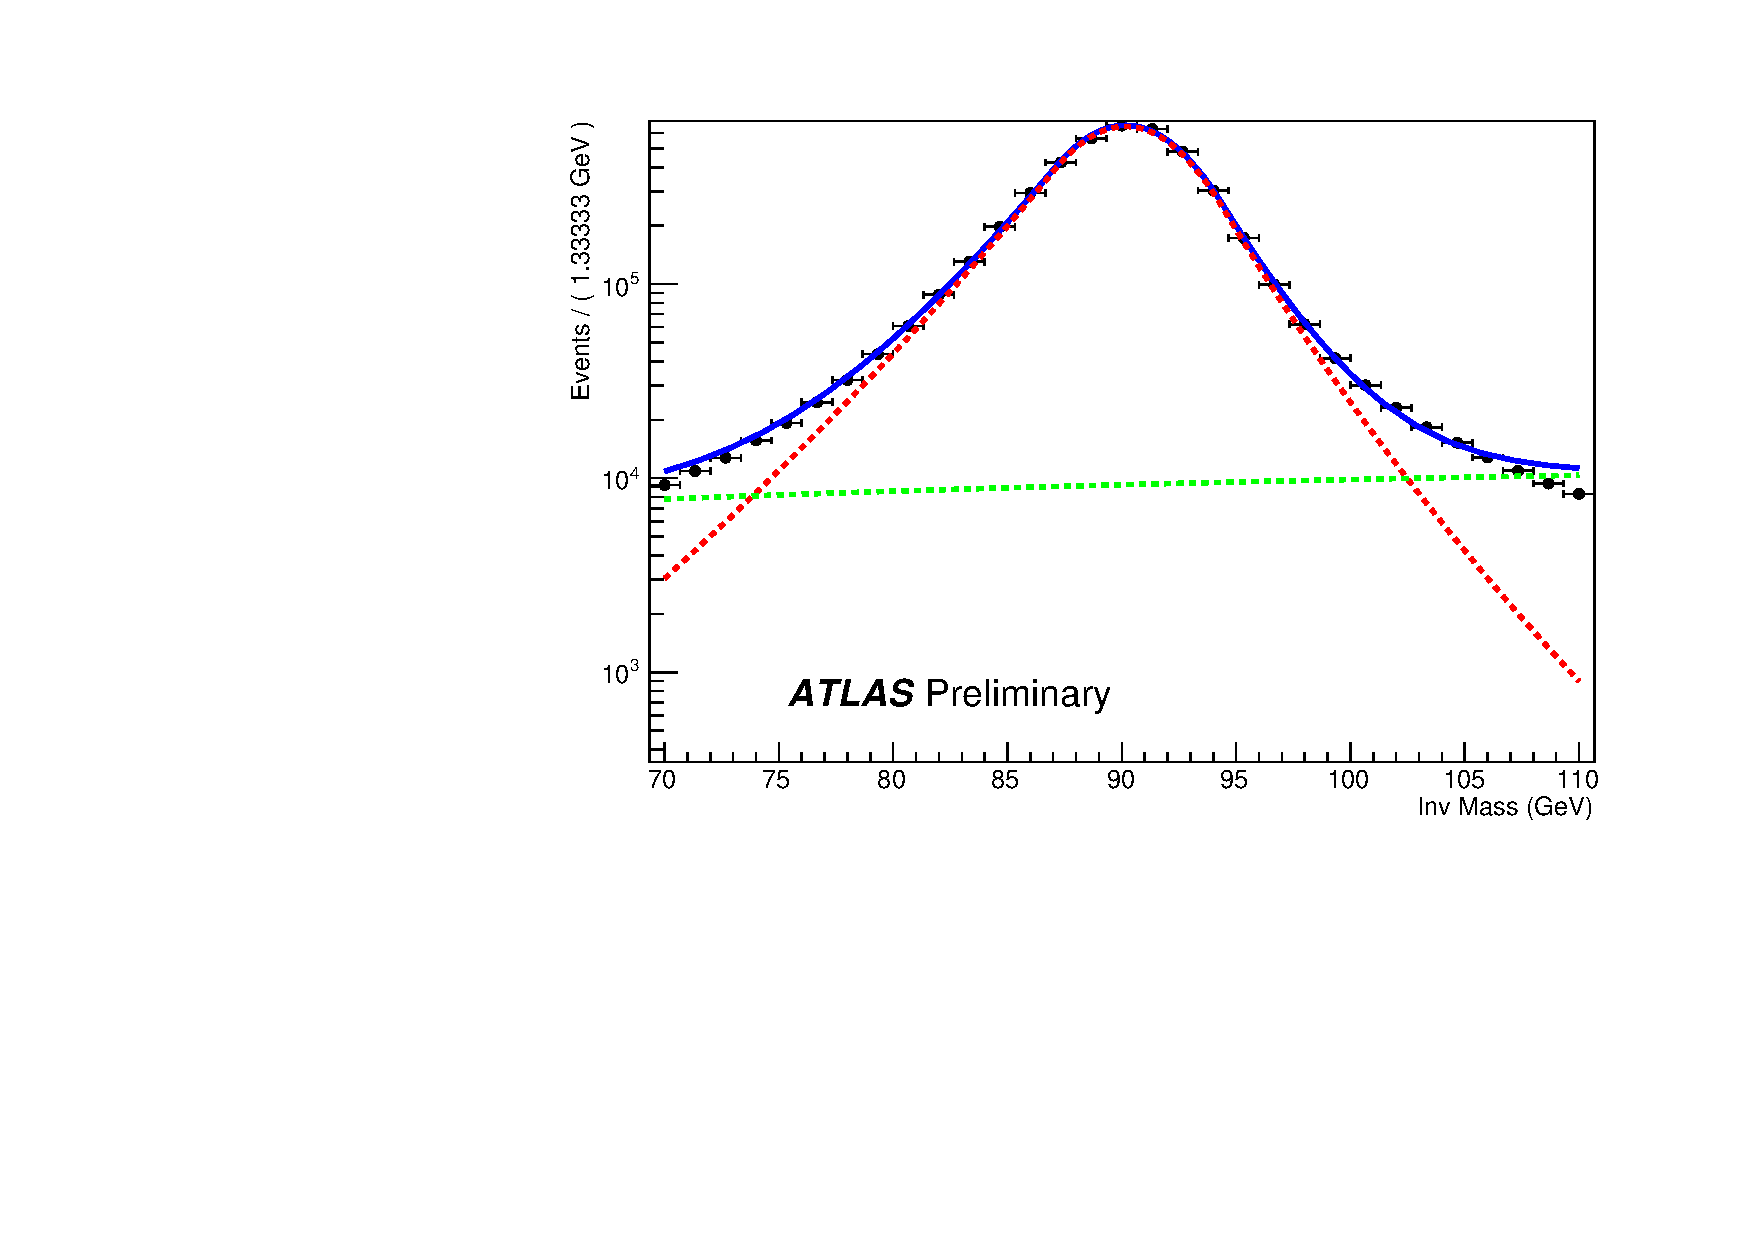
\includegraphics[scale=0.40]{d15_16_egam1_m_lmet_fit_h_m_ee_BE.pdf} 
		\caption{Región BE}
	\end{subfigure}
	~
	\begin{subfigure}{0.5\textwidth}
		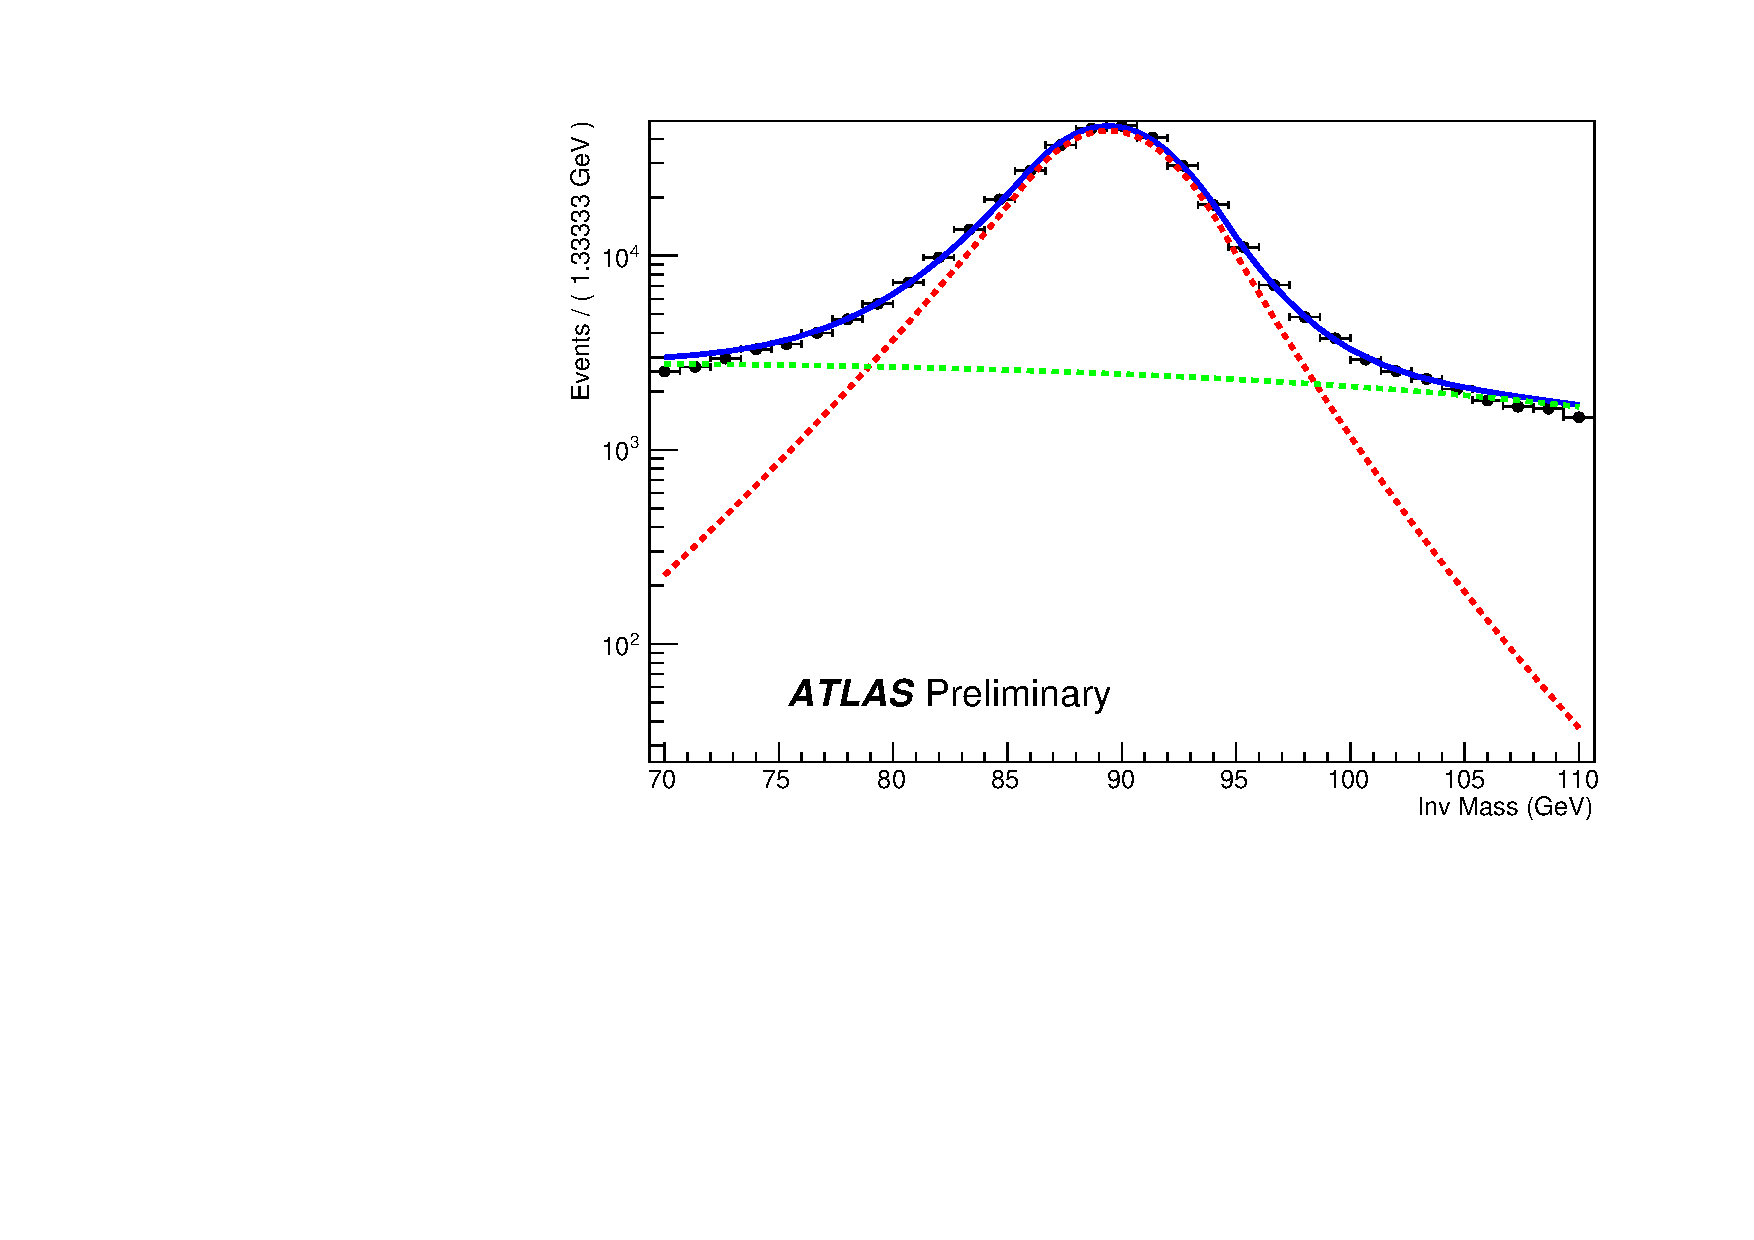
\includegraphics[scale=0.40]{d15_16_egam1_m_lmet_fit_h_m_eg_BE.pdf}
		\caption{Región BE}
	\end{subfigure}
	~
	\begin{subfigure}{0.5\textwidth}
		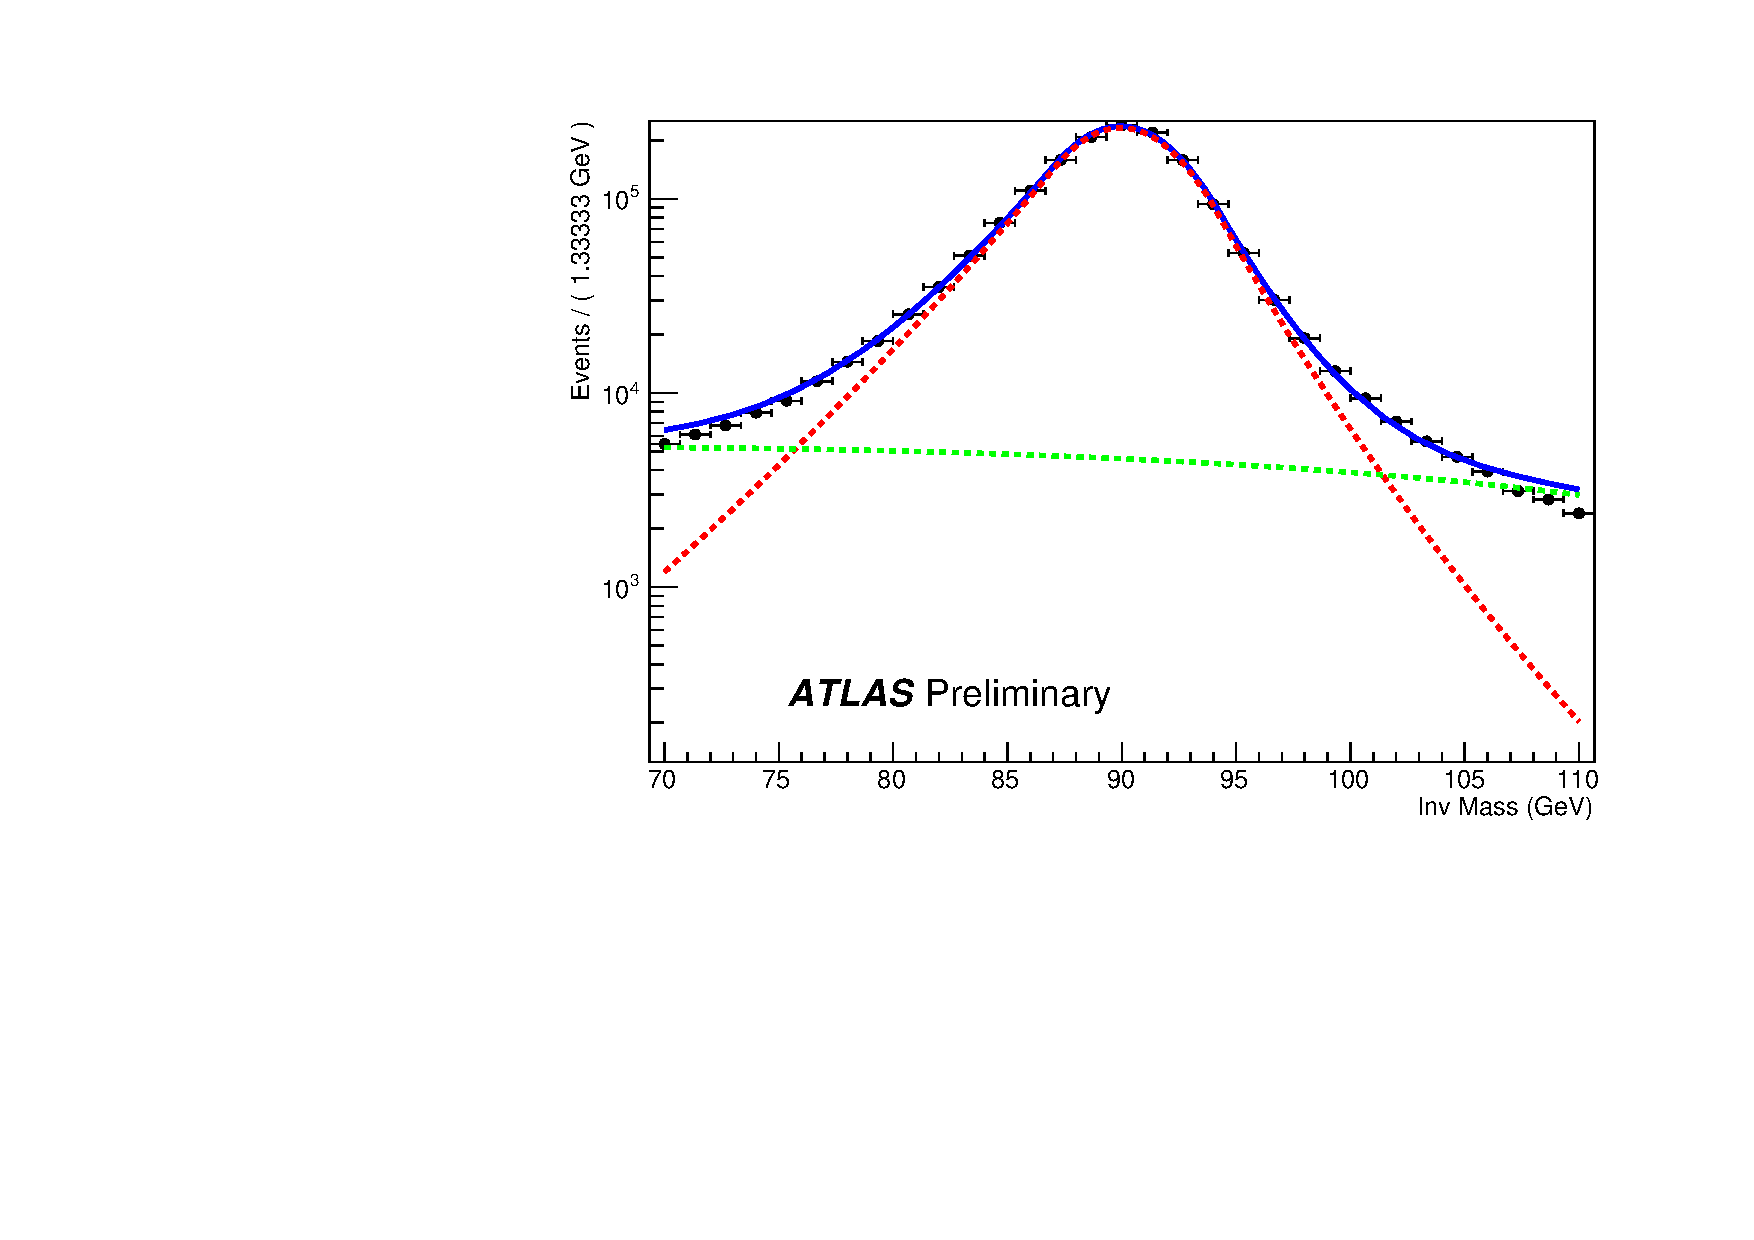
\includegraphics[scale=0.40]{d15_16_egam1_m_lmet_fit_h_m_ee_EE.pdf} 
		\caption{Región EE}
	\end{subfigure}
	~
	\begin{subfigure}{0.5\textwidth}
		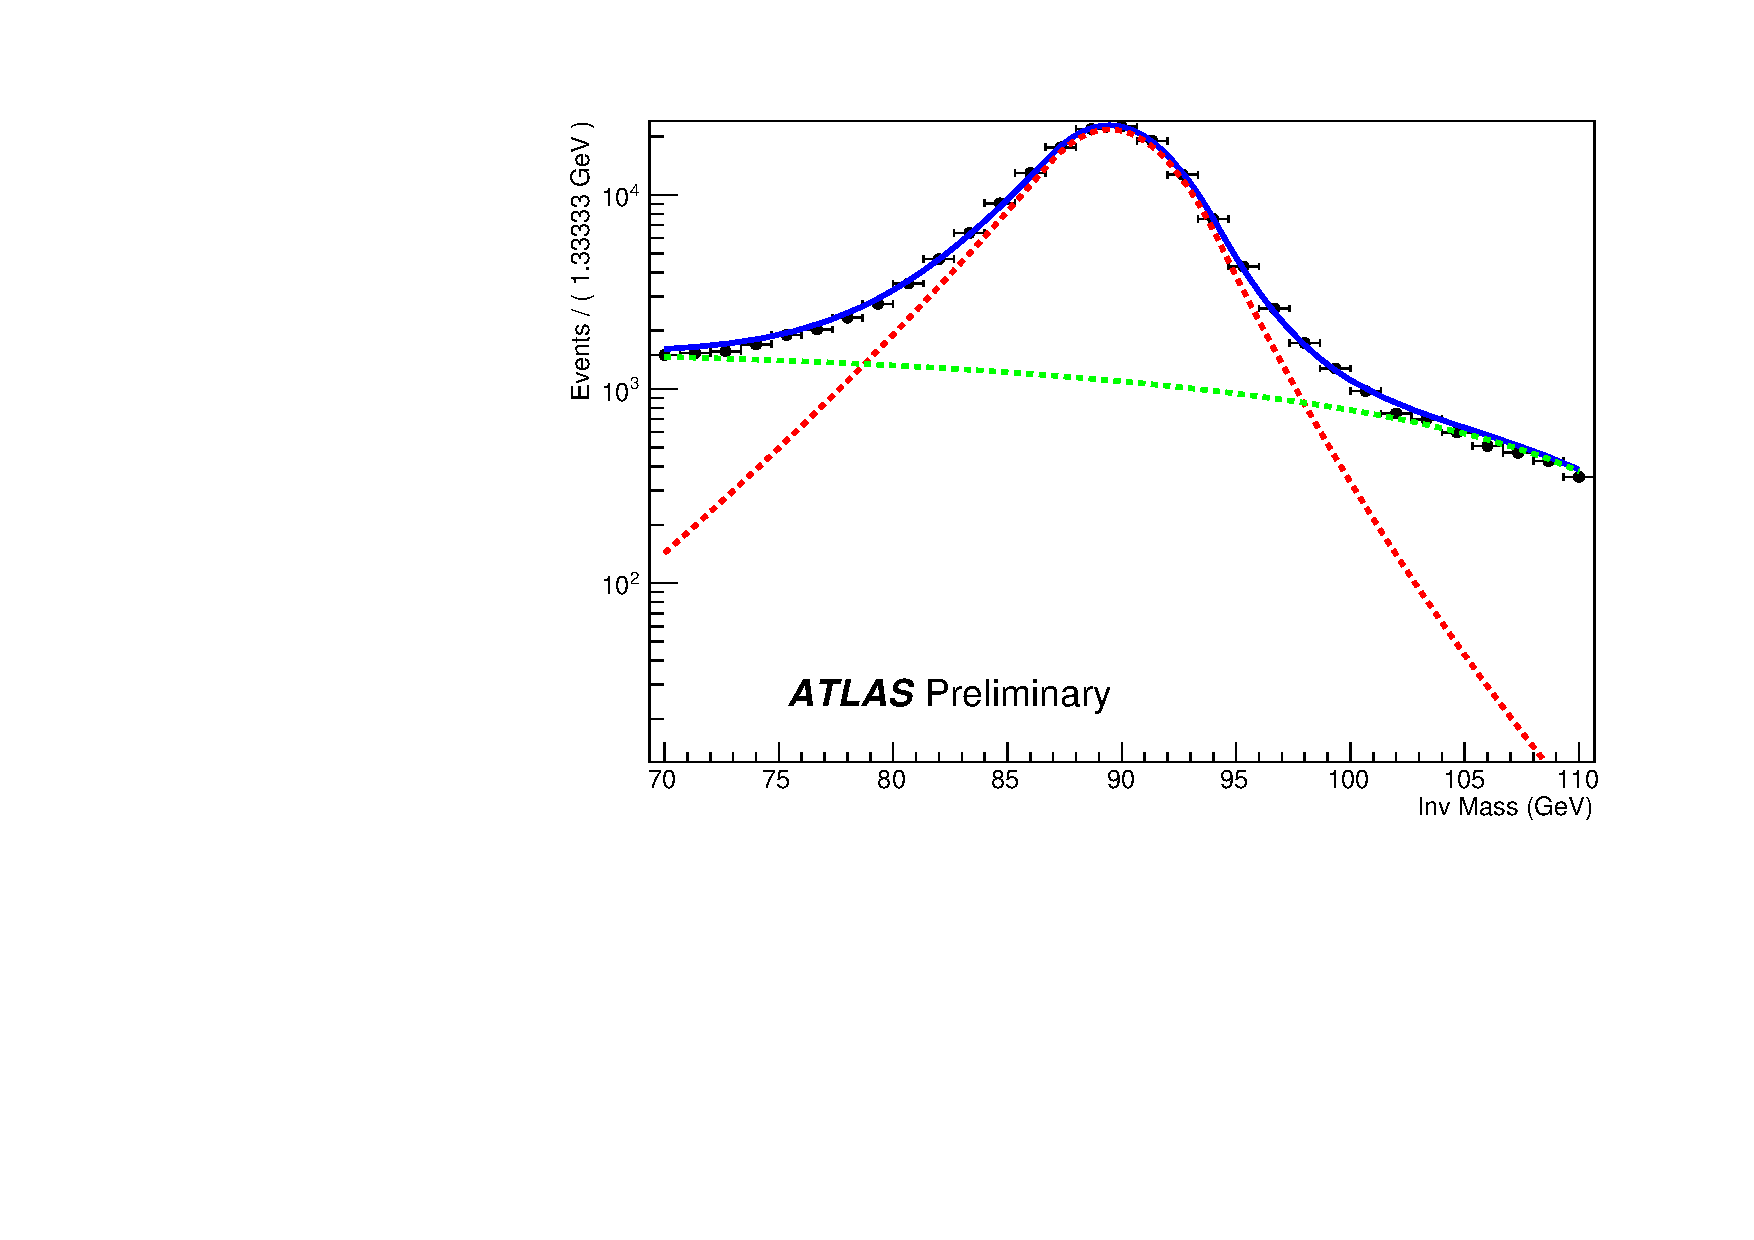
\includegraphics[scale=0.40]{d15_16_egam1_m_lmet_fit_h_m_eg_EE.pdf}
		\caption{Región EE}
	\end{subfigure}

	\caption{Ajuste de la masa invariante de los pares $ee$ (izquierda) y $e\gamma$ (derecha), para cada región de reconstrucción y para electrones \textit{medium}. La curva roja corresponde a la DSCB, la verde al polinomio de grado 2 y la azul a la combinación resultante de ambas.}
\label{fits_invmass_medium}
\end{figure}

\begin{figure}

	\begin{subfigure}{0.5\textwidth}
		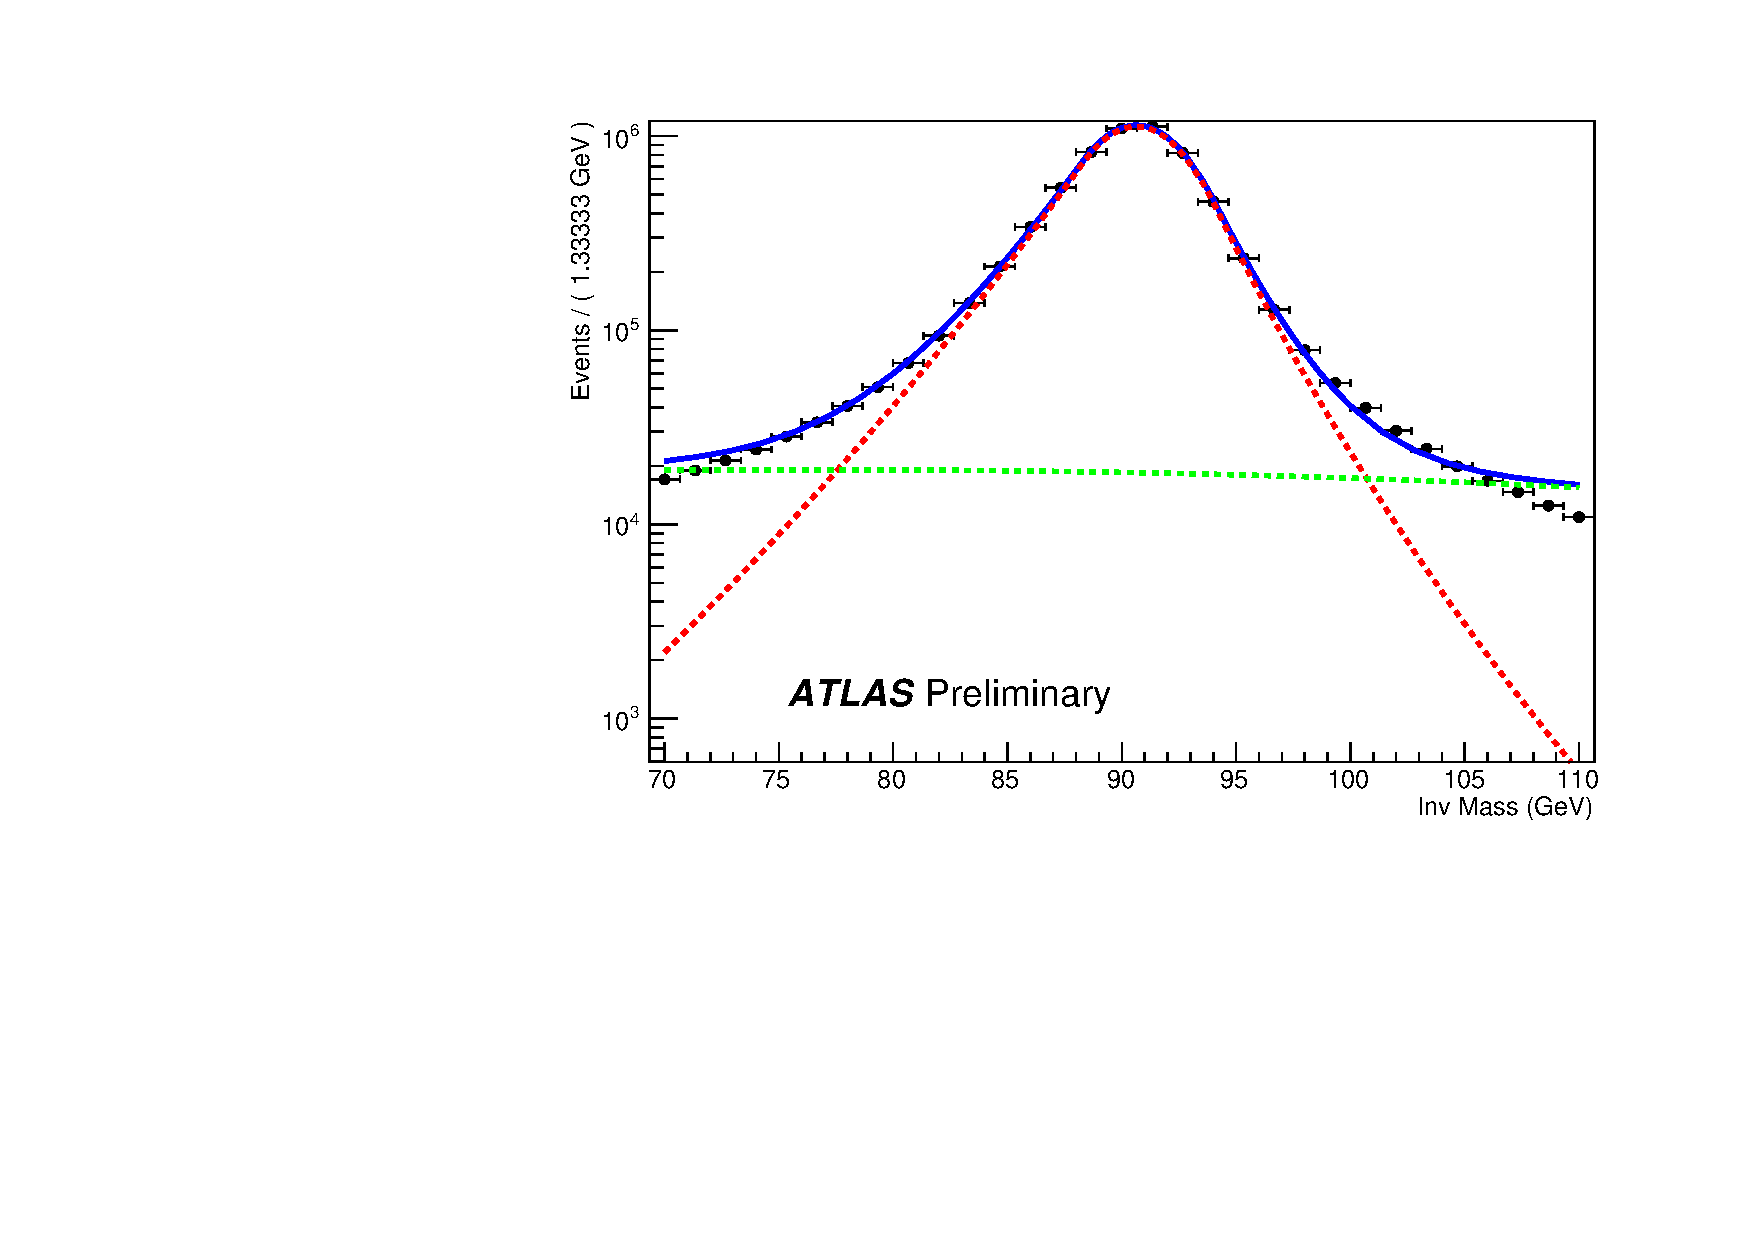
\includegraphics[scale=0.40]{d15_16_egam1_t_lmet_fit_h_m_ee_BB.pdf} 
		\caption{Región BB}
	\end{subfigure}
	~
	\begin{subfigure}{0.5\textwidth}
		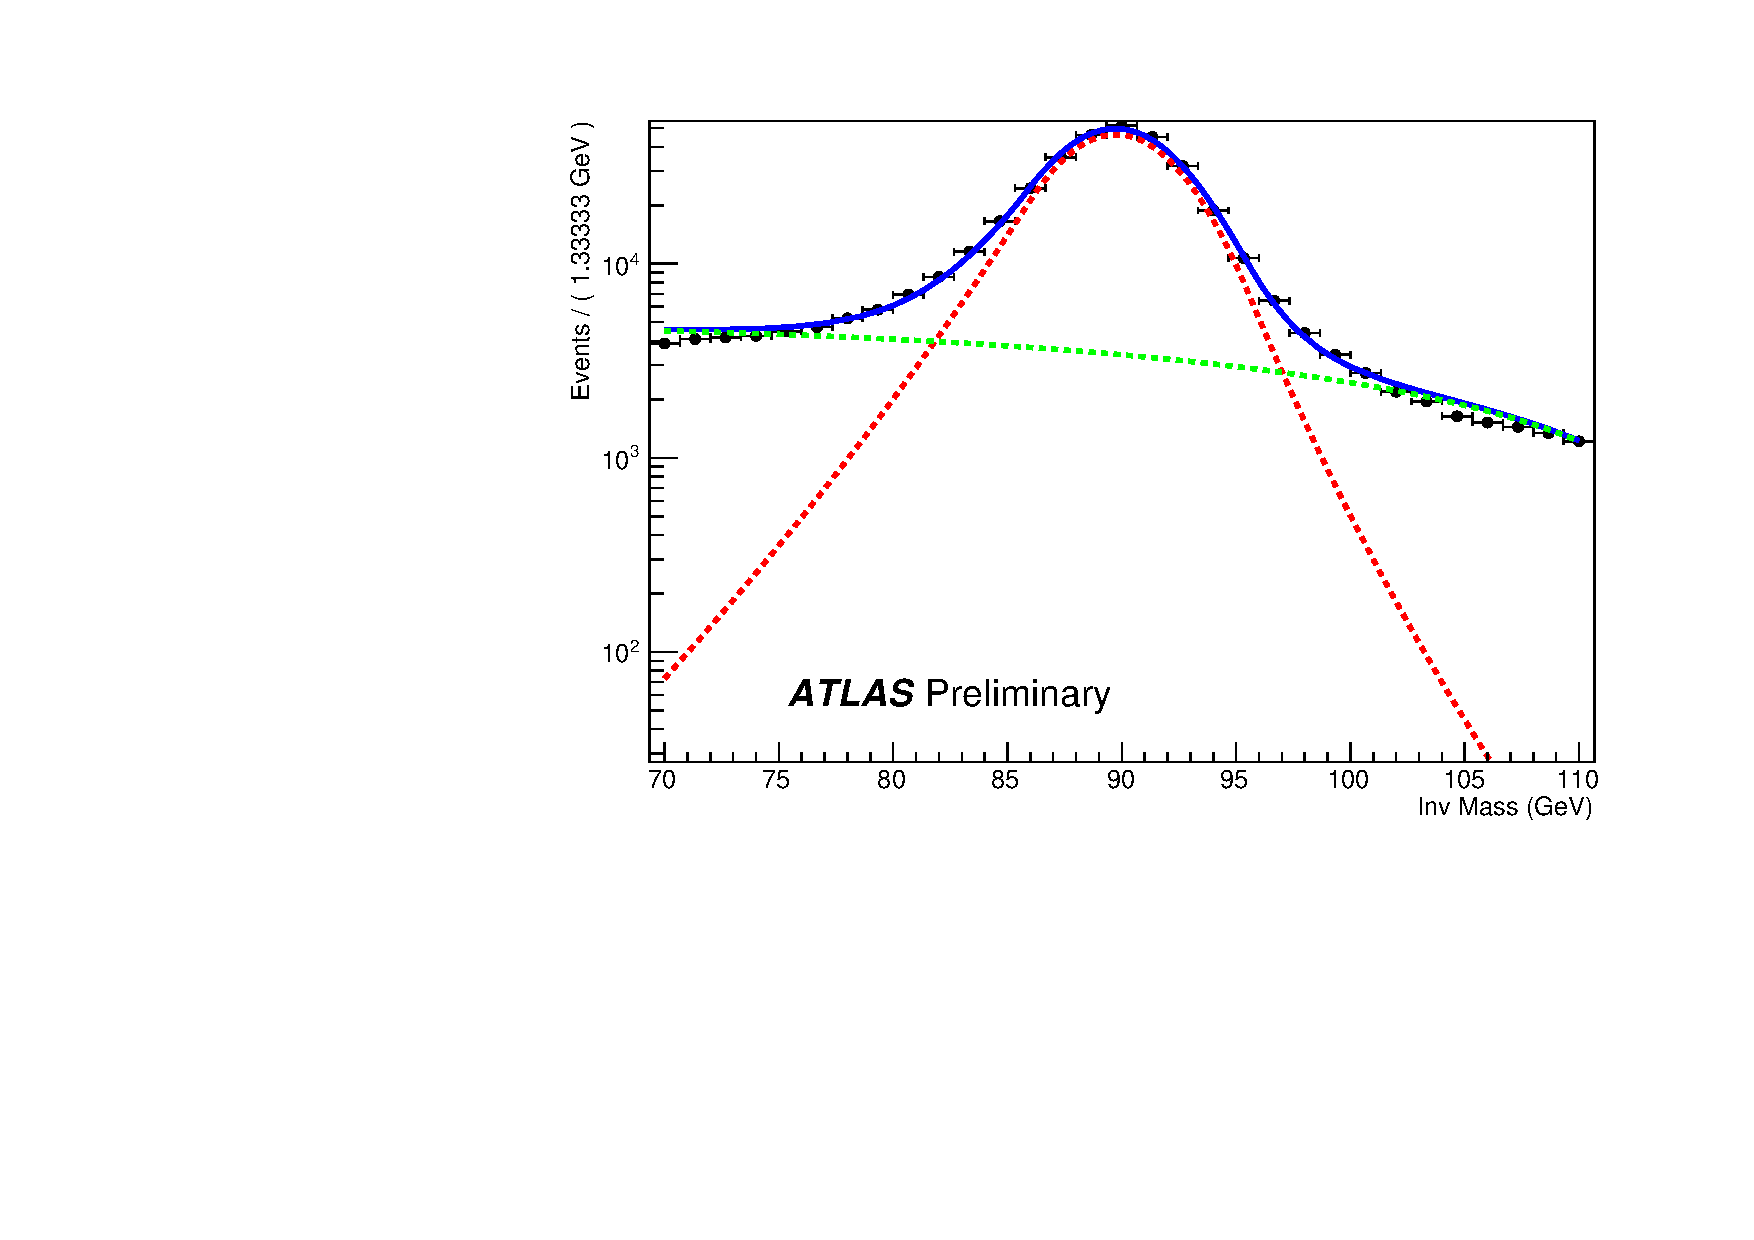
\includegraphics[scale=0.40]{d15_16_egam1_t_lmet_fit_h_m_eg_BB.pdf}
		\caption{Región BB}
	\end{subfigure}
	~
	\begin{subfigure}{0.5\textwidth}
		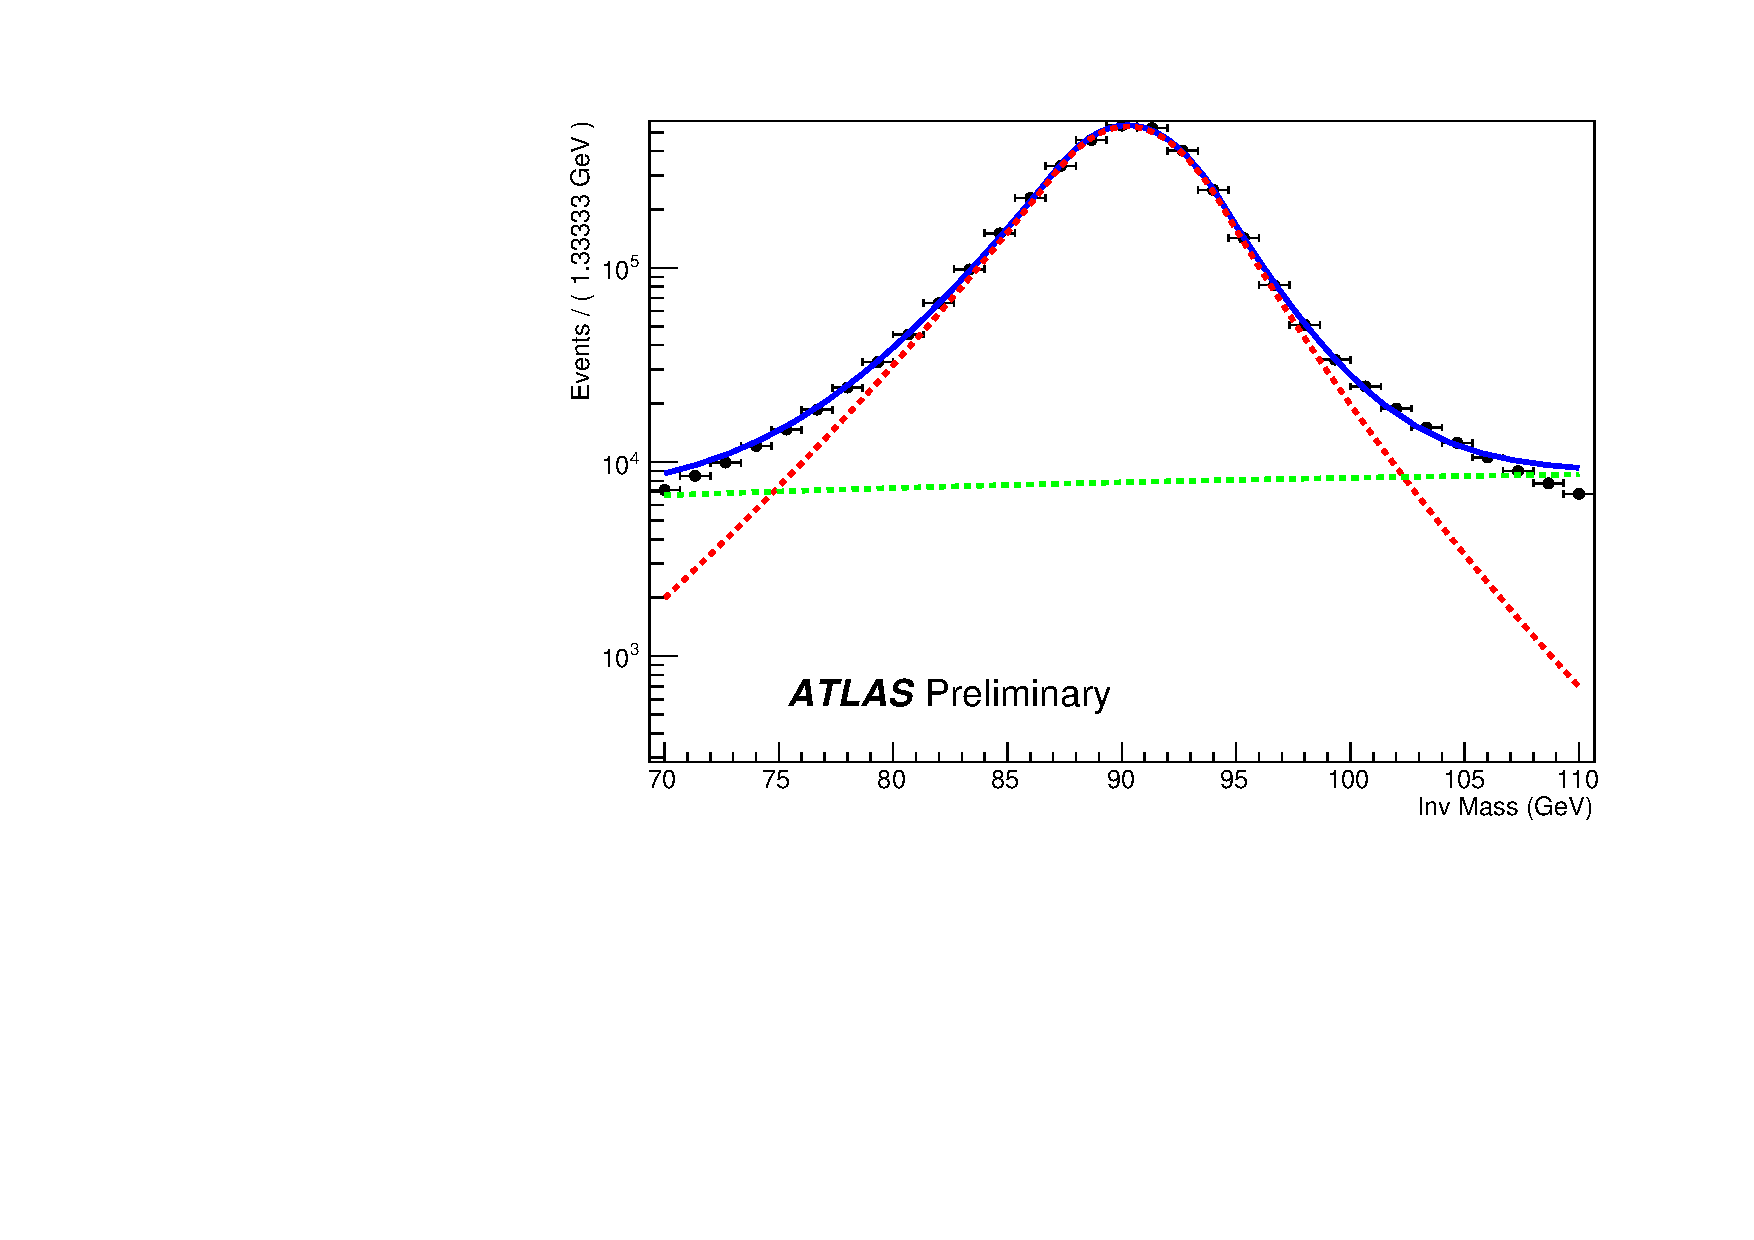
\includegraphics[scale=0.40]{d15_16_egam1_t_lmet_fit_h_m_ee_BE.pdf} 
		\caption{Región BE}
	\end{subfigure}
	~
	\begin{subfigure}{0.5\textwidth}
		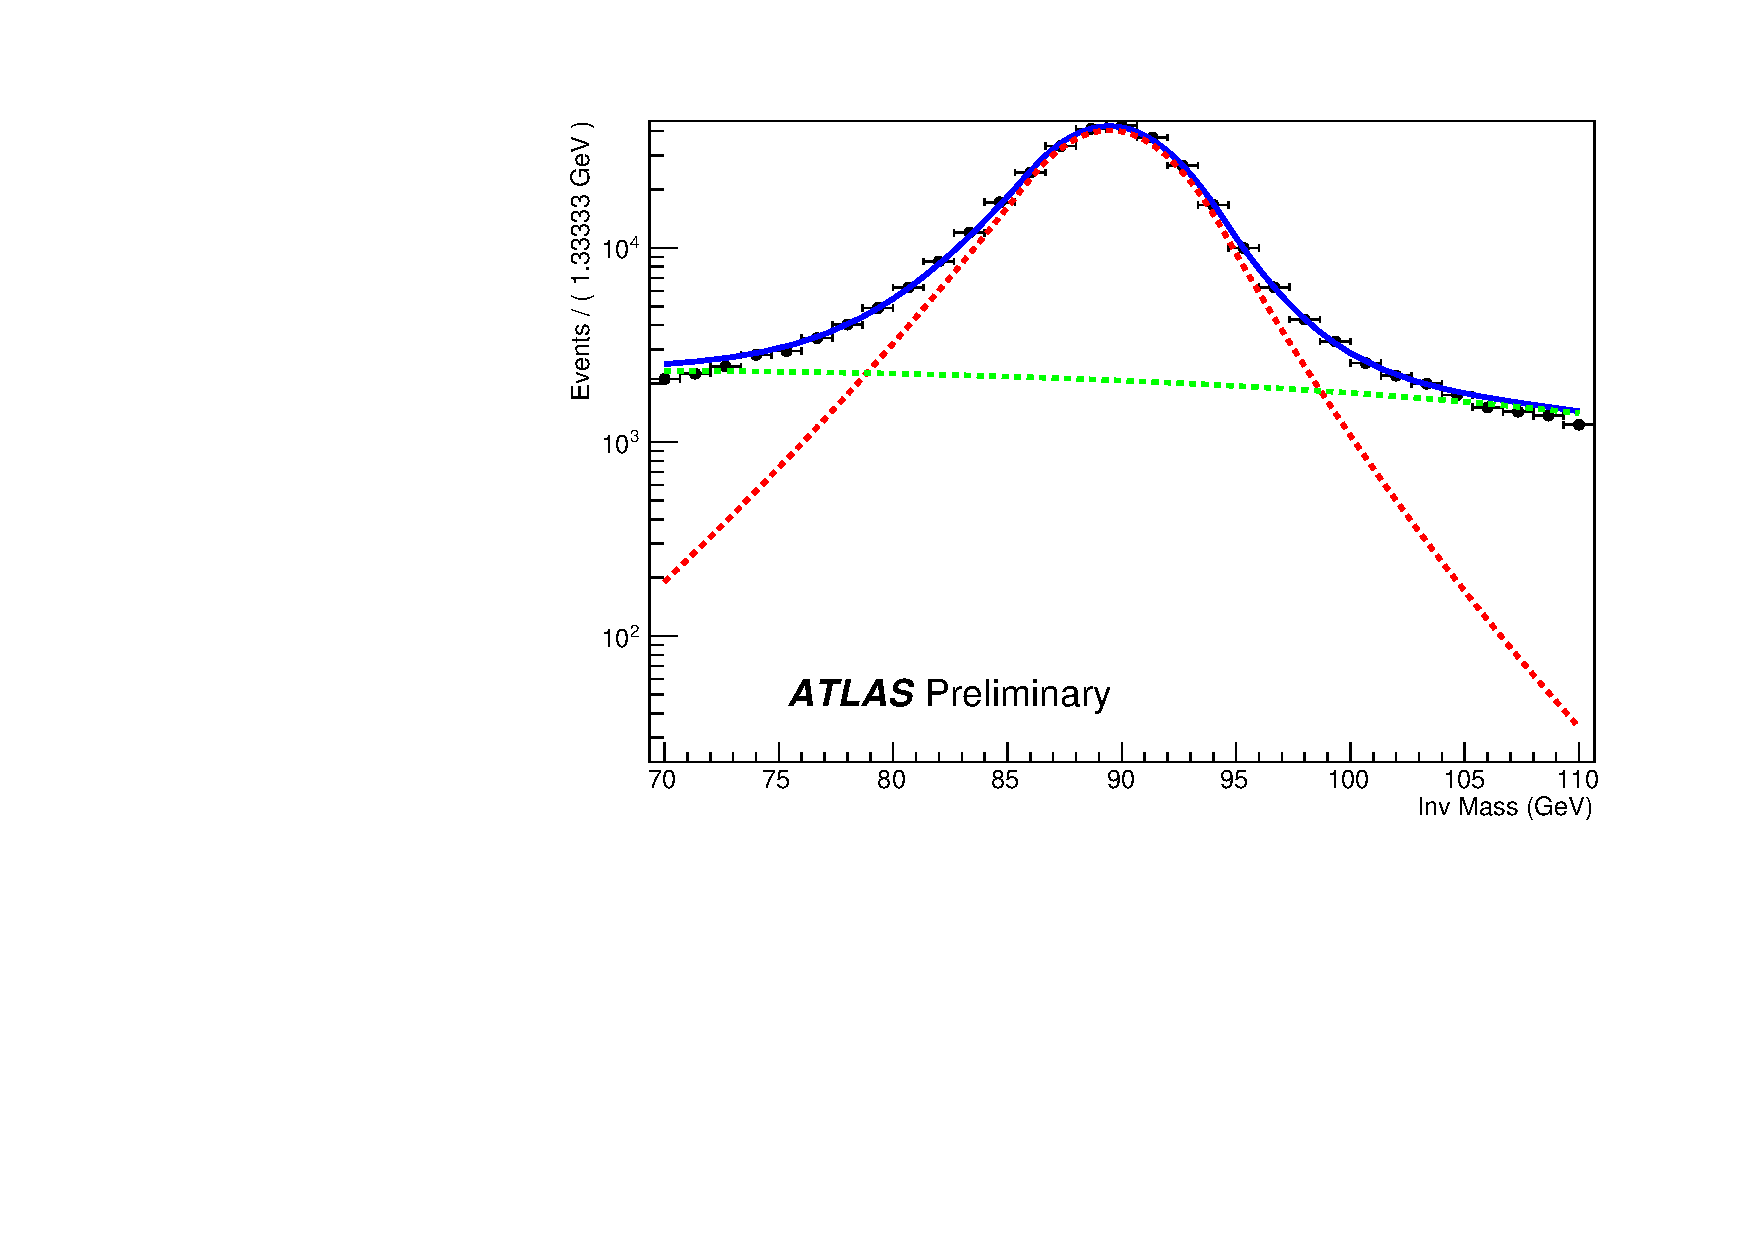
\includegraphics[scale=0.40]{d15_16_egam1_t_lmet_fit_h_m_eg_BE.pdf}
		\caption{Región BE}
	\end{subfigure}
	~
	\begin{subfigure}{0.5\textwidth}
		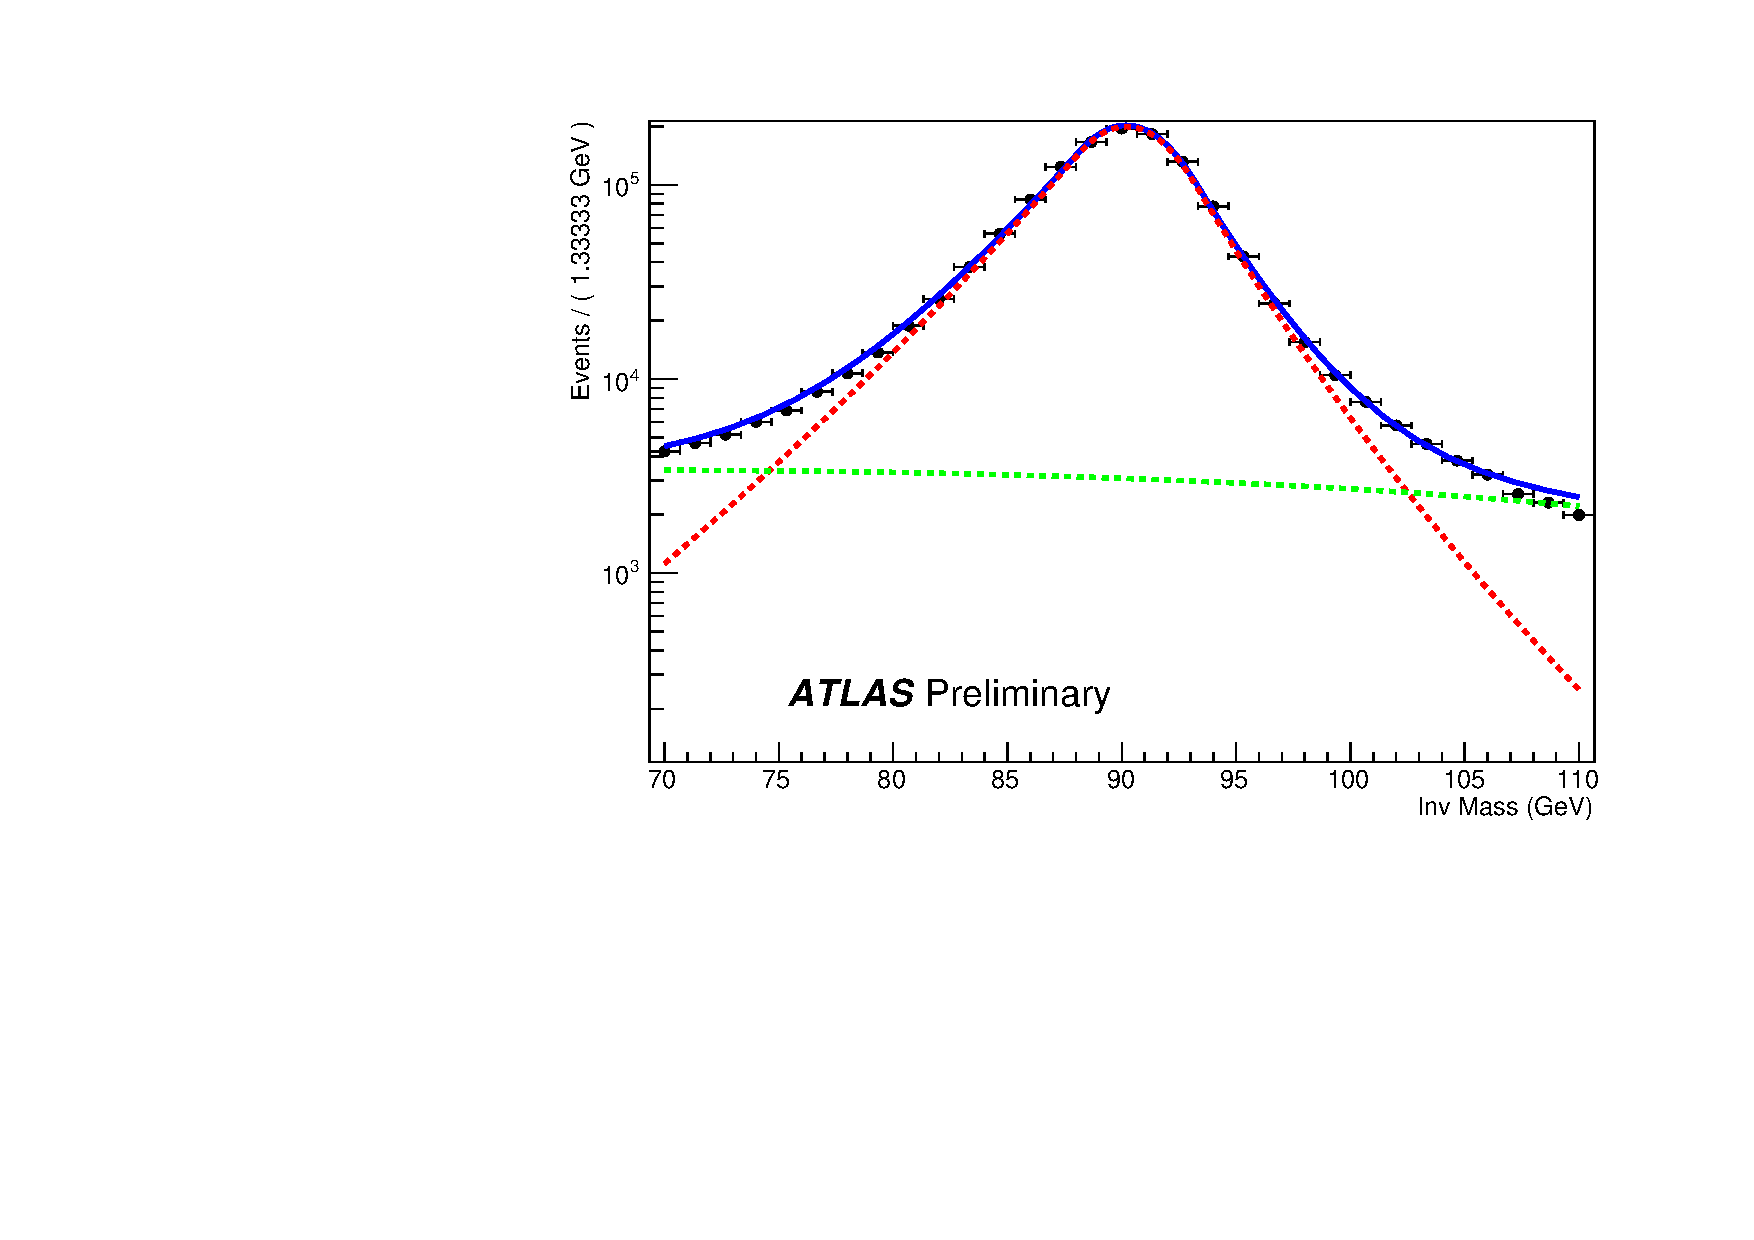
\includegraphics[scale=0.40]{d15_16_egam1_t_lmet_fit_h_m_ee_EE.pdf} 
		\caption{Región EE}
	\end{subfigure}
	~
	\begin{subfigure}{0.5\textwidth}
		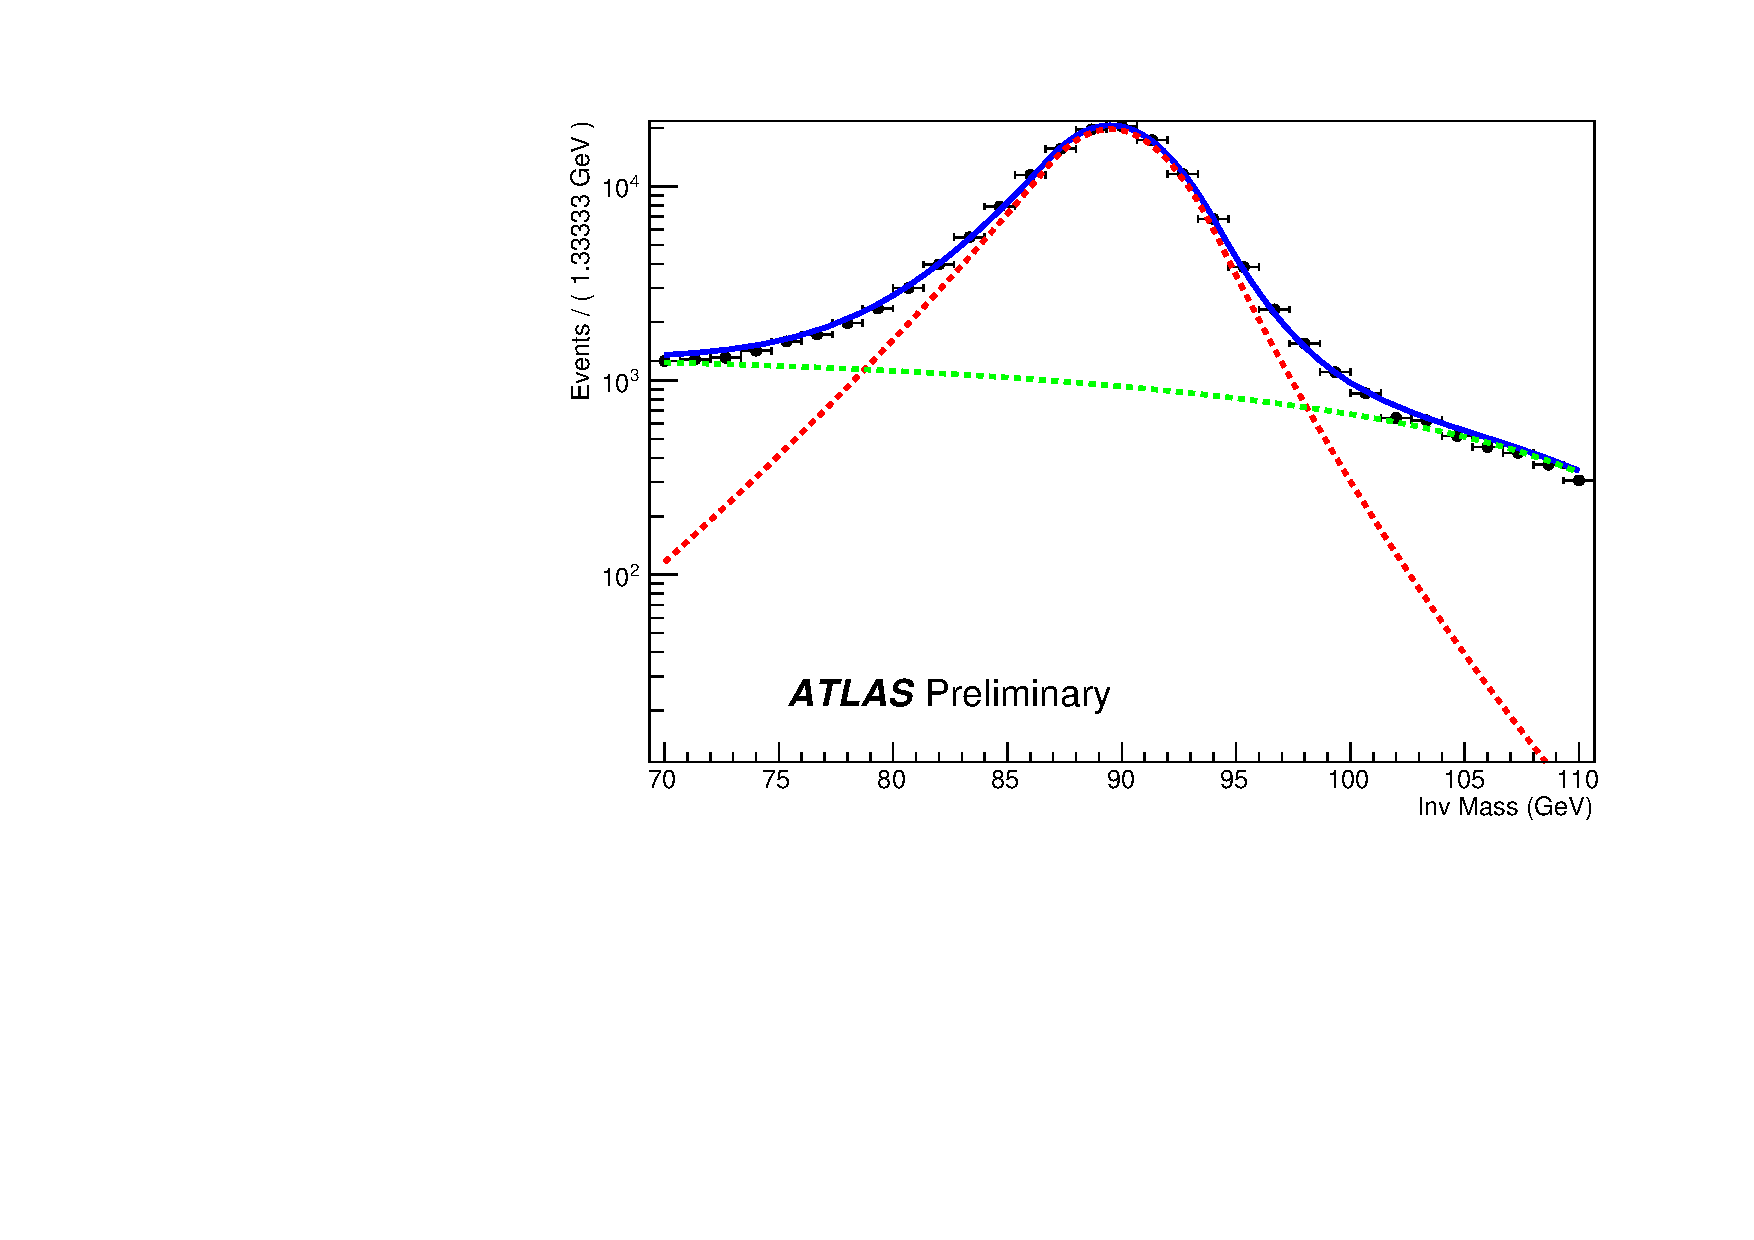
\includegraphics[scale=0.40]{d15_16_egam1_t_lmet_fit_h_m_eg_EE.pdf}
		\caption{Región EE}
	\end{subfigure}

	\caption{Ajuste de la masa invariante de los pares $ee$ (izquierda) y $e\gamma$ (derecha), para cada región de reconstrucción y para electrones \textit{tight}. La curva roja corresponde a la DSCB, la verde al polinomio de grado 2 y la azul a la combinación resultante de ambas.}
\label{fits_invmass_tight}
\end{figure}




\section{Resultados y estimación del fondo en regiones validación} \label{sec:resultados}


Los resultados obtenidos para el factor en bines de $\eta$ y $p_{T}$ para electrones \textit{medium} y \textit{tight} se muestran en la Tablas \ref{ta:fftable_medium} y \ref{ta:fftable_tight}, incluyendo por separada las incertezas estadísticas y sistemáticas del método. Se puede apreciar que este factor crece con $|\eta|$, dado que está relacionado con el incremento en el material del detector atravesado por los electrones y el incremento en la tasa de reconstrucción de fotones convertidos con una sola traza \cite{Alonso:2147473}.


\begin{table}	
\centering
\caption{Tabla con los factores de identificación errónea en bines de $\eta$ y $p_{T}$, con sus valores de incerteza estadística y sistemática, para electrones \textit{medium}.}
\begin{threeparttable}
\begin{tabular}{ l l c c c c c }

	\hline
	\hline

	\multirow{2}{*}{$|\eta|$} & \multirow{2}{*}{$p_{T}$[GeV]} & \multirow{2}{*}{Fake factor} & \multirow{2}{*}{Estadístico} & \multicolumn{3}{c}{Sistemáticos}  \\

	\cline{5-7}

	 		& & & 	& $w=1$ & Rango & Total \\


	\hline

	0 - 0.6 	& 75 - 90 	& 0.0149 & 0.0003 & 0.004	&  0.0004	&  0.004  \\

	0 - 0.6 	& 90 - 145 	& 0.0136 & 0.0004 & 0.004	&  0.0004	&  0.004  \\

	0 - 0.6 	& 145 - 300 & 0.0113 & 0.0008 & 0.003	&  0.0003	&  0.003  \\

	\hline

	0.6 - 1.37 	& 75 - 90 	& 0.0164 & 0.0003 & 0.004	&  0.0004	&  0.004  \\

	0.6 - 1.37 	& 90 - 145 	& 0.0157 & 0.0004 & 0.004	&  0.0003	&  0.004  \\

	0.6 - 1.37 	& 145 - 300 & 0.0116 & 0.0007 & 0.003	&  0.0003	&  0.003  \\

	\hline

	1.52 - 1.82 & 75 - 90 	& 0.034  & 0.001 & 0.005	&  0.0005	&  0.005 \\

	1.52 - 1.82 & 90 - 145 	& 0.030  & 0.001 & 0.005	&  0.001	&  0.005  \\

	1.52 - 1.82 & 145 - 300 & 0.023  & 0.002 & 0.003	&  0.0005	&  0.003  \\

	\hline

	1.82 - 2.37 & 75 - 90 	& 0.044		& 0.001 & 0.006	&  0.002	&  0.006  \\

	1.82 - 2.37 & 90 - 145	& 0.038		& 0.001 & 0.005	&  0.001	&  0.005  \\

	1.82 - 2.37 & 145 - 300 & 0.039		& 0.003 & 0.006	&  0.001	&  0.006  \\

	\hline
	\hline

\end{tabular}
\end{threeparttable}
\label{ta:fftable_medium}
\end{table}

\begin{table}	
\centering
\caption{Tabla con los factores de identificación errónea en bines de $\eta$ y $p_{T}$, con sus valores de incerteza estadística y sistemática, para electrones \textit{tight}.}
\begin{threeparttable}
\begin{tabular}{ l l c c c c c }

	\hline
	\hline

	\multirow{2}{*}{$|\eta|$} & \multirow{2}{*}{$p_{T}$[GeV]} & \multirow{2}{*}{Fake factor} & \multirow{2}{*}{Estadístico} & \multicolumn{3}{c}{Sistemáticos} \\
	
	\cline{5-7}

	 & & & & $w=1$ & Rango & Total \\

	\hline

	0 - 0.6 	& 75 - 90 	& 0.0155 & 0.0004 & 0.004	&  0.001	&  0.004  \\

	0 - 0.6 	& 90 - 145 	& 0.0141 & 0.0004 & 0.004	&  0.002	&  0.004  \\

	0 - 0.6 	& 145 - 300 & 0.0116 & 0.0008 & 0.002	&  0.001	&  0.003  \\

	\hline

	0.6 - 1.37 	& 75 - 90 	& 0.0173 & 0.0004 & 0.004	&  0.002	&  0.004  \\

	0.6 - 1.37 	& 90 - 145 	& 0.0161 & 0.0004 & 0.004	&  0.002	&  0.004  \\

	0.6 - 1.37 	& 145 - 300 & 0.0121 & 0.0008 & 0.003	&  0.002	&  0.003  \\

	\hline

	1.52 - 1.82 & 75 - 90 	& 0.036  & 0.001 & 0.005	&  0.002	&  0.005 \\

	1.52 - 1.82 & 90 - 145 	& 0.033  & 0.001 & 0.004	&  0.003	&  0.005  \\

	1.52 - 1.82 & 145 - 300 & 0.022  & 0.002 & 0.003	&  0.001	&  0.003  \\

	\hline

	1.82 - 2.37 & 75 - 90 	& 0.046		& 0.001 & 0.007	&  0.002	&  0.007  \\

	1.82 - 2.37 & 90 - 145	& 0.039		& 0.001 & 0.006	&  0.003	&  0.007  \\

	1.82 - 2.37 & 145 - 300 & 0.041		& 0.003 & 0.006	&  0.002	&  0.006  \\

	\hline
	\hline

\end{tabular}
\end{threeparttable}
\label{ta:fftable_tight}
\end{table}

% \begin{table}	
% \centering
% \begin{threeparttable}
% \caption{Tabla con los factores de identificación errónea en bines de $\eta$ y $p_{T}$, con sus valores de incerteza estadística y sistemática.}
% \begin{tabular}{ l l c c c }

% 	\hline
% 	\hline

% 	$|\eta|$ & $p_{T}$[GeV] & Fake factor & Estadísticos & Sistemáticos \\

% 	\hline

% 	0 - 0.6 & 75 - 90 & 0.0168 & 0.0003 & -		 \\

% 	0 - 0.6 & 90 - 145 & 0.0158 & 0.0004 & - 	 \\

% 	0 - 0.6 & 145 - 300 & 0.0142 & 0.0007 & -  	 \\

% 	\hline

% 	0.6 - 1.37 & 75 - 90 & 0.0186 & 0.0003 & -	 \\

% 	0.6 - 1.37 & 90 - 145 & 0.0183 & 0.0004 & -	 \\

% 	0.6 - 1.37 & 145 - 300 & 0.0141 & 0.0007 & -   \\

% 	\hline

% 	1.52 - 1.82 & 75 - 90 & 0.0354  & 0.0009 &  \\

% 	1.52 - 1.82 & 90 - 145 & 0.033  & 0.001 & \\

% 	1.52 - 1.82 & 145 - 300 & 0.026  & 0.002 & \\

% 	\hline

% 	1.82 - 2.37 & 75 - 90 & 0.045  & 0.001 &  \\

% 	1.82 - 2.37 & 90 - 145 & 0.040  & 0.001 &  \\

% 	1.82 - 2.37 & 145 - 300 & 0.038  & 0.002 & \\

% 	\hline
% 	\hline

% \end{tabular}
% \label{ta:fftable}
% \end{threeparttable}
% \end{table}

Observando los resultados expuestos en las distintas tablas, definimos la implementación de una selección \textit{medium} de los electrones ya que los valores de pureza (expresado en los valores de los pesos $w$) e incertezas sistemáticas son equivalentes a la selección \textit{tight}, pero con la ventaja de una probable mayor estadística de eventos para estimar el fondo en las distintas regiones de control y validación.


Con el objetivo de validar los resultados obtenidos, se realizo una búsqueda de una nueva región de validación donde el fondo predominante sea el de eventos con electrones erróneamente reconstruidos. Los criterios para determinar la VR se pueden observar en la Tabla \ref{ta:vr_crit}. Estos criterios seleccionan de forma predominante eventos $W(e\nu)$ + jets, donde un $W$ con alta energía cinética, decae en un neutrino (asociado con una alta $\met$) y electrón de alto $p_{T}$ (identificado como fotón), son colineales entre sí ($\Delta\phi<0.4$). La contribución de cada fondo al número de eventos en esta región se puede observar en la Tabla \ref{ta:vr_events}, en donde se puede observar que para esta región el fondo proveniente de electrones mal reconstruidos como fotones es el que predomina ($\sim63\%$) y se observa comparativamente un excelente acuerdo entre los datos esperados y obtenidos. Las distribuciones para $\Delta \phi$ y $\met$ se observan en la Figura \ref{VRE_dphi_met}, donde se observa un excelente acuerdo entre las los resultados esperados y los datos obtenidos.

Los resultados mostrados permiten entonces validar el método y sus predicciones, y poder ser así utilizados para predecir la cantidad de eventos esperados en las distintas regiones de señal.

\begin{table}
\centering
\caption{Criterios de selección para la región de validación \cite{drfran}.}
  \begin{tabular}{l|r}
  \hline
  \hline
  & VRE \\
  \hline
  $N_{\mathrm{fotones}}$                  &       $\ge1$  \\
  $\pt^{\text{leading}\: \gamma} >$         &    $145\egev$  \\
  $N_{\mathrm{leptones}}$                  &           -   \\
  $N_{\mathrm{jets}}$                     &       $\ge1$  \\
  $N_{b-\mathrm{jets}}$                   &       $\ge1$  \\
  $\Delta\phi(\text{jet}, \met)$          &       $>0.4$  \\
  $\Delta\phi(\gamma, \met)$                &       $<0.4$  \\
  ${\met}$                                &   $>200\egev$  \\
  $m_{\text{eff}}$                               &  $[500, 2000]\egev$  \\
  \hline
  \hline
\end{tabular}
\label{ta:vr_crit}
\end{table}

\begin{table}
\centering
\caption{Contribución de cada fondo a la región de validación. Las incertezas mostradas son solo sistemáticas \cite{drfran}.}
\begin{tabular}{lr}
\hline
 & $e\to\gamma$ falsos VR \\
\hline
Eventos observados & 94 \\
\hline
Eventos esperados por el SM & $92.18 \pm 12.58$ \\
\hline
$\gamma$ + jets & $1.46 \pm 0.16$ \\
$W\gamma$ & $13.73 \pm 1.26$ \\
$Z\gamma$ & $0.87 \pm 0.05$ \\
$\ttbar\gamma$ & $4.91 \pm 0.70$ \\
$e\rightarrow\gamma$ falsos & $58.43 \pm 12.49$ \\
$\text{jets}\rightarrow\gamma$ falsos & $12.73 \pm 2.14$ \\
$\gamma\gamma / W\gamma\gamma / Z\gamma\gamma$ & $0.05 \pm 0.00$ \\
\hline
\end{tabular}
\label{ta:vr_events}
\end{table}


\begin{figure}
\centering
	\begin{subfigure}{0.45\textwidth}
		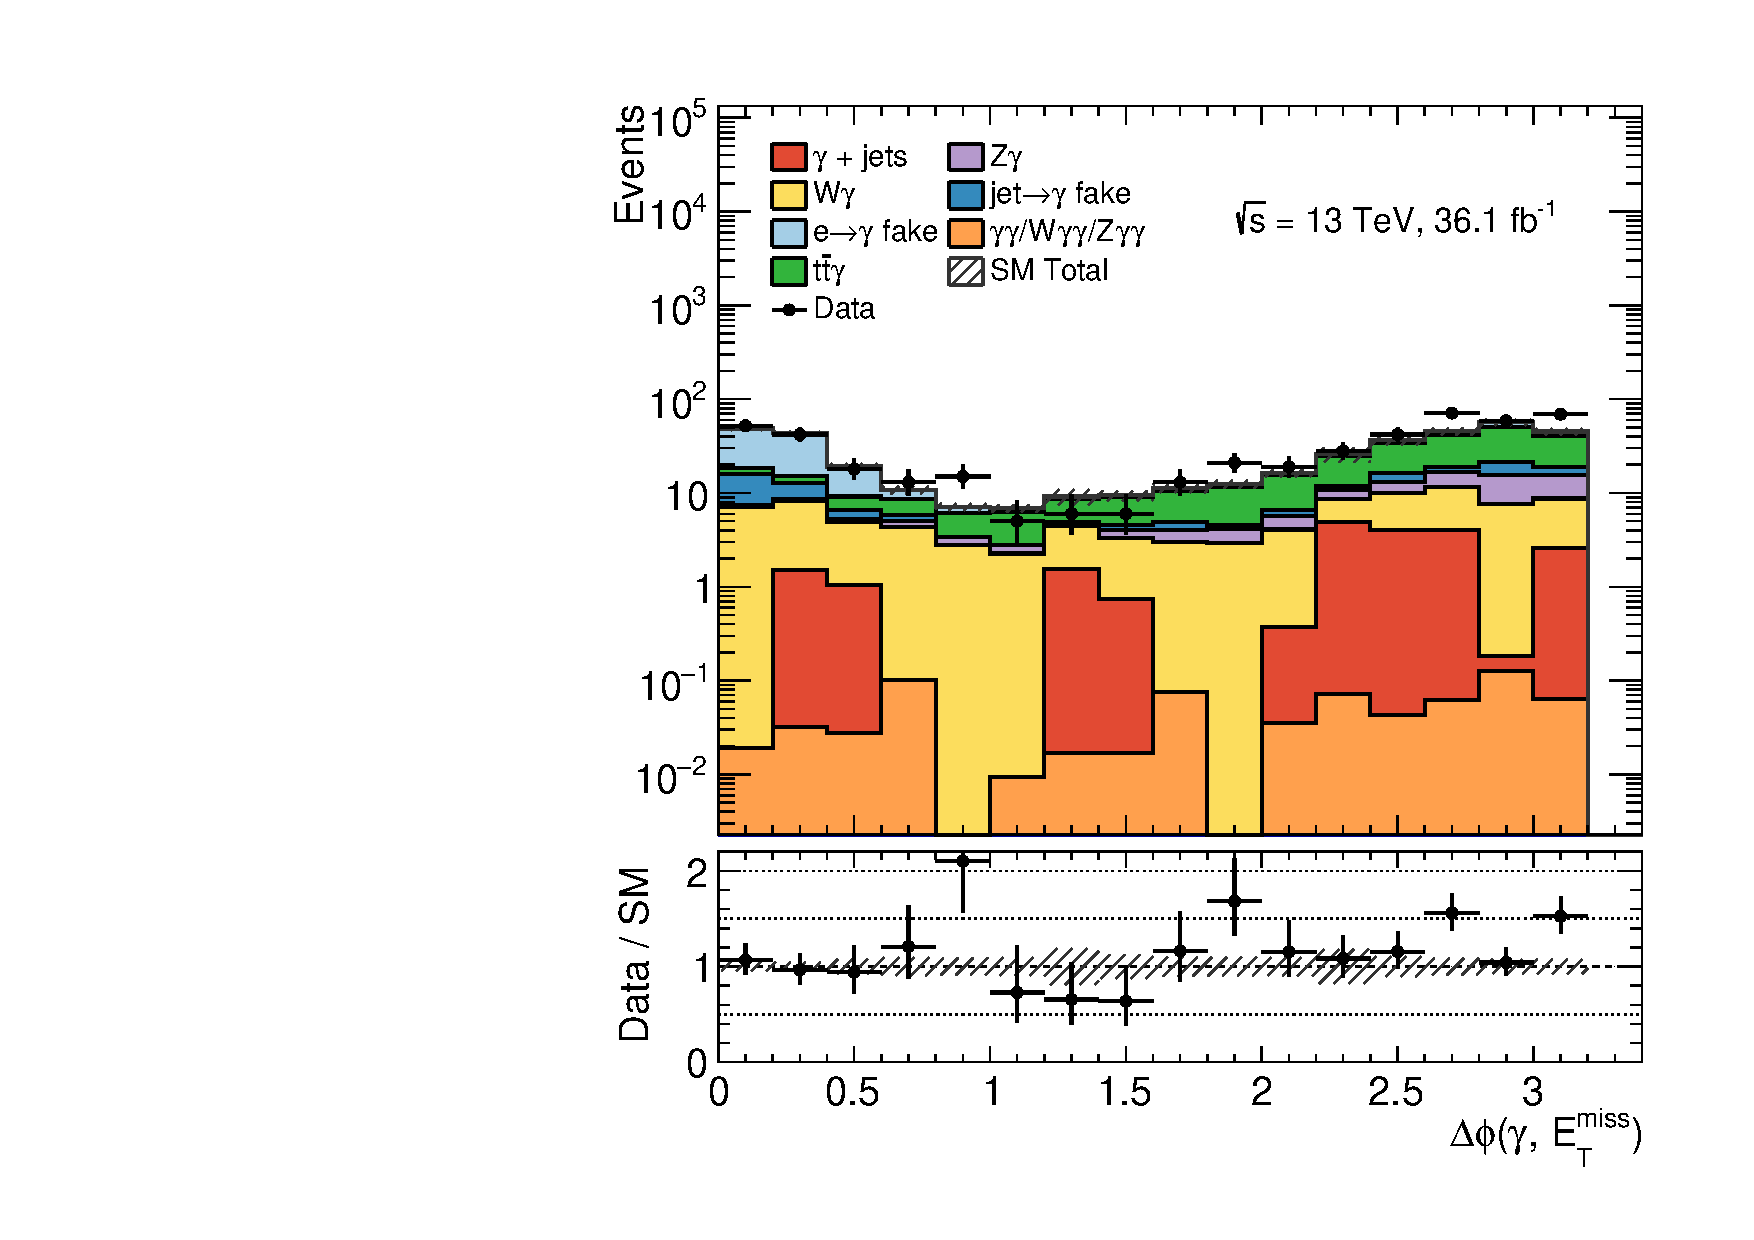
\includegraphics[scale=0.35]{can_VRE_dphi_gammet_afterFit.pdf}
	\end{subfigure}
	~
	\begin{subfigure}{0.45\textwidth}
		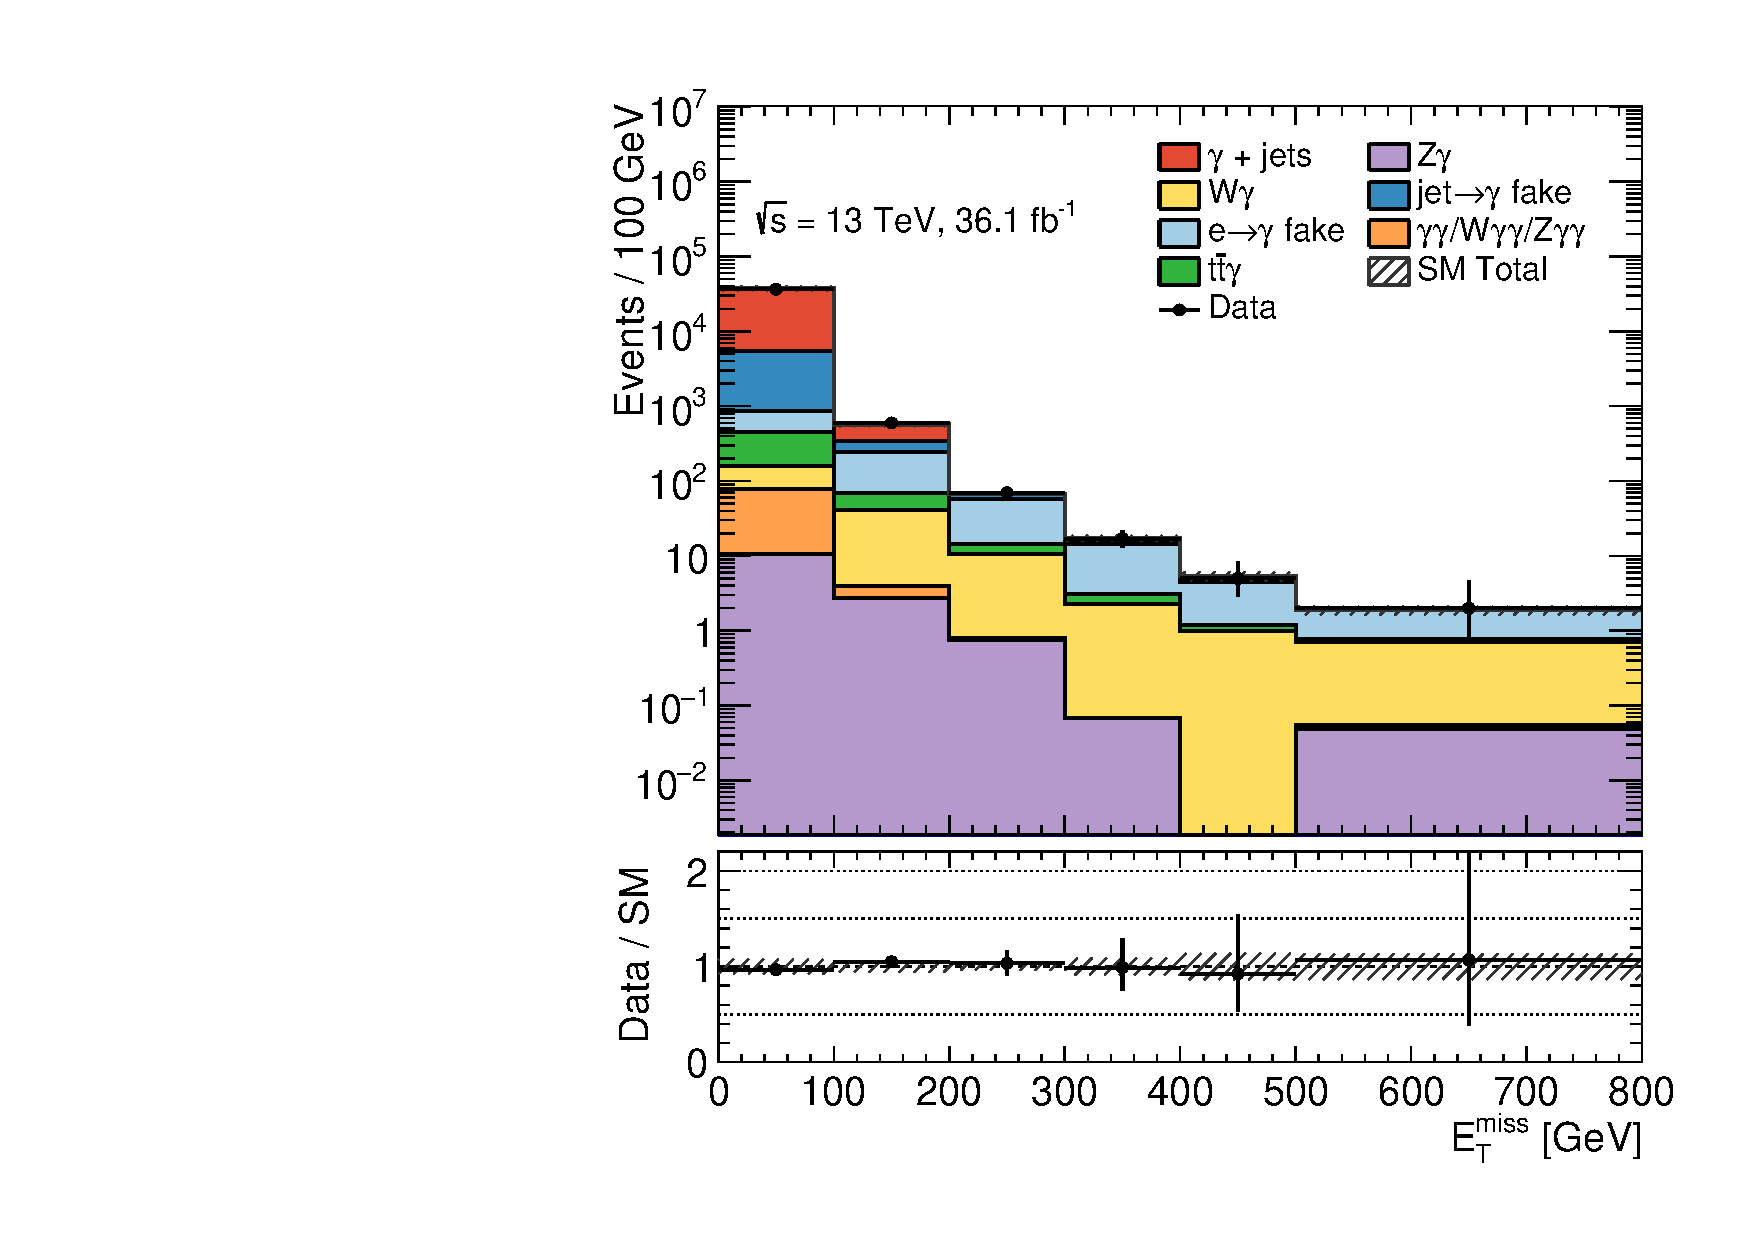
\includegraphics[scale=0.35]{can_VRE_met_et_afterFit.pdf}
	\end{subfigure}
\caption{Distribución de $\Delta \phi$ (izquierda) y  $\met$ (derecha) para una región de validación. La variable mostrada se deja libre en el gráfico, mientras el resto de la variables se mantienen con los cortes propuestos en la VRE. Las incertezas mostradas son solo estadísticas \cite{drfran}.}
\label{VRE_dphi_met}
\end{figure}




\clearpage

\chapter{Conclusiones}
% \addcontentsline{toc}{chapter}{Conclusión}
\chaptermark{Conclusiones}

Supersimetría se ha vuelto uno de los principales objetivos del LHC en los últimos años para la búsqueda de nueva física. Esa búsqueda consiste en encontrar eventos por encima de los ya predichos por el SM, que toman el rol de fondo en la búsqueda de SUSY. El hallazgo de un exceso en los datos sobre las predicciones del SM abrirán el camino para dar respuesta a los interrogantes actuales en física de partículas. En el caso de que los datos sean compatibles con las predicciones del SM se pondrán nuevas cotas en los parámetros de teorías de nueva física, en particular de nuevas partículas predichas por SUSY. En ambos casos los resultados nos permitirán avanzar en nuestra comprensión de la naturaleza. 

En esta tesis se ha presentado un estudio de la producción de eventos de $W$/$Z$ + jets o $\ttbar$ , en procesos donde un electrón del estado final es reconstruido como un fotón, contaminando así la búsqueda de nuevas partículas en regiones de señal que contienen fotones, jets y energía faltante en el estado final. En particular, se implementó un método para poder estimar este tipo de procesos utilizando información de los datos colectados por el detector ATLAS durante el Run 2 del LCH en los años 2015 y 2016.

Los resultados obtenidos en esta tesis son compatibles con predicciones en base a datos del 2015 y técnicas anteriores anteriores \cite{Alonso:2147473} \cite{Schumm:1994343} \cite{Collaboration:2198651} y fueron validados en el marco de esta Tesis, en las denominadas regiones de control y validación. Se concluye además, una independencia del método en los criterios de identificación de los electrones, pudiendo ser estos tanto \textit{medium} como \textit{tight}.

Al presente, los resultados mostrados en este trabajo están siendo implementados por la colaboración ATLAS para estimar el conjunto total de fondos del SM en las regiones de señal en la búsqueda partículas superimétricas con decaimiento y presencia de fotones en el estado final.



% \vfill

%%
%%   Bibliography
%%   ============

% \bibliographystyle{unsrt}
\bibliographystyle{bibtex/bst/atlasBibStyleWoTitle}
\bibliography{bibtex/bib/reference.bib,bibtex/bib/ATLAS.bib,bibtex/bib/ConfNotes.bib,bibtex/bib/PubNotes.bib,bibtex/bib/Extra.bib}
%\addbibresource{reference.bib}
%\addbibresource{bibtex/bib/ATLAS.bib}
%\addbibresource{bibtex/bib/ConfNotes.bib}
%\addbibresource{bibtex/bib/PubNotes.bib}

\addcontentsline{toc}{chapter}{Bibliografia}  

%%
%%   Appendix
%%   ============

% \begin{appendix}
% \input{/user/wahlberg/Thesis/conventions}
% \end{appendix}

% \input{/user/wahlberg/Thesis/summary.tex}
% \input{/user/wahlberg/Thesis/samenvatting.tex}
% \input{/user/wahlberg/Thesis/ack.tex}

%\thispagestyle{empty}

\end{document}











